%Comment Legend
%TODO marks a todo item

% Before publishing / submitting:
%TODO spell check

\documentclass[sort&compress]{elsarticle}
\usepackage[utf8]{inputenc}
\usepackage{natbib}
\usepackage{graphicx}
\usepackage{amsmath}
\usepackage[parfill]{parskip}
\usepackage{hyperref}

% https://www.tug.org/pipermail/tex-live/2012-August/032161.html
\makeatletter
\providecommand{\doi}[1]{
  \begingroup
    \let\bibinfo\@secondoftwo
    \urlstyle{rm}
    \href{http://dx.doi.org/#1}{
      doi:\discretionary{}{}{}
      \nolinkurl{#1}
    }
  \endgroup
}
\makeatother

\usepackage[nameinlink,noabbrev]{cleveref}
\usepackage{amssymb}
\usepackage[printonlyused, withpage, nolist,nohyperlinks]{acronym}
\usepackage[]{algorithm2e}
\usepackage{booktabs} % used by pandas to_latex
\usepackage{newunicodechar} % using ∞ in pandas
\newunicodechar{∞}{$\infty$}
\newunicodechar{α}{$\alpha$}
\usepackage[table]{xcolor}
% slanted table headings
% https://tex.stackexchange.com/a/32690/33609
\usepackage{adjustbox}
\usepackage{array}
\newcolumntype{R}[2]{%
    >{\adjustbox{angle=#1,lap=\width-(#2)}\bgroup}%
    l%
    <{\egroup}%
}
\newcommand*\rot{\multicolumn{1}{R{60}{1em}}}% no optional argument here, please!
\usepackage{makecell}
\usepackage{caption}
\usepackage[margin=1in]{geometry}

\newlength\kwInLength
\newcommand\kwInMultiline[1]{%
  \settowidth\kwInLength{\KwIn{}}%
  \setlength\hangindent{\kwInLength}%
  \hspace*{\kwInLength}#1\\}

\newcommand{\vect}[1]{\boldsymbol{#1}}

\mathchardef\mhyphen="2D

\graphicspath{ {images/} }

\begin{acronym}[TT]
	\acro{A-SUWO}{adaptive semi-unsupervised weighted oversampling}
	\acro{AUPRC}{area under the precision-recall curve}
	\acro{GBM}{gradient boosting machine}
	\acro{KNN}{k-nearest neighbors}	
	\acro{LR}{logistic regression}
	\acro{PR}{precision-recall}
	\acro{SMOTE}{synthetic minority over-sampling technique}
	\acro{SOMO}{self-organizing map oversampling}

	\acrodefplural{LR}[LR]{Logistic regression}
	\acrodefplural{PR}[PR]{Precision-recall}
\end{acronym}

\begin{document}

\begin{frontmatter}

\title{Improving Imbalanced Learning \\Through a Heuristic Oversampling Method \\Based on K-Means and SMOTE}

\author[nova]{Georgios Douzas}
\ead{gdouzas@icloud.com}
\author[nova]{Fernando Bacao\corref{correspondingauthor}}
\ead{bacao@novaims.unl.pt}
\author[nova]{Felix Last}
\ead{mail@felixlast.de}
\cortext[correspondingauthor]{Corresponding author}
\address[nova]{Nova Information Management School, Campus de Campolide, 1070-312 Lisboa, Portugal \\ Telephone: +351 21 382 8610}

\begin{abstract}
Learning from class-imbalanced data continues to be a common and challenging
problem in supervised learning as standard classification algorithms are
designed to handle balanced class distributions. While different strategies
exist to tackle this problem, methods which generate artificial data to achieve
a balanced class distribution are more versatile than modifications to the
classification algorithm. Such techniques, called oversamplers, modify the
training data, allowing any classifier to be used with class-imbalanced
datasets. Many algorithms have been proposed for this task, but most are complex
and tend to generate unnecessary noise. This work presents a simple and
effective oversampling method based on k-means clustering and SMOTE (synthetic
minority oversampling technique), which avoids the generation of noise and
effectively overcomes imbalances between and within classes. Empirical results
of extensive experiments with 90 datasets show that training data oversampled
with the proposed method improves classification results. Moreover, k-means
SMOTE consistently outperforms other popular oversampling methods. An
implementation\footnote{The implementation of k-means \acs{SMOTE} can be found
at \url{https://github.com/felix-last/kmeans_smote}.} is made available in the
Python programming language.
\end{abstract}

\begin{keyword}
Class-Imbalanced Learning\sep Oversampling\sep Classification\sep Clustering\sep Supervised Learning\sep Within-Class Imbalance
\end{keyword}

\end{frontmatter}

\pagenumbering{arabic} % NOVA

\section{Introduction}
% \subsection{The Class Imbalance Problem}
The class imbalance problem in machine learning describes classification tasks
in which classes of data are not equally represented. In many real-world
applications, the nature of the problem implies a sometimes heavy skew in the
class distribution of a binary or multi-class classification problem. Such
applications include fraud detection in banking, rare medical diagnoses, and oil
spill recognition in satellite images, all of which naturally exhibit a minority
class~\citep{Chawla.2002,Kotsiantis.2006,Kotsiantis.2007,Galar.2012}.

The predictive capability of classification algorithms is impaired by class
imbalance. Many such algorithms aim at maximizing classification accuracy, a
measure which is biased towards the majority class. A classifier can achieve
high classification accuracy even when it does not predict a single minority
class instance correctly. For example, a trivial classifier which scores all
credit card transactions as legit will score a classification accuracy of 99.9\%
assuming that 0.1\% of transactions are fraudulent; however in this case, all
fraud cases remain undetected. In conclusion, by optimizing classification
accuracy, most algorithms assume a balanced class
distribution~\citep{Provost.2000,Kotsiantis.2007}.

Another inherent assumption of many classification algorithms is the uniformity
of misclassification costs, which is rarely a characteristic of real-world
problems. Typically in imbalanced datasets, misclassifying the minority class as
the majority class has a higher cost associated with it than vice versa. An
example of this is database marketing, where the cost of mailing to a
non-respondent is much lower than the lost profit of not mailing to a
respondent~\citep{Domingos.1999}.

Lastly, what is referred to as the ``small disjuncts problem'' is often
encountered in imbalanced datasets~\citep{Galar.2012}. The problem refers to
classification rules covering only a small number of training examples. The
presence of only few samples make rule induction more susceptible to
error~\citep{Holte.1989}. To illustrate the importance of discovering high
quality rules for sparse areas of the input space, the example of credit card
fraud detection is again considered. Assume that most fraudulent transactions
are processed outside the card owner's home country. The remaining cases of
fraud happen within the country, but show some different exceptional
characteristic, such as a high amount, an unusual time or recurring charges.
Each of these other characteristics applies to only a very small group of
transactions, which by itself is often vanishingly small. However, adding up all
these edge cases, they can make up a substantial portion of all fraudulent
transactions. Therefore, it is important that classifiers pay adequate attention
to small disjuncts~\citep{Holte.1989}.

Techniques aimed at improving classification in the presence of class imbalance
can be divided into three broad categories\footnote{The three categories are not
exhaustive and new categories have been introduced, such as the combination of
each of these techniques with ensemble
learning~\citep{Galar.2012,Diez-pastor.2015,Galar.2016}.}: algorithm level
methods, data level methods, and cost-sensitive methods.

Solutions which modify the classification algorithm to cope with the imbalance
are algorithm level techniques~\citep{Kotsiantis.2006,Galar.2012}. Such
techniques include changing the decision threshold and training separate
classifiers for each class~\citep{Kotsiantis.2006,Chawla.2004}. 

In contrast, cost-sensitive methods aim at providing classification algorithms
with different misclassification costs for each class. This requires knowledge
of misclassification costs, which are dataset-dependent and commonly unknown or
difficult to quantify. Additionally, the algorithms must be capable of
incorporating the misclassification cost of each class or instance into their
optimization. Therefore, these methods are regarded as operating both on data
and algorithm level~\citep{Galar.2012}.

Finally, data-level methods manipulate the training data, aiming to change the
class distribution towards a more balanced one. Techniques in this category
resample the data by removing cases of the majority classes (undersampling) or
adding instances to the minority classes by means of duplication or generation
of new samples (oversampling)~\citep{Kotsiantis.2006,Galar.2012}. Because
undersampling removes data, such methods risk the loss of important concepts.
Moreover, when the number of minority observations is small, undersampling to a
balanced distribution yields an undersized dataset, which may in turn limit
classifier performance. Oversampling, on the other hand, may encourage
overfitting when observations are merely duplicated~\citep{Weiss.2007}. This
problem can be avoided by adding genuinely new samples. One straightforward
approach to this is \ac{SMOTE}, which interpolates existing samples to generate
new instances. 

Data-level methods can be further discriminated into random and informed
methods. Unlike random methods, which randomly choose samples to be removed or
duplicated, informed methods take into account the distribution of the
samples~\citep{Chawla.2004}. This allows informed methods to direct their
efforts to critical areas of the input space, for instance to sparse
areas~\citep{Nickerson.2001}, safe areas~\citep{Bunkhumpornpat.2009}, or to
areas close to the decision boundary~\citep{Han.2005}. Consequently, informed
methods may avoid the generation of noise and can tackle imbalances within
classes.

Unlike algorithm-level methods, which are bound to a specific classifier, and
cost-sensitive methods, which are problem-specific and need to be implemented by
the classifier, data-level methods can be universally applied and are therefore
more versatile~\citep{Galar.2012}.

Many oversampling techniques have proven to be effective in real-world domains.
\ac{SMOTE} is the most popular oversampling method that was proposed to improve
random oversampling. There are multiple variations of \ac{SMOTE} which aim to
combat the original algorithm's weaknesses. Yet, many of these approaches are
either very complex or alleviate only a few of \ac{SMOTE}'s shortcomings.
Additionally, few of them are readily available in a unified software framework
used by practitioners.

This paper suggests the combination of the k-means clustering algorithm with
\ac{SMOTE} to combat some of other oversampler's shortcomings with a
simple-to-use technique. The use of clustering enables the proposed oversampler
to identify and target areas of the input space where the generation of
artificial data is most effective. The method aims at eliminating both
between-class imbalances and within-class imbalances while at the same time
avoiding the generation of noisy samples. Its appeal is the widespread
availability of both underlying algorithms as well the effectiveness of the
method itself.

While the proposed method could be extended to cope with multi-class problems,
the focus of this work is placed on binary classification tasks. When working
with more than two imbalanced classes, different aspects of classification, as
well as evaluation, must be considered, which is discussed in detail by
\citet{Fernandez.2013}.

The remainder of this work is organized as follows. In \cref{sec:related-work},
related work is summarized and currently available oversampling methods are
introduced. Special attention is paid to oversamplers which - like the proposed
method - employ a clustering procedure. \Cref{sec:proposed-method} explains in
detail how the proposed oversampling technique works and which hyperparameters
need to be tuned. It is shown that both \ac{SMOTE} and random oversampling are
limit cases of the algorithm and how they can be achieved. In
\cref{sec:research-methodology}, a framework aimed at evaluating the performance
of the proposed method in comparison with other oversampling techniques is
established. The experimental results are shown in
\cref{sec:experimental-results}, which is followed by \cref{sec:conclusion}
presenting the conclusions.

\section{Related Work}
\label{sec:related-work}

Methods to cope with class imbalance either alter the classification algorithm
itself, incorporate misclassification costs of the different classes into the
classification process, or modify the data used to train the classifier.
Resampling the training data can be done by removing majority class samples
(undersampling) or by inflating the minority class (oversampling). Oversampling
techniques either duplicate existing observations or generate artificial data.
Such methods may work uninformed, randomly choosing samples which are replicated
or used as a basis for data generation, or informed, directing their efforts to
areas where oversampling is deemed most effective. Among informed oversamplers,
clustering procedures are sometimes applied to determine suitable areas for the
generation of synthetic samples.

Random oversampling randomly duplicates minority class instances until the
desired class distribution is reached. Due to its simplicity and ease of
implementation, it is likely to be the method that is most frequently used among
practitioners. However, since samples are merely replicated, classifiers trained
on randomly oversampled data are likely to suffer from
overfitting\footnote{Overfitting occurs when a model does not conform with the
principle of parsimony. A flexible model with more parameters than required is
predisposed to fit individual observations rather than the overall distribution,
typically impairing the model's ability to predict unseen
data~\citep{Hawkins.2004}. In random oversampling, overfitting may occur when
classifiers construct rules which seemingly cover multiple observations, while
in fact they only cover many replicas of the same
observation~\citep{Batista.2004}.}~\citep{Batista.2004,Chawla.2004}.

In 2002, \citet{Chawla.2002} suggested the \ac{SMOTE} algorithm, which avoids
the risk of overfitting faced by random oversampling. Instead of merely
replicating existing observations, the technique generates artificial samples.
As shown in  \cref{fig:smote-illustration}, this is achieved by linearly
interpolating a randomly selected minority observation and one of its
neighboring minority observations. More precisely, \ac{SMOTE} executes three
steps to generate a synthetic sample. Firstly, it chooses a random minority
observation $\vec{a}$. Among its $k$ nearest minority class neighbors, instance
$\vec{b}$ is selected. Finally, a new sample $\vec{x}$ is created by randomly
interpolating the two samples: $\vec{x} = \vec{a} + w \times (\vec{b} -
\vec{a})$, where $w$ is a random weight in $[0,1]$.

\begin{figure}[ht]
    \centering
	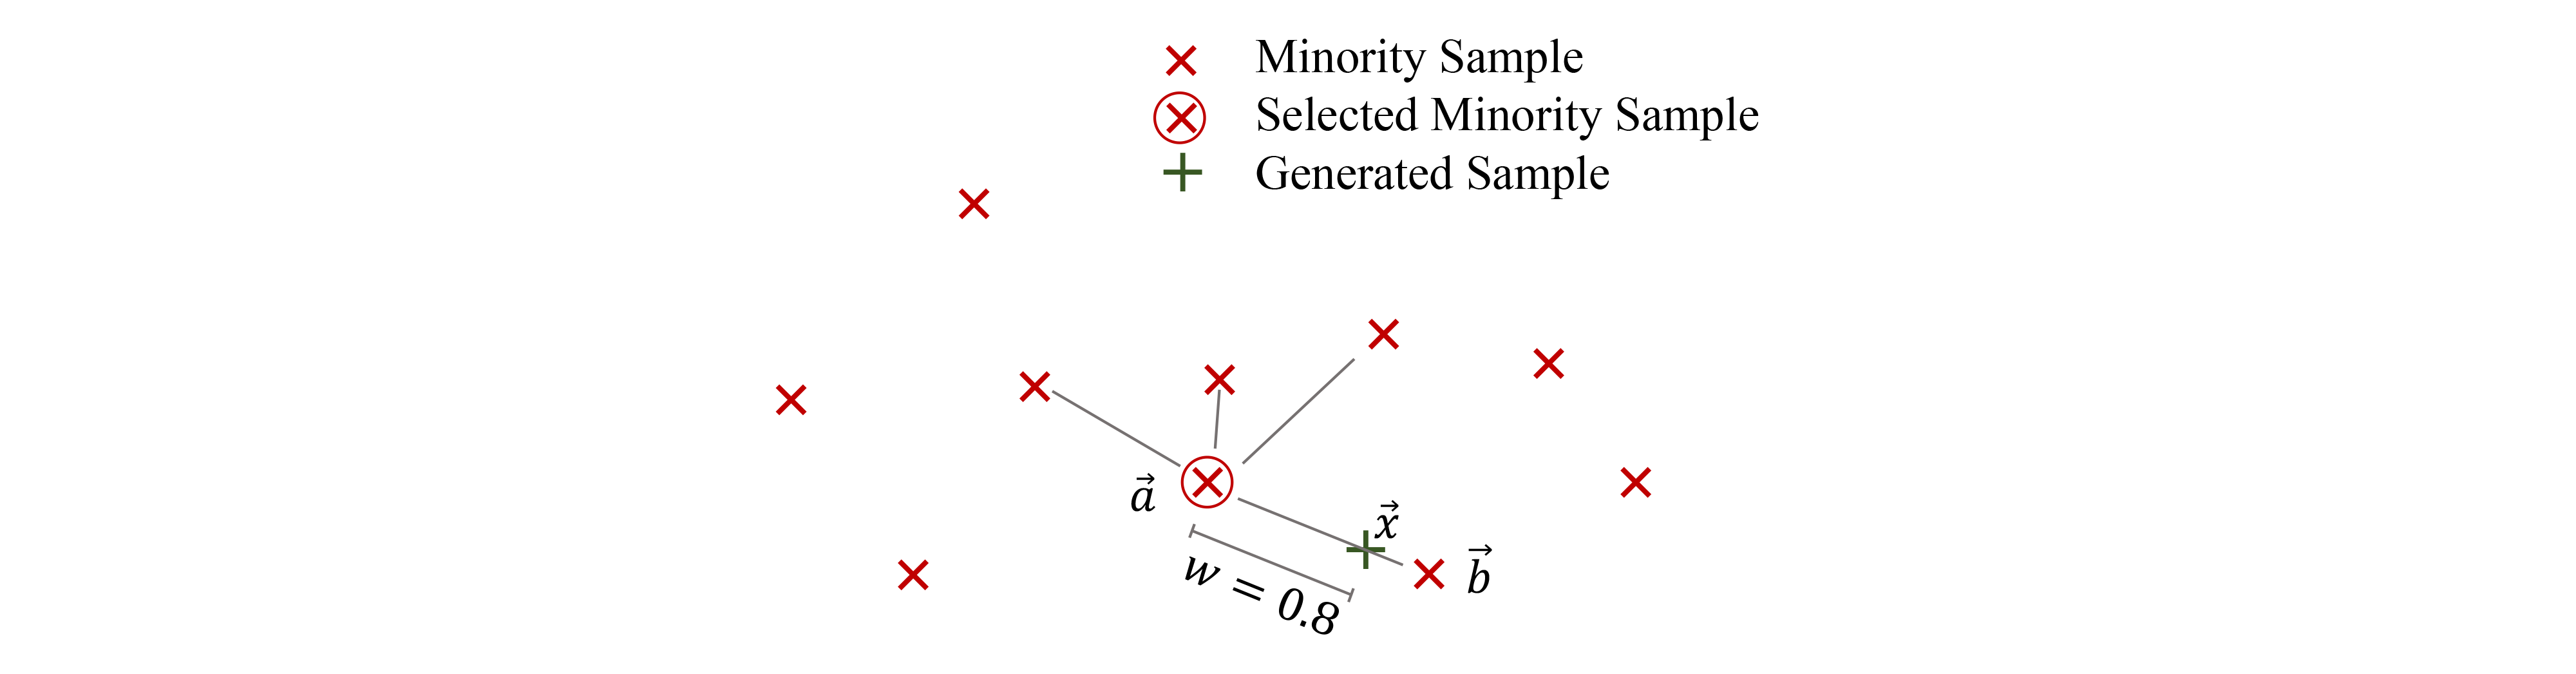
\includegraphics[width=1\textwidth]{../analysis/smote-illustration.png}
	\caption{\acs{SMOTE} linearly interpolates a randomly selected minority 
	sample and one of its $k=4$ nearest neighbors}
	\label{fig:smote-illustration}
\end{figure}

However, the algorithm has some weaknesses dealing with imbalance and noise as
illustrated in \cref{fig:smote-noisy-samples}. One such drawback stems from the
fact that \ac{SMOTE} randomly chooses a minority instance to oversample with
uniform probability. While this allows the method to effectively combat
between-class imbalance, the issues of within-class imbalance and small
disjuncts are ignored. Input areas counting many minority samples have a high
probability of being inflated further, while sparsely populated minority areas
are likely to remain sparse~\citep{Prati.2004}.

Another major concern is that \ac{SMOTE} may further amplify noise present in
the data. This is likely to happen when linearly interpolating a noisy minority
sample, which is located among majority class instances, and its nearest
minority neighbor. The method is susceptible to noise generation because it
doesn't distinguish overlapping class regions from so-called safe
areas~\citep{Bunkhumpornpat.2009,Rivera.2017,Zhu.2017,Saez.2015}. 

\begin{figure}[ht]
    \centering
	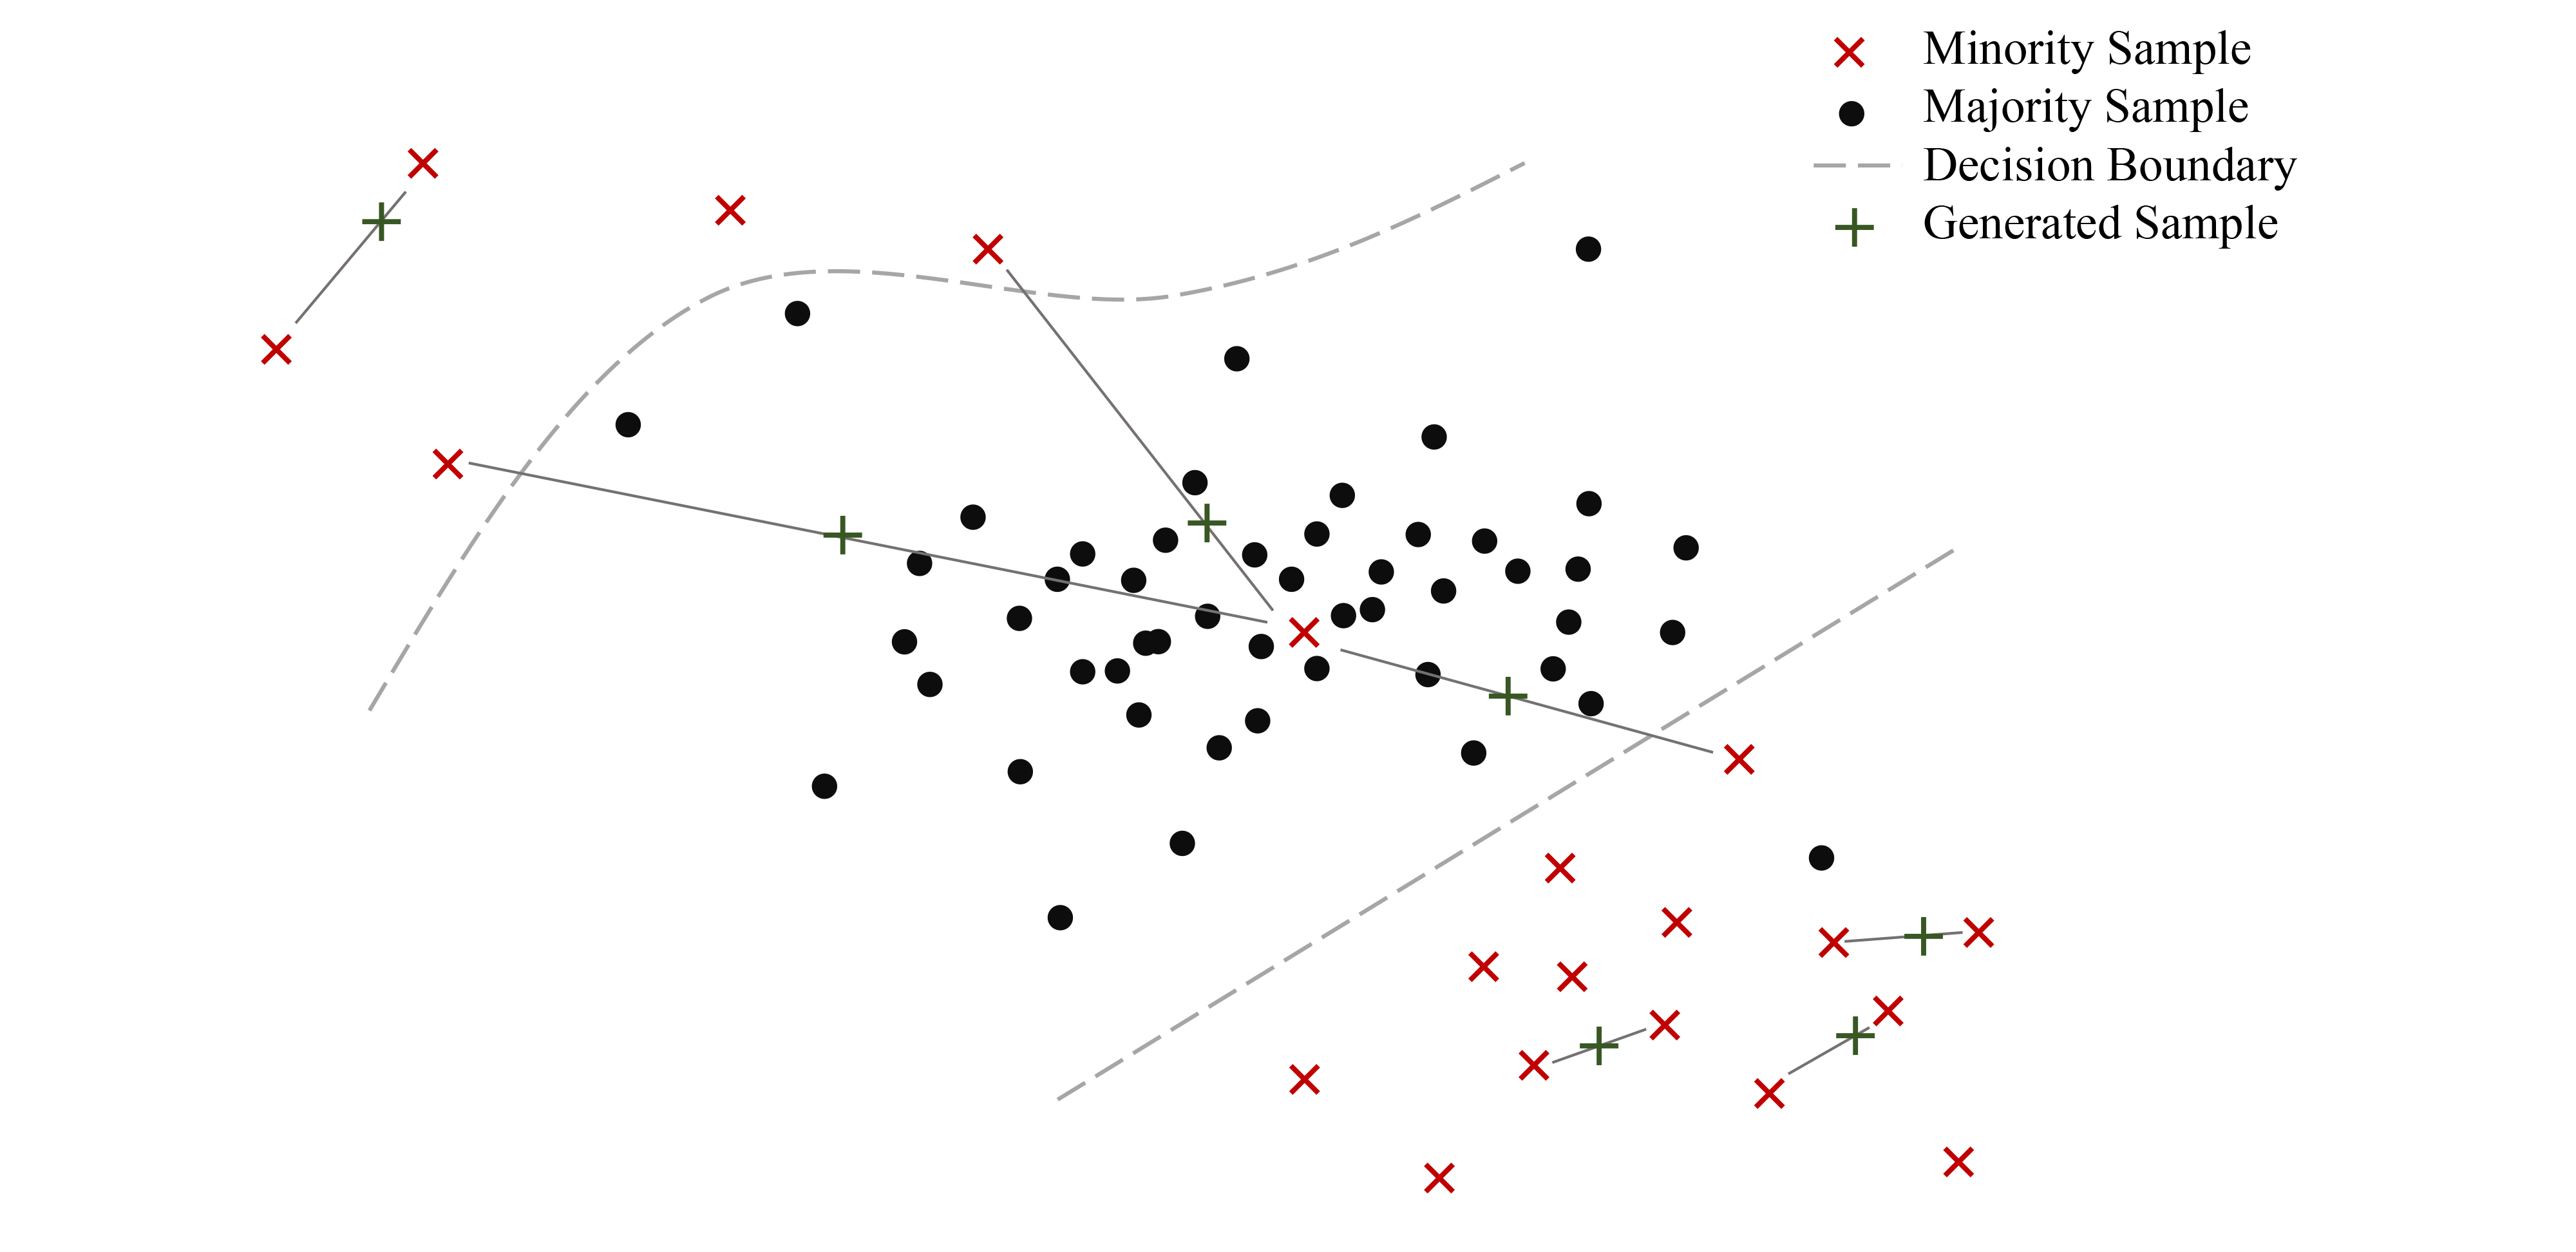
\includegraphics[width=1\textwidth]{../analysis/smote-noisy-samples.png}
	\caption[Behavior of \acs{SMOTE} in the presence of noise and within-class imbalance]
	{\acs{SMOTE} may generate minority samples in majority regions in the presence of noise. 
	Most non-noise samples are generated in already dense minority areas, contributing 
	to within-class imbalance.}
	\label{fig:smote-noisy-samples}
\end{figure}

Despite its weaknesses, \ac{SMOTE} has been widely adopted by researchers and
practitioners, likely due to its simplicity and added value with respect to
random oversampling. Numerous modifications and extensions of the technique have
been proposed, which aim to eliminate its disadvantages. Such modifications
typically address one of the original method's
weaknesses~\citep{Vanhoeyveld.2017}. They may be divided according to their
claimed goal into algorithms which aim to emphasize certain minority class
regions, intend to combat within-class imbalance, or attempt to avoid the
generation of noise.

Focusing its attention on the decision boundary, borderline-\ac{SMOTE}1 belongs
to the category of methods emphasizing class regions. It is the only algorithm
discussed here which does not employ a clustering procedure and is included due
to its popularity. The technique replaces \ac{SMOTE}'s random selection of
observations with a targeted selection of instances close to the class border.
The label of a sample's $k$ nearest neighbors is used to determine whether it is
discarded as noise, selected for its presumed proximity to the class border, or
ruled out because it is far from the boundary. Borderline-\ac{SMOTE}2 extends
this method to allow interpolation of a minority instance and one of its
\textit{majority} class neighbors, setting the interpolation weight to less than
0.5 so as to place the generated sample closer to the minority
sample~\citep{Han.2005}.

Cluster-SMOTE, another method in the category of techniques emphasizing certain
class regions, uses k-means to cluster the minority class before applying
\ac{SMOTE} within the found clusters. The stated goal of this method is to boost
class regions by creating samples within naturally occurring clusters of the
minority class. It is not specified how many instances are generated in each
cluster, nor how the optimal number of clusters can be
determined~\citep{Cieslak.2006}. While the method may alleviate the problem of
between-class imbalance, it does not help to eliminate small disjuncts.

Belonging to the same category, \ac{A-SUWO} introduced by
\citet{Nekooeimehr.2016}, is a rather complex technique which applies clustering
to improve the quality of oversampling. The approach is based on hierarchical
clustering and aims at oversampling hard-to-learn instances close to the
decision boundary.

Among techniques which aim to reduce within-class imbalance at the same time as
between-class imbalance is cluster-based oversampling. The algorithm clusters
the entire input space using k-means. Random oversampling is then applied within
clusters so that: a) all majority clusters, b) all minority clusters, and c) the
majority and minority classes are of the same size~\citep{Jo.2004}. By
replicating observations instead of generating new ones, this technique may
encourage overfitting.

In cluster-based undersampling, \citet{Lin.2017} apply k-means clustering with
$k$ equal to the number of minority samples. Only cluster centroids or cluster
medoids are retained for the undersampled majority class, resulting in equally
sized classes. Being an undersampling method, this approach removes observations
which could represent important concepts.

With a bi-directional sampling approach, \citet{Song.2016} combine undersampling
the majority class with oversampling the minority class. K-means clustering is
applied separately within each class with the goal of achieving within- and
between-class balance. The undersampling step of this method is identical to
cluster-based undersampling \citep{Lin.2017} retaining cluster medoids with the
number of clusters $k$ set to the mean class size. The minority class is
clustered into two partitions. Subsequently, \ac{SMOTE} is applied in the
smaller cluster. A number of iterations of clustering and \ac{SMOTE} are
performed until both classes are of equal size. Since this approach clusters
both classes separately, it is blind to overlapping class borders and may
contribute to noise generation.

The \ac{SOMO} algorithm transforms the input data into a two-dimensional space
using a self-organizing map, where safe and effective areas are identified for
data generation. \ac{SMOTE} is then applied within clusters found in the lower
dimensional space, as well as between neighboring clusters in order to correct
within- and between-class imbalances~\citep{Douzas.2017}.

Aiming to avoid noise generation, a clustering-based approach called CURE-SMOTE
uses the hierarchical clustering algorithm CURE to clear the data of outliers
before applying \ac{SMOTE}. The rationale behind this method is that because
\ac{SMOTE} would amplify existing noise, the data should be cleared of noisy
observations prior to oversampling~\citep{Ma.2017}. While noise generation is
avoided, possible imbalances within the minority class are ignored.

\citet{Santos.2015} cluster the entire input space with k-means. Clusters with
few representatives are chosen to be oversampled using SMOTE. The algorithm is
different from most oversampling methods in that \ac{SMOTE} is applied
regardless of the class label. The class label of the generated sample is copied
from the nearest of the two parents. The algorithm thereby targets dataset
imbalance, rather than imbalances between or within classes and cannot be used
to solve class imbalance.

An ensemble method designed to improve the prediction of rare classes, called
COG, uses k-means to break up the majority class into smaller partitions with
the goal of facilitating linear separability. For each cluster of the majority
class, a single linear classifier is trained to separate it from the minority
class. The final predictor is a conjunction of all inferred rules. The method
COG-OS extends this process by applying random oversampling within clusters of
the minority class~\citep{Wu.2010}. The distribution of generated samples across
minority clusters is left to the user and not guided by any heuristic. Moreover,
effective application of COG-OS requires knowledge of the subclustering
structure to determine the number of clusters in each class. As such, its
application may be unfeasible in large and high-dimensional datasets.

In summary, there has been a lot of recent research aimed at the improvement of
imbalanced dataset resampling. Some proposed methods employ clustering
techniques before applying random oversampling or \ac{SMOTE}. While most of them
manage to combat some weaknesses of existing oversampling algorithms, none have
been shown to avoid noise generation and alleviate imbalances both between and
within classes at the same time. Additionally, many techniques achieve their
respective improvements at the cost of high complexity, making the techniques
difficult to implement and use.

\section{Proposed Method}
\label{sec:proposed-method}
The method proposed in this work employs the simple and popular k-means
clustering algorithm in conjunction with \ac{SMOTE} oversampling in order to
rebalance skewed datasets. It manages to avoid the generation of noise by
oversampling only in safe areas. Moreover, its focus is placed on both
between-class imbalance and within-class imbalance, combating the small
disjuncts problem by inflating sparse minority areas. The method is easily
implemented due to its simplicity and the widespread availability of both
k-means and \ac{SMOTE}.

The method is uniquely different from related methods not only due to its
simplicity but also because of its novel and effective approach to distributing
synthetic samples. Sample distribution is based on cluster density, generating
more samples in sparse minority areas than in dense ones in order to combat
within-class imbalance. Moreover, the proposed technique is distinguished by the
fact that it clusters regardless of class label, enabling the detection of areas
safe for oversampling. Finally, overfitting is counteracted by generating new
samples instead of replicating them.

	\subsection{Algorithm}
	K-means \ac{SMOTE} consists of three steps: clustering, filtering, and
	oversampling. In the clustering step, the input space is clustered into $k$
	groups using k-means clustering. The filtering step selects clusters for
	oversampling, retaining those with a high proportion of minority class
	samples. It then distributes the number of synthetic samples to generate,
	assigning more samples to clusters where minority samples are sparsely
	distributed. Finally, in the oversampling step, \ac{SMOTE} is applied in
	each selected cluster to achieve the target ratio of minority and majority
	instances. The algorithm is illustrated in
	\cref{fig:kmeans-smote-illustration}.

    \begin{figure}[ht]
	\centering
	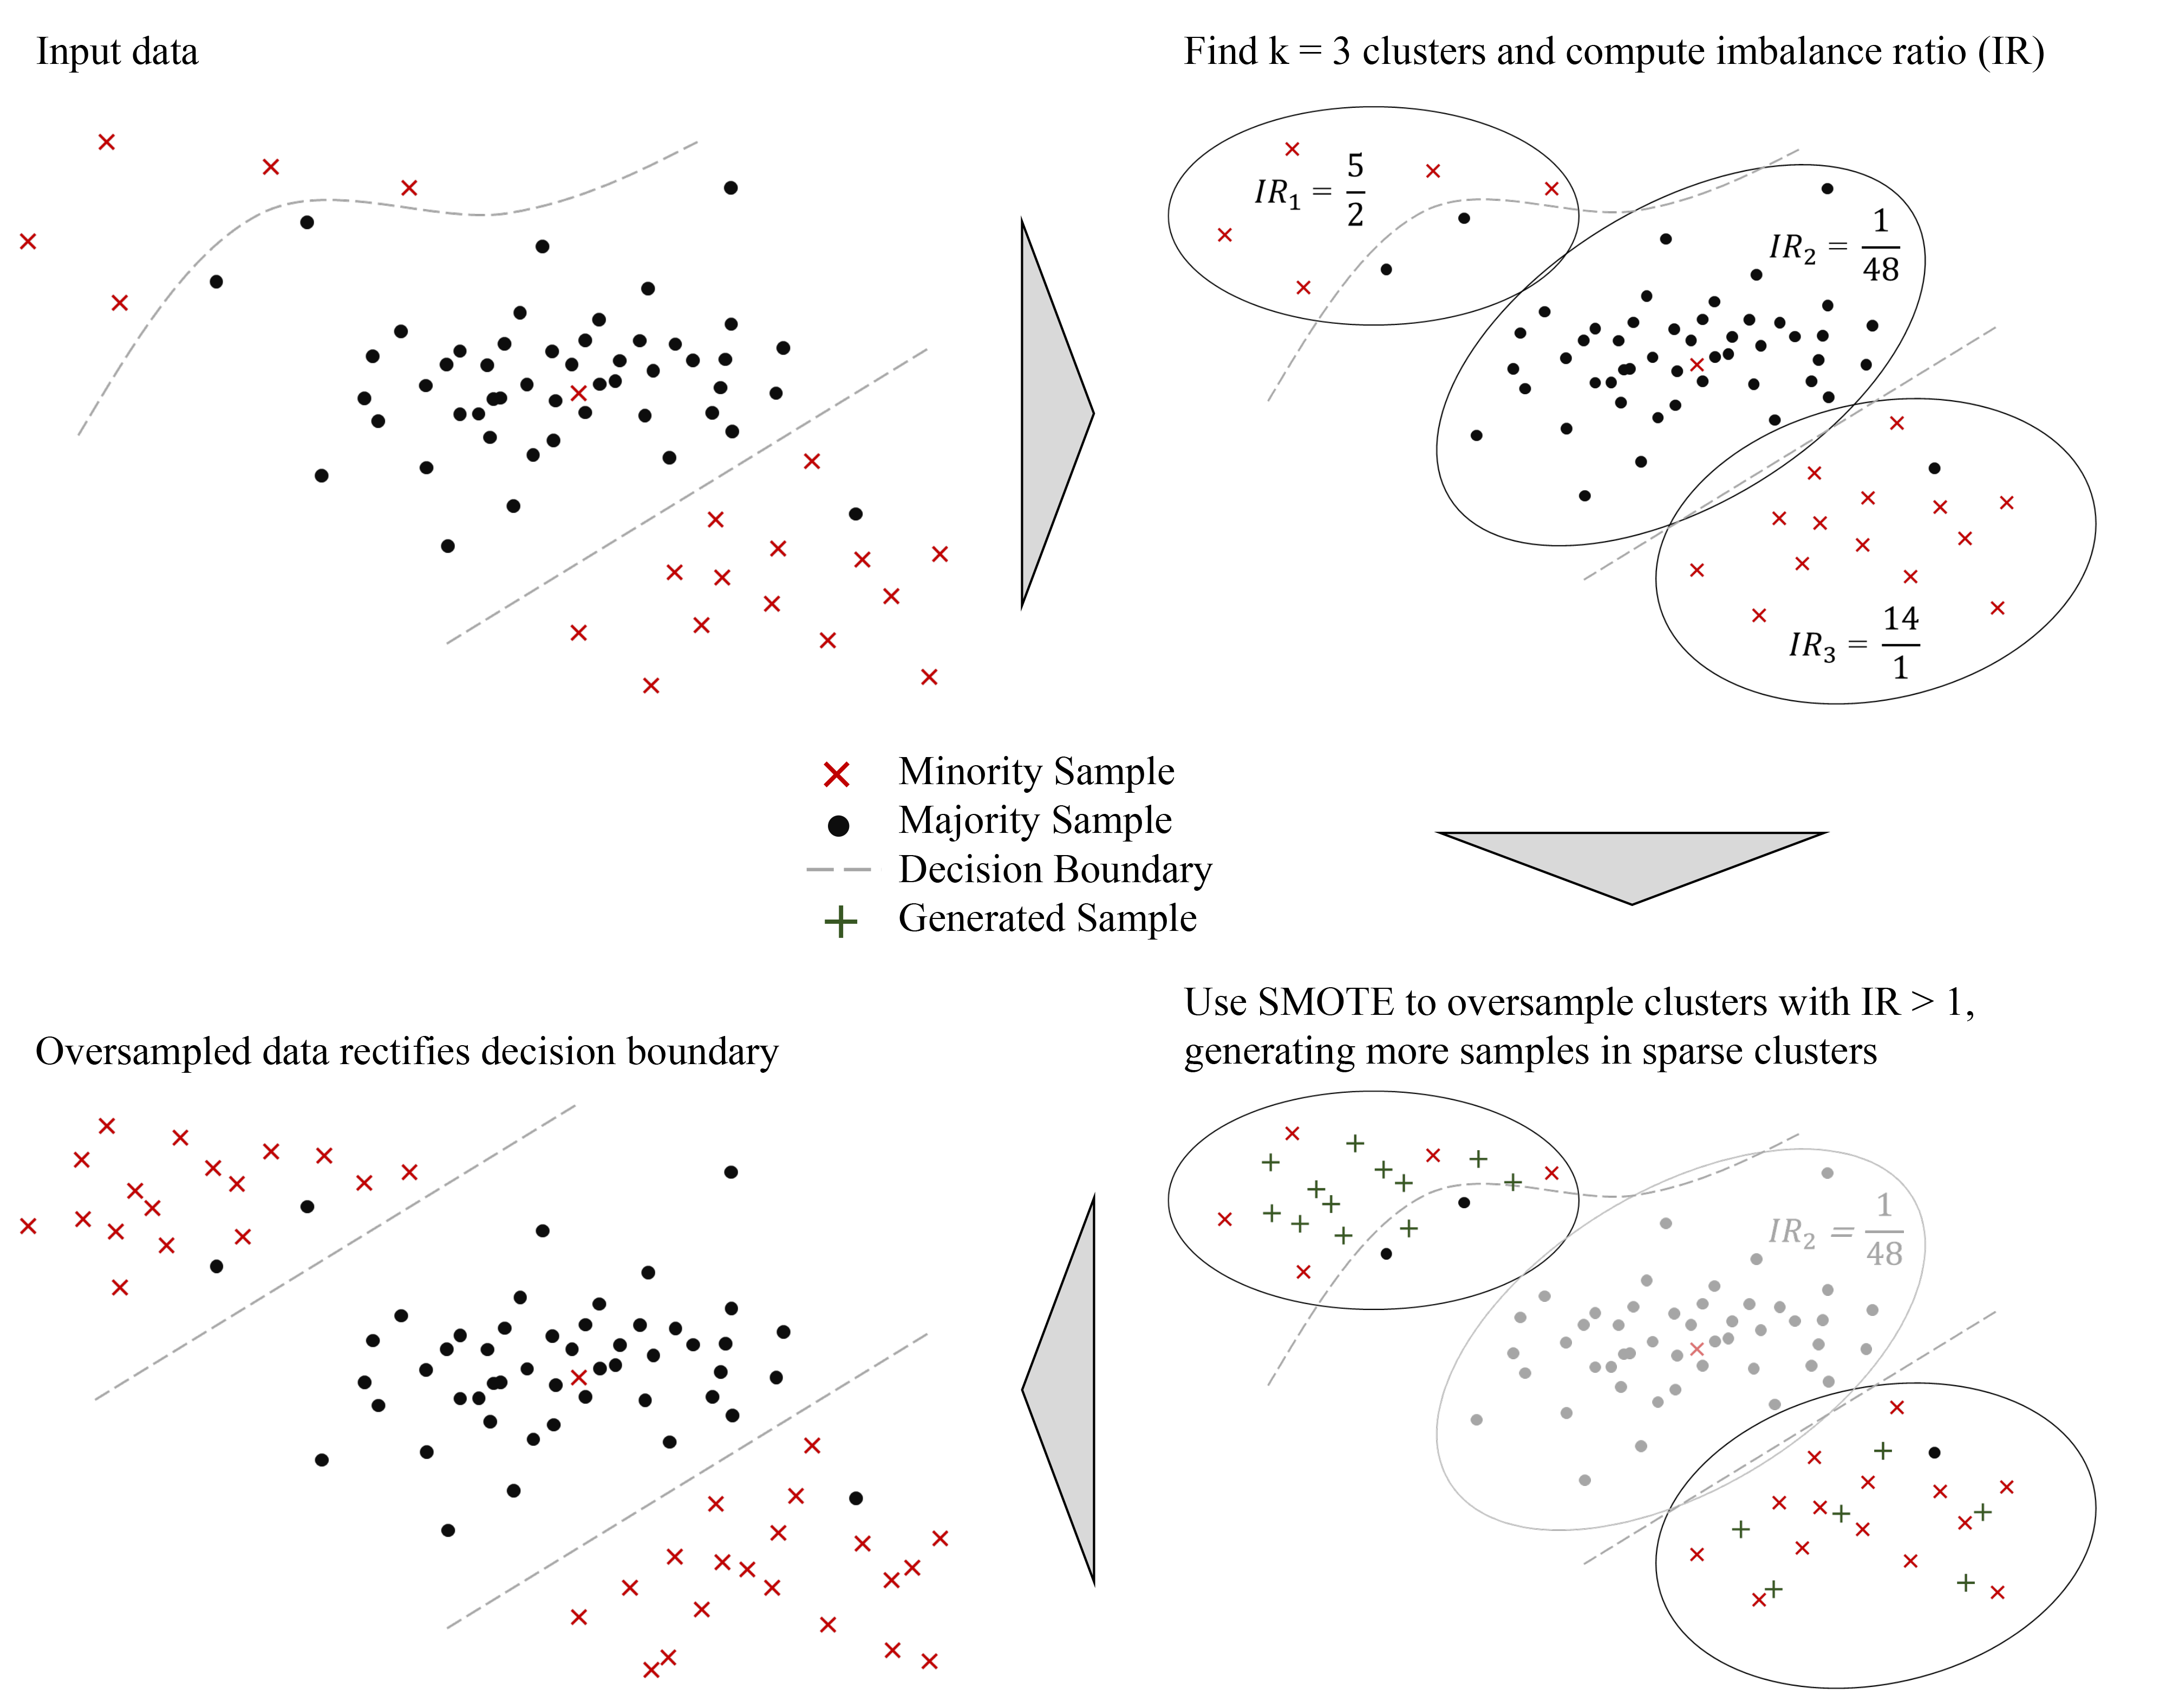
\includegraphics[width=1\textwidth]{../analysis/kmeans-smote-illustration.png}
	\caption[K-means \acs{SMOTE} oversamples safe areas and combats within-class imbalance]
	{K-means \ac{SMOTE} oversamples safe areas and combats within-class
	imbalance\protect\footnotemark}
    \label{fig:kmeans-smote-illustration}
	\end{figure}

	%TODO check that footnote is on correct page
	\footnotetext{The rectification of the decision boundary in the lower 
	left of the image is desired because the two majority samples are considered 
	outliers. The classifier is thus able to induce a simpler rule, which is 
	less error prone.}

	The k-means algorithm is a popular iterative method of finding naturally
	occurring groups in data which can be represented in a Euclidean space. It
	works by iteratively repeating two instructions: First, assign each
	observation to the nearest of $k$ cluster centroids. Second, update the
	position of the centroids so that they are centered between the observations
	assigned to them. The algorithm converges when no more observations are
	reassigned. It is guaranteed to converge to a typically local optimum in a
	finite number of iterations~\citep{MacQueen.1967}. For large datasets where
	k-means may be slow to converge, more efficient implementations could be
	used for the clustering step of the k-means \ac{SMOTE}, such as mini-batch
	k-means as proposed by~\citep{Sculley.2010}. All hyperparameters of k-means
	are also hyperparameters of the proposed algorithm, most notably $k$, the
	number of clusters. Finding an appropriate value for $k$ is important for
	the effectiveness of k-means \ac{SMOTE} as it influences how many minority
	clusters, if any, can be found in the filter step.

	Following the clustering step, the filter step chooses clusters to be
	oversampled and determines how many samples are to be generated in each
	cluster. The motivation of this step is to oversample only clusters
	dominated by the minority class, as applying \ac{SMOTE} inside minority
	areas is safer, i.e. less susceptible to noise generation. Moreover, the
	goal is to achieve a balanced distribution of samples \textit{within} the
	minority class. Therefore, the filter step allocates more generated samples
	to sparse minority clusters than to dense ones.
	
	The selection of clusters for oversampling is based on each cluster's
	proportion of minority and majority instances. By default, any cluster made
	up of at least 50 \% minority samples is selected for oversampling. This
	behavior can be tuned by adjusting the imbalance ratio threshold (or $irt$),
	a hyperparameter of k-means \ac{SMOTE} which defaults to $1$. The imbalance
	ratio of a cluster $c$ is defined as $\frac{\textit{majority count}(c) +
	1}{\textit{minority count}(c) + 1}$. When the imbalance ratio threshold is
	increased, cluster choice is more selective and a higher proportion of
	minority instances is required for a cluster to be selected. On the other
	hand, lowering the threshold loosens the selection criterion, allowing
	clusters with a higher majority proportion to be chosen.

	To determine the distribution of samples to be generated, filtered clusters
	are assigned sampling weights between zero and one. A high sampling weight
	corresponds to a low density of minority samples and yields more generated
	samples. To achieve this, the sampling weight depends on how dense a single
	cluster is compared to how dense all selected clusters are on average. Note
	that when measuring a cluster's density, only the distances among minority
	instances are considered. The computation of the sampling weight may be
	expressed by means of five sub-computations:
	\begin{enumerate}
		\item For each filtered cluster $f$, calculate the Euclidean distance
		matrix, ignoring majority samples.
		\item Compute the mean distance within each cluster by summing all
		non-diagonal elements of the distance matrix, then dividing by the
		number non-diagonal elements.
		\item To obtain a measure of density, divide each cluster's number of
		minority instances by its average minority distance raised to the power
		of the number of features $m$: $density(f) = \frac{\textit{minority
		count}(f)}{\textit{average minority distance}(f)^{m}}$.
		\item Invert the density measure as to get a measure of sparsity, i.e.
		$sparsity(f) = \frac{1}{density(f)}$.
		\item The sampling weight of each cluster is defined as the cluster's
		sparsity factor divided by the sum of all clusters' sparsity factors.
	\end{enumerate}
	 Consequently, the sum of all sampling weights is one. Due to this property,
	 the sampling weight of a cluster can be multiplied by the overall number of
	 samples to be generated to determine the number of samples to be generated
	 in that cluster.

	In the oversampling step of the algorithm, each filtered cluster is
	oversampled using \ac{SMOTE}. For each cluster, the oversampling procedure
	is given all points of the cluster along with the instruction to generate
	$\Vert \textit{sampling weight}(f) \times n \Vert$ samples, where n is the
	overall number of samples to be generated. Per synthetic sample to generate,
	\ac{SMOTE} chooses a random minority observation $\vec{a}$ within the
	cluster, finds a random neighboring minority instance $\vec{b}$ of that
	point and determines a new sample $\vec{x}$ by randomly interpolating
	$\vec{a}$ and $\vec{b}$. In geometric terms, the new point $\vec{x}$ is thus
	placed somewhere along a straight line from $\vec{a}$ to $\vec{b}$. The
	process is repeated until the number of samples to be generated is reached. 
	
	\ac{SMOTE}'s hyperparameter k nearest neighbors, or $knn$, constitutes among
	how many neighboring minority samples of $\vec{a}$ the point $\vec{b}$ is
	randomly selected. This hyperparameter is also used by k-means \ac{SMOTE}.
	Depending on the specific implementation of \ac{SMOTE}, the value of $knn$
	may have to be adjusted downward when a cluster has fewer than $knn + 1$
	minority samples. Once each filtered cluster has been oversampled, all
	generated samples are returned and the oversampling process is completed.

	The proposed method is distinct from related techniques in that it clusters
	the entire dataset regardless of the class label. This unsupervised approach
	enables the discovery of overlapping class regions and may aid the avoidance
	of oversampling in unsafe areas. This is in contrast to cluster-SMOTE, where
	only minority class instances are clustered~\citep{Cieslak.2006} and to the
	aforementioned combination of oversampling and undersampling where both
	classes are clustered separately~\citep{Song.2016}. Another distinguishing
	feature is the unique approach to the distribution of generated samples
	across clusters: sparse minority clusters yield more samples than dense
	ones. The previously presented method cluster-based oversampling, on the
	other hand, distributes samples based on cluster size~\citep{Jo.2004}. Since
	k-means may find clusters of varying density, but typically of the same
	size~\citep{MacQueen.1967, Wu.2010}, distributing samples according to
	cluster density can be assumed to be an effective way to combat within-class
	imbalance. Lastly, the use of \ac{SMOTE} circumvents the problem of
	overfitting, which random oversampling has been shown to encourage.
	

	\begin{algorithm}[htbp] \DontPrintSemicolon \KwIn{$X$ (matrix of
	observations)}
	\kwInMultiline{$y$ (target vector)}
	\kwInMultiline{$n$ (number of samples to be generated)}
	\kwInMultiline{$k$ (number of clusters to be found by k-means)}
	\kwInMultiline{$irt$ (imbalance ratio threshold)}
	\kwInMultiline{$knn$ (number of nearest neighbors considered by \ac{SMOTE})}
	\kwInMultiline{$de$ (exponent used for computation of density; defaults to the 
	number of features in $X$)}
	\Begin{
		\tcp{Step 1: Cluster the input space and filter clusters with more minority 
		instances than majority instances.}
		$clusters \gets kmeans(X)$\; $\textit{filtered clusters} \gets
		\varnothing$\; \For{$c \in clusters $}{$\textit{imbalance ratio} \gets
		\frac{\textit{majority count}(c) + 1}{\textit{minority count}(c) + 1}$\;
		\If{$\textit{imbalance ratio} < irt$}{$\textit{filtered clusters} \gets
		\textit{filtered clusters} \cup \{ c \}$\;}}
		
		\;
		\tcp{Step 2: For each filtered cluster, compute the sampling weight based on its minority density.}
		\For{$f \in \textit{filtered clusters} $}{$\textit{average minority
			distance}(f) \gets mean( \textit{euclidean distances}(f) )$\;
			$\textit{density factor}(f) \gets \frac{\textit{minority
			count}(f)}{\textit{average minority distance}(f)^{de}}$\;
			$\textit{sparsity factor}(f) \gets \frac{1}{\textit{density
			factor}(f)}$} $\textit{sparsity sum} \gets \sum_{f \in
			\textit{filtered clusters}}^{} \textit{sparsity factor}(f)$\;
			$\textit{sampling weight}(f) \gets \frac{\textit{sparsity
			factor}(f)}{\textit{sparsity sum}}$\;

		\;
		\tcp{Step 3: Oversample each filtered cluster using \ac{SMOTE}. The number of samples to 
		be generated is computed using the sampling weight.}
		$\textit{generated samples} \gets \varnothing$\; \For{$f \in
		\textit{filtered clusters} $}{$\textit{number of samples} \gets \Vert n
		\times \textit{sampling weight}(f) \Vert$\; $\textit{generated samples}
		\gets \textit{generated samples} \cup \{\, SMOTE(f,\, \textit{number of
		samples},\, knn) \, \}$\;} \Return{$\textit{generated samples}$}}
	\caption{Proposed method based on k-means and \ac{SMOTE}}
	\end{algorithm}

	\subsection{Limit Cases}
	In the following, it is shown that \ac{SMOTE} and random oversampling can be
	regarded as limit cases of the more general method proposed in this work. In
	k-means \ac{SMOTE}, the input space is clustered using k-means.
	Subsequently, some clusters are selected and then oversampled using
	\ac{SMOTE}. Considering the case where the number of clusters $k$ is equal
	to 1, all observations are grouped in one cluster. For this only cluster to
	be selected as a minority cluster, the imbalance ratio threshold needs to be
	set so that the imbalance ratio of the training data is met. For example, in
	a dataset with 100 minority observations and 10,000 majority observations,
	the imbalance ratio threshold must be greater than or equal to $\frac{10,000
	+ 1}{100 + 1} \approx 99.02$. The single cluster is then selected and
	oversampled using \ac{SMOTE}; since the cluster contains all observations,
	this is equivalent to simply oversampling the original dataset with
	\ac{SMOTE}. Instead of setting the imbalance ratio threshold to the exact
	imbalance ratio of the dataset, it can simply be set to positive infinity.

	If \ac{SMOTE} did not interpolate two different points to generate a new
	sample but performed the random interpolation of one and the same point, the
	result would be a copy of the original point. This behavior could be
	achieved by setting the parameter ``k nearest neighbors'' of \ac{SMOTE} to
	zero if the concrete implementation supports this behavior. As such, random
	oversampling may be regarded as a specific case of \ac{SMOTE}.

	This property of k-means \ac{SMOTE} is of very practical value to its users:
	since it contains both \ac{SMOTE} and random oversampling, a search of
	optimal hyperparameters could include the configurations for those methods.
	As a result, while a better parametrization may be found, the proposed
	method will perform at least as well as the better of both oversamplers. In
	other words, \ac{SMOTE} and random oversampling are fallbacks contained in
	k-means \ac{SMOTE}, which can be resorted to when the proposed method does
	not produce any gain with other parametrizations. \Cref{tab:limit-case}
	summarizes the parameters which may be used to reproduce the behavior of
	both algorithms.
	\begin{table}[!htb]
		\centering
		\rowcolors{2}{gray!10}{white}	
		\begin{tabular}{lrrrrr}
		\toprule
							& $k$ & $irt$    & $knn$ \\
		\midrule
		\ac{SMOTE}          & 1 & $\infty$ &     \\
		Random Oversampling & 1 & $\infty$ & 0  \\
		\bottomrule
		\end{tabular}
		\caption{Limit case configurations}
		\label{tab:limit-case}
	\end{table}

\section{Research Methodology}
\label{sec:research-methodology}
The ultimate purpose of any resampling method is the improvement of
classification results. In other words, a resampling technique is successful if
the resampled data it produces improves the prediction quality of a given
classifier. Therefore, the effectiveness of an oversampling method can only be
assessed indirectly by evaluating a classifier trained on oversampled data. This
proxy measure, i.e. the classifier performance, is only meaningful when compared
with the performance of the same classification algorithm trained on data which
has not been resampled. Multiple oversampling techniques can then be ranked by
evaluating a classifier's performance with respect to each modified training set
produced by the resamplers.

A general concern in classifier evaluation is the bias of evaluating predictions
for previously seen data. Classifiers may perform well when making predictions
for rows of data used during training, but poorly when classifying new data.
This problem is also referred to as overfitting. Oversampling techniques have
been observed to encourage overfitting, which is why this bias should be
carefully avoided during their evaluation. A general approach is to split the
available data into two or more subsets of which only one is used during
training, and another is used to evaluate the classification. The latter is
referred to as the holdout set, unknown data, or test dataset. 

Arbitrarily splitting the data into two sets, however, may introduce additional
biases. One potential issue that arises is that the resulting training set may
not contain certain observations, preventing the algorithm from learning
important concepts. Cross-validation combats this issue by randomly splitting
the data many times, each time training the classifier from scratch using one
portion of the data before measuring its performance on the remaining share of
data. After a number of repetitions, the classifier can be evaluated by
aggregating the results obtained in each iteration. In k-fold cross-validation,
a popular variant of cross-validation, $k$ iterations, called folds, are
performed. During each fold, the test set is one of $k$ equally sized groups.
Each group of observations is used exactly once as a holdout set. K-fold
cross-validation can be repeated many times to avoid potential bias due to
random grouping~\citep{Japkowicz.2013}.

While k-fold cross validation typically avoids the most important biases in
classification tasks, it might distort the class distributions when randomly
sampling from a class-imbalanced dataset. In the presence of extreme skews,
there may even be iterations where the test set contains no instances of the
minority class, in which case classifier evaluation would be ill-defined or
potentially strongly biased. A simple and common approach to this problem is to
use stratified cross-validation, where instead of sampling completely at random,
the original class distribution is preserved in each
fold~\citep{Japkowicz.2013}.

	\subsection{Metrics}
	Of the various assessment metrics traditionally used to evaluate classifier
	performance, not all are suitable when the class distribution is not
	uniform. However, there are metrics which have been employed or developed
	specifically to cope with imbalanced data.

	Classification assessment metrics compare the true class membership of each
	observation with the prediction of the classifier. To illustrate the
	alignment of predictions with the true distribution, a confusion matrix
	(\cref{fig:confusion-matrix}) can be constructed.	Possibly deriving from
	medical diagnoses, a positive observation is a rare case and belongs to the
	minority class. The majority class is considered
	negative~\citep{Japkowicz.2013}.

	\begin{figure}[ht]
	\centering
	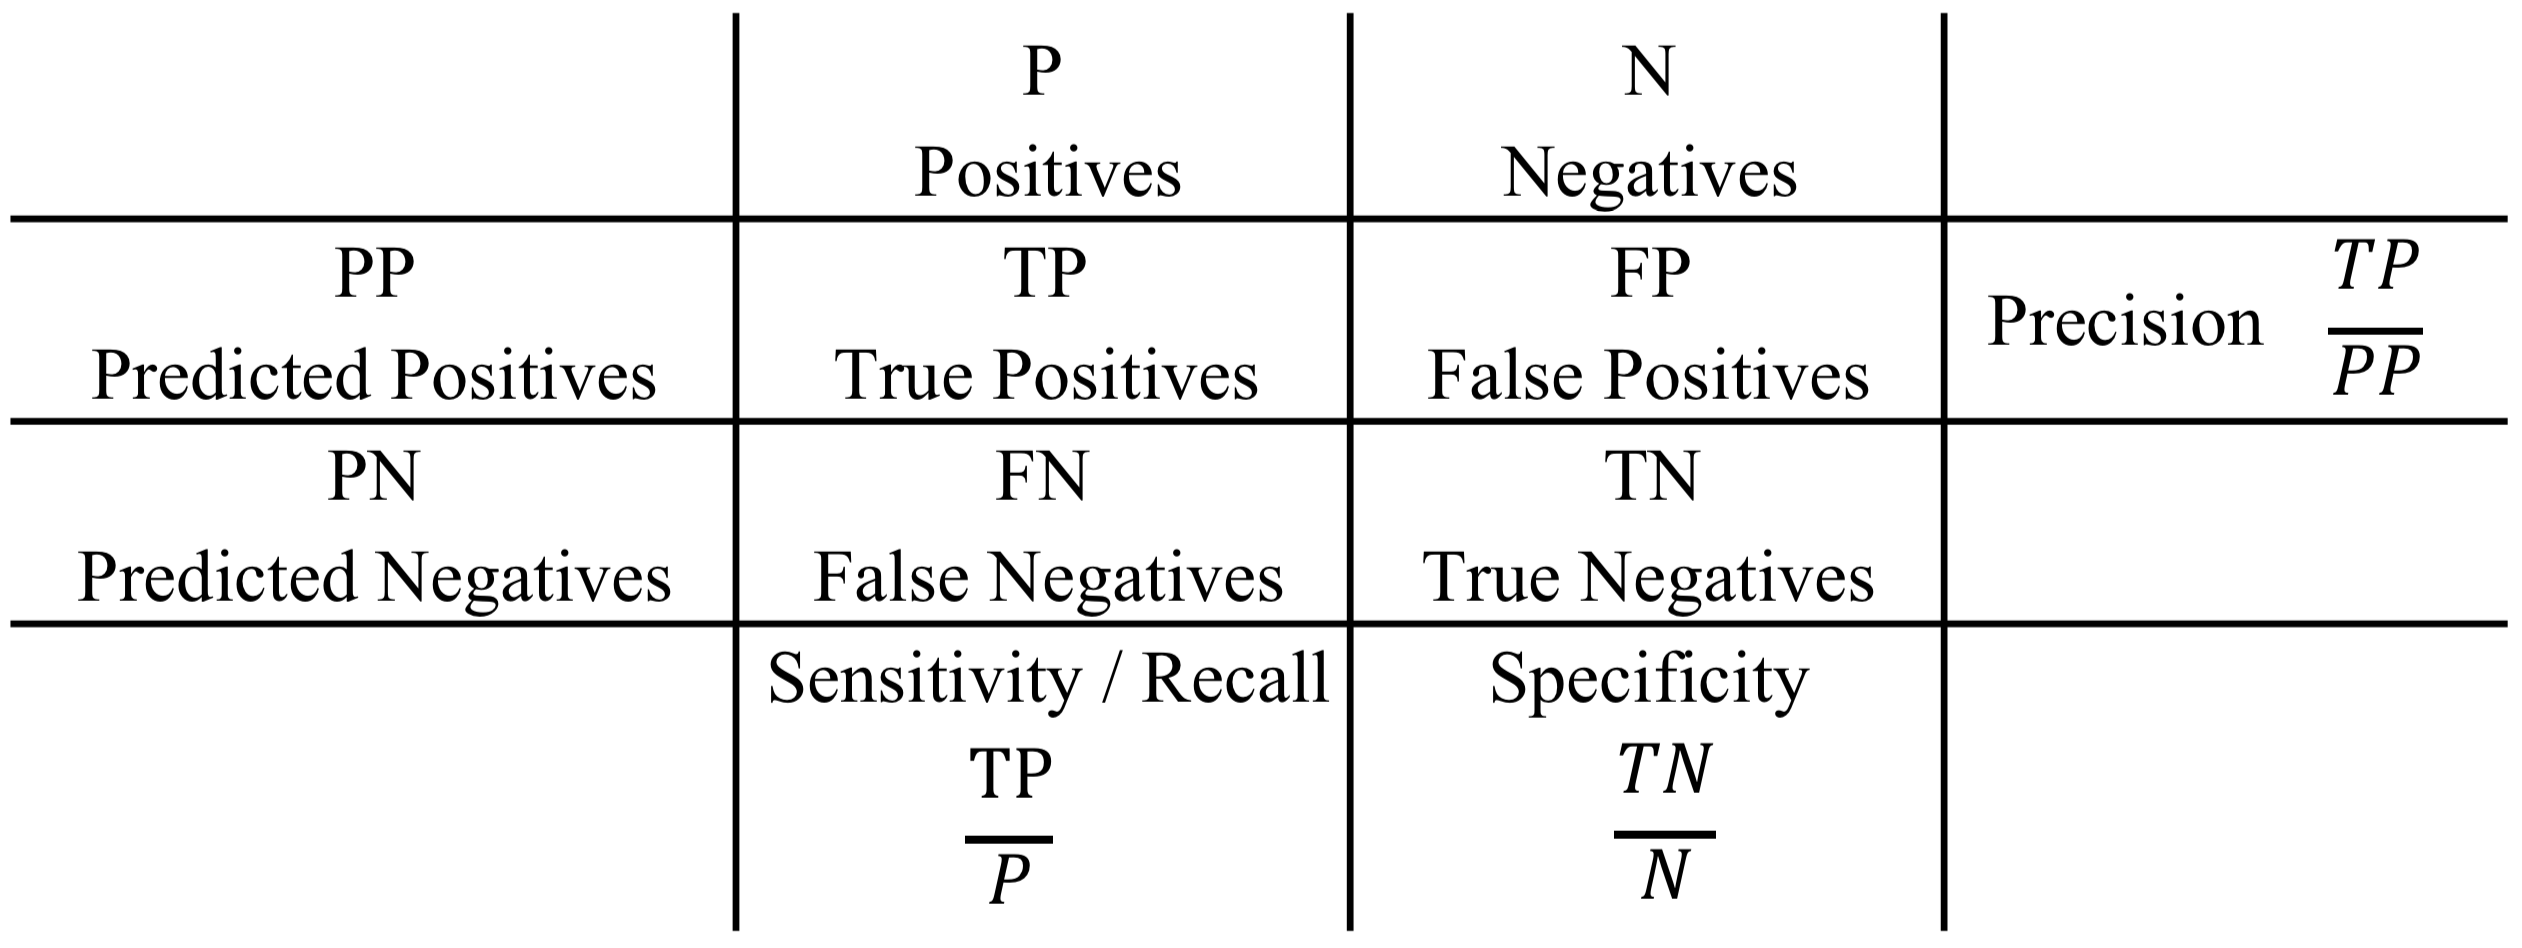
\includegraphics[width=0.6\textwidth]{../analysis/confusion-matrix.png}
	\caption{Confusion matrix}
    \label{fig:confusion-matrix}
	\end{figure}
	
	When evaluating a single classifier in the context of a finite dataset with
	fixed imbalance ratio, the confusion matrix provides all necessary
	information to assess the classification quality. However, when comparing
	different classifiers or evaluating a single classifier in variable
	environments, the absolute values of the confusion matrix are non-trivial.

	The most common metrics for classification problems are accuracy and its
	inverse, error rate.
	\begin{equation}
	Accuracy = \frac{TP + TN}{P + N};\ \textit{Error Rate} = 1 - Accuracy
	\end{equation}
	These metrics show a bias toward the majority class in imbalanced datasets.
	For example, a naive classifier which predicts all observations as negative
	would achieve 99\% accuracy in a dataset where only 1\% of instances are
	positive. While such high accuracy suggests an effective classifier, the
	metric obscures the fact that not a single minority instance was predicted
	correctly~\citep{He.2009}.

	 Sensitivity, also referred to as recall or true positive rate, explains the
	 prediction accuracy among minority class instances. It answers the question
	 ``How many minority instances were correctly classified as such?''
	 Specificity answers the same question for the majority class. Precision is
	 the rate of correct predictions among all instances predicted to belong to
	 the minority class. It indicates how many of the positive predictions are
	 correct~\citep{He.2009}.

	 The F1-score, or F-measure, is the (often weighted) harmonic mean of
	 precision and recall. In other terms, the indicator rates both the
	 completeness and exactness of positive
	 predictions~\citep{He.2009,Japkowicz.2013}.
	 
	\begin{equation}
	F1 = \frac{(1 + \alpha) \times (sensitivity \times precision)}{sensitivity + \alpha \times precision} 
	= \frac{(1 + \alpha) \times (\frac{TP}{P} \times \frac{TP}{PP})}{\frac{TP}{P} + \alpha \times \frac{TP}{PP} }
	\end{equation}

	The geometric mean score, also referred to as g-mean or g-measure, is
	defined as the geometric mean of sensitivity and specificity. The two
	components can be regarded as per-class accuracy. The g-measure aggregates
	both metrics into a single value in $[0,1]$, assigning equal importance to
	both~\citep{He.2009,Japkowicz.2013}.
	
	\begin{equation}
	g\mhyphen mean = \sqrt{sensitivity \times specificity} 
	= \sqrt{\frac{TP}{P} \times \frac{TN}{N}}
	\end{equation}

	\acp{PR} diagrams plot the precision of a classifier as a function of its
	minority accuracy. Classifiers outputting class membership confidences (i.e.
	continuous values in $[0,1]$) can be plotted as multiple points in discrete
	intervals, resulting in a \ac{PR} curve. Commonly, the \ac{AUPRC} is
	computed as a single numeric performance
	metric~\citep{He.2009,Japkowicz.2013}.
	
	The choice of metric depends to a great extent on the goal their user seeks
	to achieve. In certain practical tasks, one specific aspect of
	classification may be more important than another (e.g. in medical
	diagnoses, false negatives are much more critical than false positives).
	However, to determine a general ranking among oversamplers, no such focus
	should be placed. Therefore, the following unweighted metrics are chosen for
	the evaluation.
    \begin{itemize}
    	\item g-mean
        \item F1-score
		\item \ac{AUPRC}
	\end{itemize}
   
	\subsection{Oversamplers}
	The following list enumerates the oversamplers used as a benchmark for the
	evaluation of the proposed method, along with the set of hyperparameters
	used for each. The optimal imbalance ratio is not obvious and has been
	discussed by other
	researchers~\citep{Provost.2000,Estabrooks.2004,Chawla.2008}. This work aims
	at creating comparability among oversamplers; consequently, it is most
	important that oversamplers achieve the same imbalance ratio. Therefore, all
	oversampling methods were parametrized to generate as many instances as
	necessary so that minority and majority classes count the same number of
	samples.
	\begin{itemize}
		\item random oversampling
		\item SMOTE
		\begin{itemize}
			\item $knn \in \{3, 5, 20\}$
		\end{itemize}
		\item borderline-SMOTE1
		\begin{itemize}
			\item $knn \in \{3, 5, 20\}$
		\end{itemize}
		\item borderline-SMOTE2
		\begin{itemize}
			\item $knn \in \{3, 5, 20\}$
		\end{itemize}
		\item k-means SMOTE
		\begin{itemize}
			\item $k \in \{2, 20, 50, 100, 250, 500\}$
			\item $knn \in \{3, 5, 20, \infty\}$
			\item $irt \in \{1, \infty\}$
			\item $de \in \{0, 2, \textit{number of features}\}$
		\end{itemize}
		\item no oversampling
	\end{itemize}

	\subsection{Classifiers}
	For the evaluation of the various oversampling methods, several different
	classifiers are chosen to ensure that the results obtained can be
	generalized and are not constrained to the usage of a specific classifier.
	The choice of classifiers is further motivated by the number of
	hyperparameters: classification algorithms with few or no hyperparameters
	are less likely to bias results due to their specific configuration.

	\acp{LR} is a generalized linear model which can be used for binary
	classification. Fitting the model is an optimization problem which can be
	solved using simple optimizers which require no hyperparameters to be
	set~\citep{McCullagh.1984}. Consequently, results achieved by \ac{LR} are
	easily reproducible, while also constituting a baseline for more
	sophisticated approaches.

	Another classification algorithm referred to as \ac{KNN} assigns an
	observation to the class most of its nearest neighbors belong to. How many
	neighbors are considered is determined by the method's
	hyperparameter~$k$~\citep{Fix.1951}.

	Finally, gradient boosting over decision trees, or simply \ac{GBM}, is an
	ensemble technique used for classification. In the case of binary
	classification, one shallow decision tree is induced at each stage of the
	algorithm. Each tree is fitted to observations which could not be correctly
	classified by decision trees of previous stages. Predictions of \ac{GBM} are
	made by majority vote of all trees. In this way, the algorithm combines
	several simple models (referred to as weak learners) to create one effective
	classifier. The number of decision trees to generate, which in binary
	classification is equal to the number of stages, is a hyperparameter of the
	algorithm~\citep{Friedman.2001}. 

	As further explained in \cref{sec:experimental-framework}, various
	combinations of hyperparameters are tested for each classifier. All
	classifiers are used as implemented in the Python library
	scikit-learn~\citep{Pedregosa.2011} with default parameters unless stated
	otherwise. The following list enumerates the classifiers used in this study
	along with a set of values for their respective hyperparameters.
	\begin{itemize}
		\item \ac{LR}
		\item \ac{KNN}
		\begin{itemize}
            \item $k \in \{3, 5, 8\}$
		\end{itemize}
		\item \ac{GBM}
		\begin{itemize}
            \item $\textit{number of trees} \in \{50, 100, 200\}$
		\end{itemize}
	\end{itemize}

	\subsection{Datasets}
    \label{sec:datasets}
	To evaluate k-means \ac{SMOTE}, 12 imbalanced datasets from the UCI Machine
	Learning Repository~\citep{Lichman.2013} are used. Those datasets containing
	more than two classes were binarized using a one-versus-rest approach,
	labeling the smallest class as the minority and merging all other samples
	into one class. In order to generate additional datasets with even higher
	imbalance ratios, each of the aforementioned datasets was randomly
	undersampled to generate up to six additional datasets. The imbalance ratio
	of each dataset was increased approximately by multiplication factors of 2,
	4, 6, 10, 15 and 20, but only if a given factor did not reduce a dataset's
	total number of minority samples to less than eight. Furthermore, 19
	imbalanced datasets were selected from from the KEEL repository
	\cite{Alcala-fdez.2011}. Lastly, the Python library
	scikit-learn~\citep{Pedregosa.2011} was used to generate ten variations of
	the artificial "MADELON" dataset, which poses a difficult binary
	classification problem~\citep{Guyon.2003}.

	\begin{table}[!htb]
		\rowcolors{2}{gray!10}{white}	
		\begin{tabular}{lrrrrr}
			\toprule
				Dataset &  \# features &  \# samples &  \# minority samples &  \# majority samples &  imbalance ratio \\
			\midrule
				breast\_tissue &              9 &             106 &                       36 &                       70 &             1.94 \\
				ecoli &              7 &             336 &                       52 &                      284 &             5.46 \\
				glass &              9 &             214 &                       70 &                      144 &             2.06 \\
				haberman &              3 &             306 &                       81 &                      225 &             2.78 \\
				heart &             13 &             270 &                      120 &                      150 &             1.25 \\
					iris &              4 &             150 &                       50 &                      100 &             2.00 \\
				libra &             90 &             360 &                       72 &                      288 &             4.00 \\
				liver\_disorders &              6 &             345 &                      145 &                      200 &             1.38 \\
					pima &              8 &             768 &                      268 &                      500 &             1.87 \\
				segment &             16 &            2310 &                      330 &                     1980 &             6.00 \\
				vehicle &             18 &             846 &                      199 &                      647 &             3.25 \\
				wine &             13 &             178 &                       71 &                      107 &             1.51 \\
			\midrule
				new-thyroid1 &              5 &             215 &                       35 &                      180 &             5.14 \\	
				new-thyroid2 &              5 &             215 &                       35 &                      180 &             5.14 \\
				cleveland-0 &             13 &             173 &                       13 &                      160 &            12.31 \\
				dermatology-6 &             34 &             358 &                       20 &                      338 &            16.90 \\
				led7digit &              7 &             443 &                       37 &                      406 &            10.97 \\
				page-blocks0 &             10 &            5472 &                      559 &                     4913 &             8.79 \\
				page-blocks-1-3 &             10 &             472 &                       28 &                      444 &            15.86 \\
				vowel0 &             13 &             988 &                       90 &                      898 &             9.98 \\
				yeast1 &              8 &            1484 &                      429 &                     1055 &             2.46 \\
				yeast2 &              8 &             514 &                       51 &                      463 &             9.08 \\
				yeast3 &              8 &            1484 &                      163 &                     1321 &             8.10 \\
				yeast4 &              8 &            1484 &                       51 &                     1433 &            28.10 \\
				yeast5 &              8 &            1484 &                       44 &                     1440 &            32.73 \\
				yeast-0-2-5-6 &              8 &            1004 &                       99 &                      905 &             9.14 \\
				yeast-0-2-5-7-9 &              8 &            1004 &                       99 &                      905 &             9.14 \\
				yeast-0-3-5-9 &              8 &             506 &                       50 &                      456 &             9.12 \\
				yeast-0-5-6-7-9 &              8 &             528 &                       51 &                      477 &             9.35 \\
				yeast-1-2-8-9 &              8 &             947 &                       30 &                      917 &            30.57 \\
				yeast-2\_vs\_4 &              8 &             514 &                       51 &                      463 &             9.08 \\
				yeast-2\_vs\_8 &              8 &             482 &                       20 &                      462 &            23.10 \\
			\midrule
				simulated1 &             20 &            4000 &                       25 &                     3975 &           159.00 \\
				simulated2 &             20 &            4000 &                       23 &                     3977 &           172.91 \\
				simulated3 &             20 &            4000 &                       23 &                     3977 &           172.91 \\
				simulated4 &             20 &            4000 &                       26 &                     3974 &           152.85 \\
				simulated5 &             20 &            4000 &                       23 &                     3977 &           172.91 \\
				simulated6 &            200 &            3000 &                       20 &                     2980 &           149.00 \\
				simulated7 &            200 &            3000 &                       19 &                     2981 &           156.89 \\
				simulated8 &            200 &            3000 &                       15 &                     2985 &           199.00 \\
				simulated9 &            200 &            3000 &                       13 &                     2987 &           229.77 \\
				simulated10 &            200 &            3000 &                       22 &                     2978 &           135.36 \\
			\bottomrule
			\end{tabular}
		\caption{Summary of datasets used to evaluate and compare the proposed method 
		(split by data source; top: UCI, middle: KEEL, bottom: generated; some names shortened)}
		\label{tab:datasets}
	\end{table}
	
	\Cref{tab:datasets} lists the datasets used to evaluate the proposed method,
	along with important characteristics. The artificial datasets are referred
	to as simulated. Undersampled versions of the original datasets are omitted
	from the table; in the figures presented in \cref{sec:experimental-results},
	the factor used for undersampling is appended to the dataset names. All
	modified and simulated datasets used in the study are made available at
	\url{https://github.com/felix-last/evaluate-kmeans-smote/releases/download/v0.0.1/uci_extended.tar.gz}
	for the purpose of reproducibility.


	Additionally, in order to demonstrate the properties of k-means \ac{SMOTE},
	five two-dimensional binary class datasets are introduced. Three of those
	datasets, which were created for the purpose of this work, consist of
	observations in three partially noisy clusters. They are referred to as
	datasets A, B and C and can be found at
	\url{https://github.com/felix-last/evaluate-kmeans-smote/releases/download/v0.0.2/toy_datasets.tar.gz}.
	The other two toy datasets were created using the ``make\textunderscore
	circles'' and ``make\textunderscore moons'' functions of scikit-learn with a
	noise factor of $0.3$. 750 samples of each class were generated, before one
	class was randomly undersampled to 200 observations.

	\subsection{Experimental Framework}
	\label{sec:experimental-framework}
	To evaluate the proposed method, the oversamplers, metrics, datasets, and
	classifiers discussed in this section are used. Results are obtained by
	repeating 5-fold cross-validation five times. For each dataset, every metric
	is computed by averaging their values across runs. In addition to the
	arithmetic mean, the standard deviation is calculated.

	To achieve optimal results for all classifiers and oversamplers, a grid
	search procedure is used. For this purpose, each classifier and each
	oversampler specifies a set of possible values for every hyperparameter.
	Subsequently, all possible combinations of an algorithm's hyperparameters
	are generated and the algorithm is executed once for each combination. All
	metrics are used to score all resulting classifications, and the best value
	obtained for each metric is saved.

	To illustrate this process, consider an example with one oversampler and one
	classifier. The following list shows each algorithm with several
	combinations for each parameter.
	\begin{itemize}
		\item \ac{SMOTE}
		\begin{itemize}
			\item $knn \in \{3, 6\}$
		\end{itemize}
		\item \ac{GBM}
		\begin{itemize}
			\item $\textit{number of trees} \in \{10, 50\}$
		\end{itemize}
	\end{itemize}
	The oversampling method \ac{SMOTE} is run two times, generating two
	different sets of training data. For each set of training data, the
	classifier \ac{LR} is executed twice. Therefore, the classifier will be
	executed four times. The possible combinations are:
	\begin{itemize}
		\item $knn = 3, \textit{number of trees} = 10$
		\item $knn = 3, \textit{number of trees} = 50$
		\item $knn = 6, \textit{number of trees} = 10$
		\item $knn = 6, \textit{number of trees} = 50$
	\end{itemize}
	If two metrics are used for scoring, both metrics score all four runs; the
	best result is saved. Note that one metric may find that the combination
	$knn = 3, \textit{number of trees} = 10$ is best, while a different
	combination might be best considering another metric. In this way, each
	oversampler and classifier combination is given the chance to optimize for
	each metric.
    
\section{Experimental Results}
\label{sec:experimental-results}

Following recommendations of \citet{Demsar.2006} for evaluating classifier
performance across multiple datasets, obtained scores are not compared directly,
but instead ordered to derive a ranking. To adapt the method for the evaluation
of oversampling techniques, oversamplers are ranked in place of classification
algorithms. Combined with the Friedman~test~\citep{Friedman.1937} and
Holm's~method~\citep{Holm.1979}, this evaluation method is also used by other
authors working on the topic of imbalanced
classification~\citep{Cieslak.2012,Rivera.2017,Galar.2016}.

\begin{figure}[!htb]
\centering
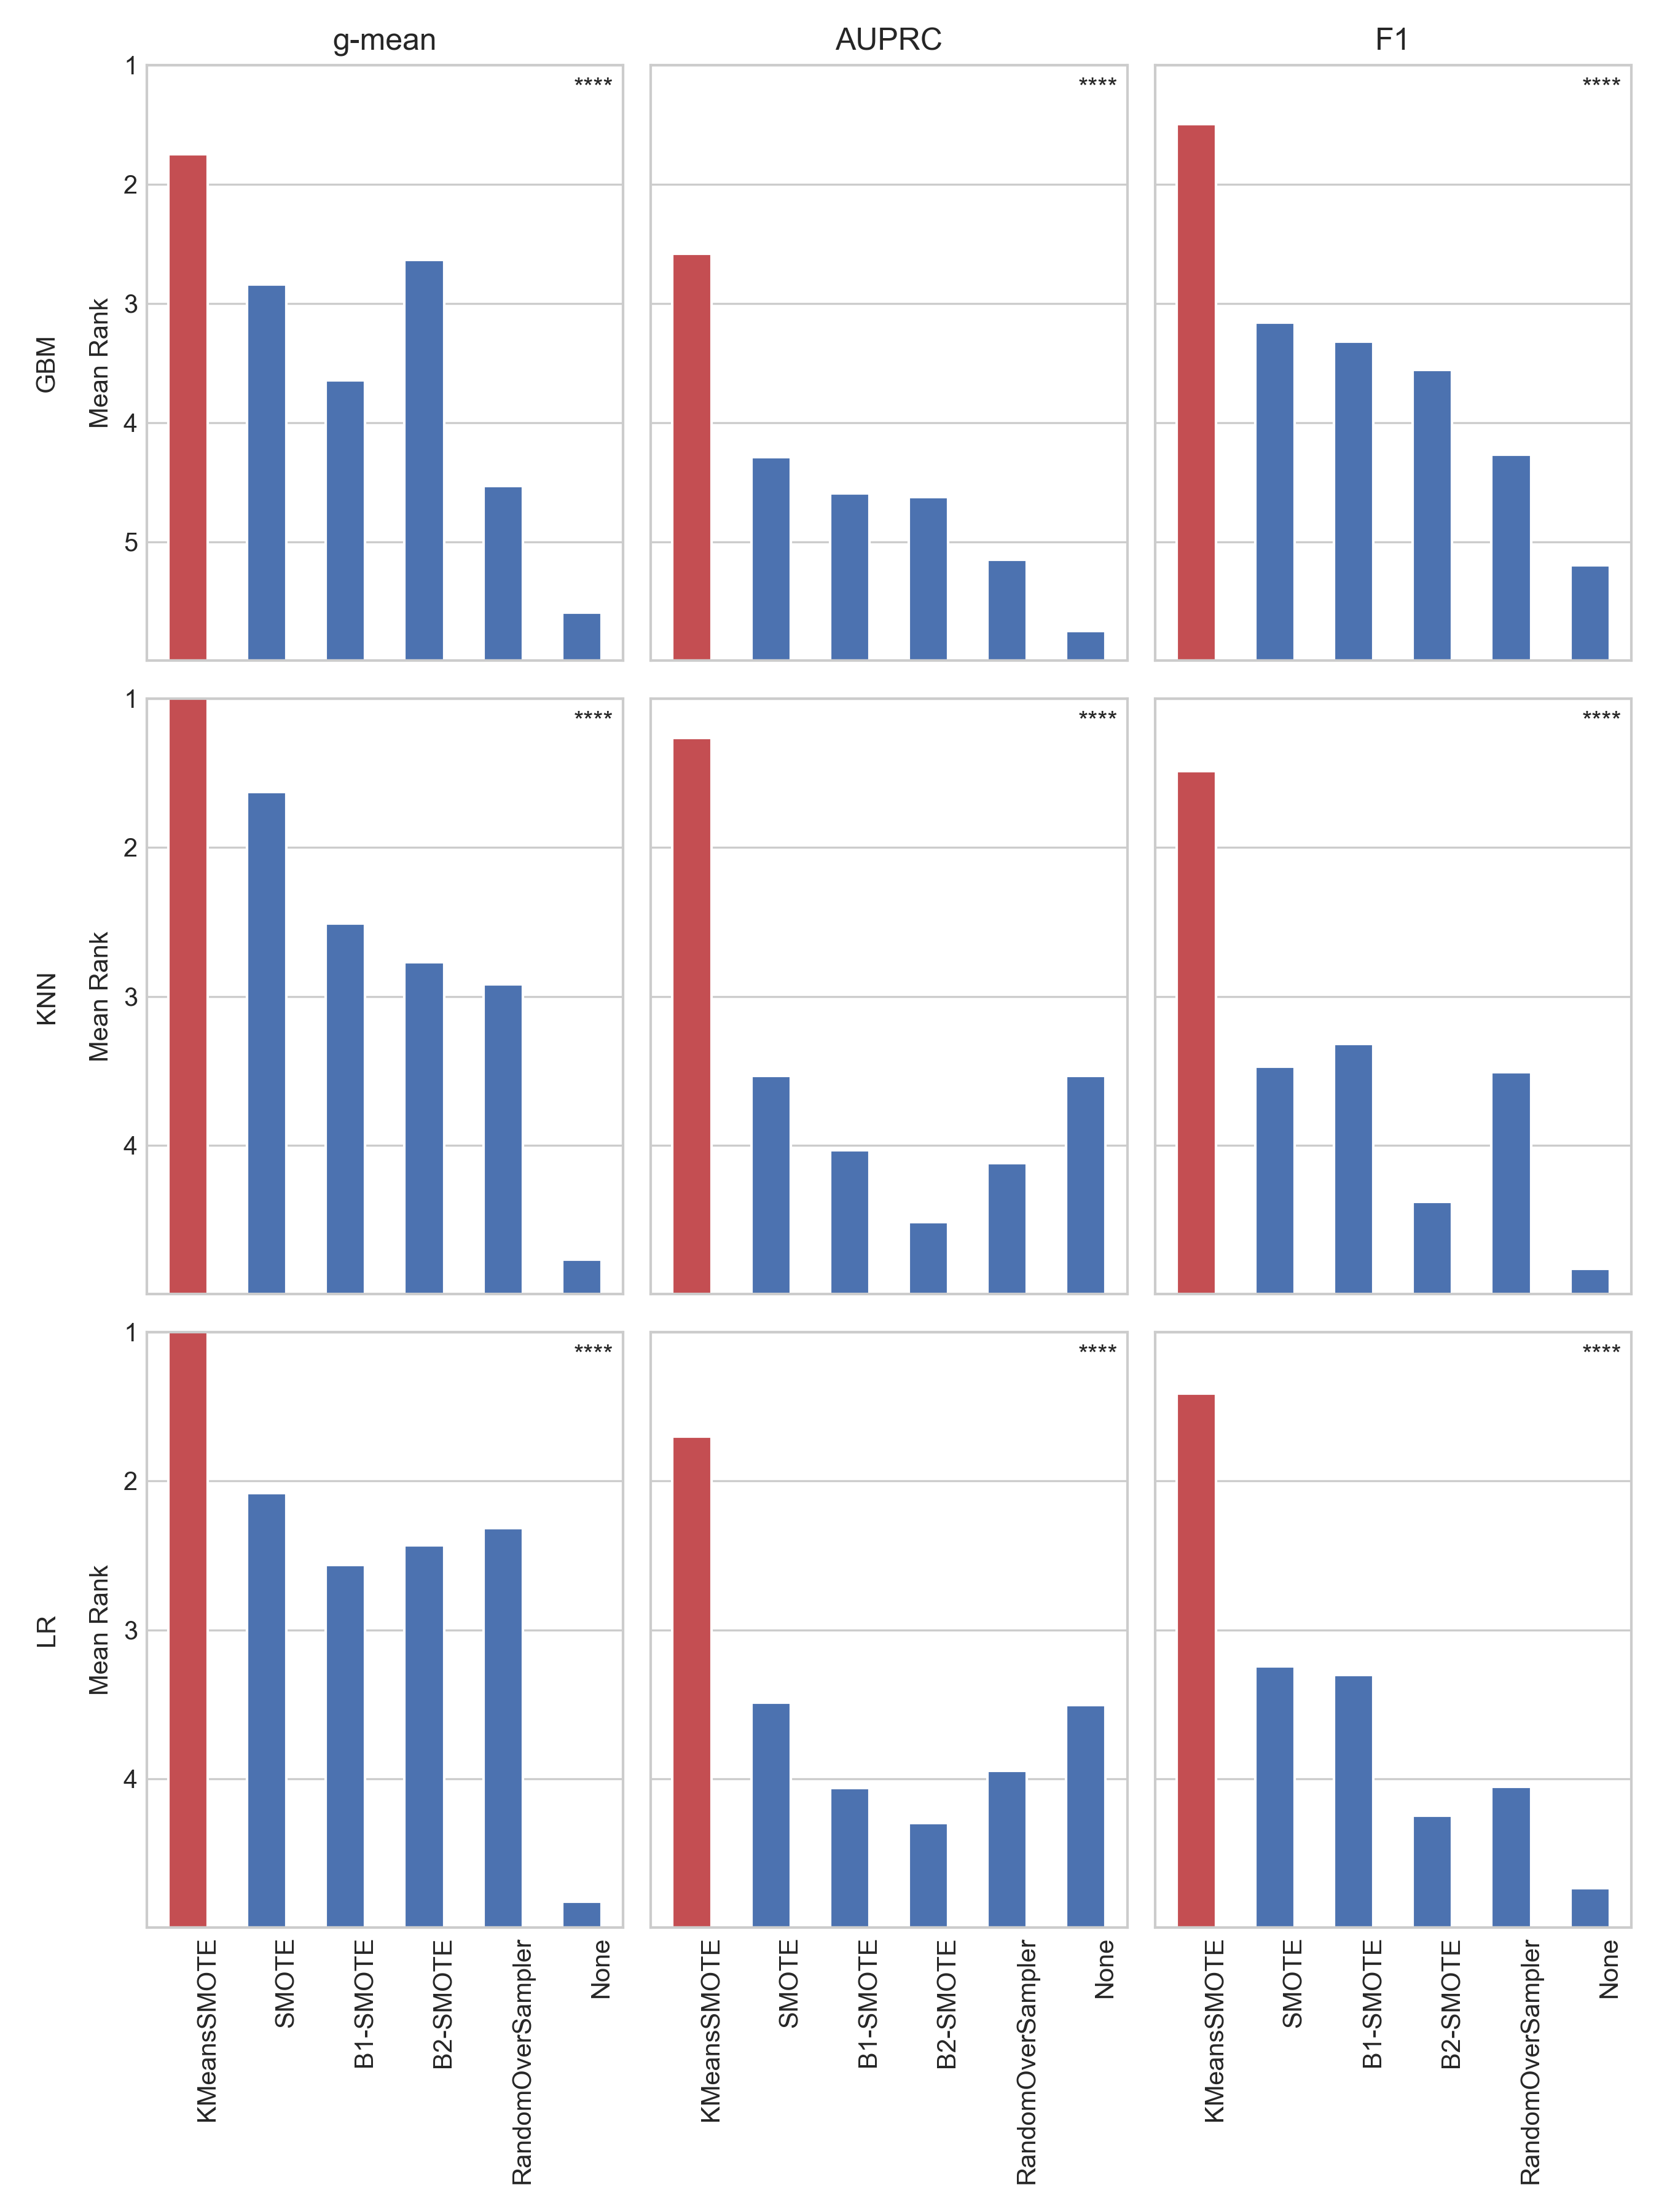
\includegraphics[width=0.75\textwidth]{../analysis/ranking.png}
\caption[Mean ranking of evaluated oversamplers for different classifiers and metrics]
{Mean ranking (best: 1; worst: 6) of evaluated oversamplers for different classifiers and metrics}
\label{fig:ranking}
\end{figure}

\begin{table}[!htb]
	\centering
	\rowcolors{2}{gray!10}{white}	
	\begin{tabular}{lrrrrrr}
	\toprule
	\multicolumn{1}{c}{Classifier} &
	\multicolumn{2}{c}{GBM} &
	\multicolumn{2}{c}{KNN} &
	\multicolumn{2}{c}{LR}\\
	\cmidrule(lr){2-3}
	\cmidrule(lr){4-5}
	\cmidrule(lr){5-7}
	$\alpha _{0.05}$				&       Oversampler & p-value &       Oversampler & p-value &       Oversampler & p-value \\
	% Metric & {} &               &            &               &            &               &            \\
	\midrule
	\multicolumn{2}{l}{Metric: AUPRC} & & & & & \\
	$0.01$        		& None              & $1.47E-30$ & B2-SMOTE          & $4.58E-32$ & B2-SMOTE          & $4.36E-21$ \\
	$0.0125$      		& Random O. & $9.18E-21$ & Random O. & $3.47E-25$ & B1-SMOTE          & $9.58E-18$ \\
	$0.01\overline{66}$ 	& B2-SMOTE          & $8.56E-14$ & B1-SMOTE          & $8.90E-24$ & Random O. & $3.17E-16$ \\
	$0.025$       		& B1-SMOTE          & $2.07E-13$ & None              & $1.40E-16$ & None              & $4.07E-11$ \\
	$0.05$        		& SMOTE             & $3.61E-10$ & SMOTE             & $1.40E-16$ & SMOTE             & $6.03E-11$ \\
	\multicolumn{2}{l}{Metric: F1} & & & & & \\
	$0.01$        		& None              & $5.73E-41$ & None              & $1.03E-33$ & None              & $2.12E-33$ \\
	$0.0125$      		& Random O. & $7.29E-24$ & B2-SMOTE          & $1.00E-25$ & B2-SMOTE          & $7.88E-25$ \\
	$0.01\overline{66}$ 	& B2-SMOTE          & $4.71E-14$ & Random O. & $1.55E-13$ & Random O. & $7.94E-22$ \\
	$0.025$       		& B1-SMOTE          & $2.40E-11$ & SMOTE             & $4.29E-13$ & B1-SMOTE          & $4.72E-12$ \\
	$0.05$        		& SMOTE             & $9.71E-10$ & B1-SMOTE          & $2.10E-11$ & SMOTE             & $1.84E-11$ \\
	\multicolumn{2}{l}{Metric: g-mean} & & & & & \\
	$0.01$        		& None              & $4.98E-44$    & None              & $4.73E-56$ & None              & $1.39E-48$ \\
	$0.0125$      		& Random O. & $4.88E-24$    & Random O. & $6.92E-20$ & B1-SMOTE          & $5.29E-11$ \\
	$0.01\overline{66}$ 	& B1-SMOTE          & $3.58E-12$    & B2-SMOTE          & $8.07E-18$ & B2-SMOTE          & $1.10E-09$ \\
	$0.025$       		& SMOTE             & $4.03E-05$    & B1-SMOTE          & $1.63E-14$ & Random O. & $1.30E-08$ \\
	$0.05$        		& B2-SMOTE          & $6.65E-04$ & SMOTE             & $5.46E-06$ & SMOTE             & $1.21E-06$ \\
	\bottomrule
	\end{tabular}
	\caption{Results of Holm's test with k-means \ac{SMOTE} as the control method}
	\label{tab:holm}
\end{table}

To derive the rank order, cross-validated scores are used, assigning rank one to
the best performing and rank six to the worst performing technique. This results
in different rankings for each of five experiment repetitions, again partitioned
by dataset, metric, and classifier. To aggregate the various rankings, each
method's assigned rank is averaged across datasets and experiment repetitions.
Consequently, a method's mean rank is a real number in the interval $[1.0,6.0]$.
The mean ranking results for each combination of metric and classifier are shown
in \cref{fig:ranking}.

Testing the null hypothesis that differences in terms of rank among oversamplers
are merely a matter of chance, the Friedman~test determines the statistical
significance of the derived mean ranking. The test is chosen because it does not
assume normality of the obtained scores. At a significance level of $\alpha =
0.05$, the null hypothesis is rejected for all evaluated classifiers and
evaluation metrics. Therefore, a post-hoc test is applied. Holm's step-down
procedure is applied with the proposed method as the control method. The
procedure corrects the significance level downwards to account for multiple
testing. The null hypothesis in each pair-wise comparison of the control method
and another oversampler is that the control method does not perform better than
the other method. Table \ref{tab:holm} shows the results of the Holm's test for
all evaluated metrics and classifiers. The null hypothesis is rejected for all
oversamplers at a significance level of $\alpha = 0.05$, indicating that the
proposed method outperforms all other methods.

The mean ranking shows that the proposed method outperforms other methods with
regard to all evaluation metrics. Notably, the technique's superiority can be
observed independently of the classifier. In eight out of nine cases, k-means
\ac{SMOTE} achieves a mean rank better than two, whilst still better than three
in the remaining case. Furthermore, k-means \ac{SMOTE} is the only technique
with a mean ranking better than three with respect to F1 score and \ac{AUPRC},
boosting classification results when other oversamplers tie or accomplish a
similar rank as no oversampling.

Generally, it can be observed that - aside from the proposed method -
\ac{SMOTE}, borderline-\ac{SMOTE}1, and borderline-\ac{SMOTE}2 typically achieve
the best results, while no oversampling frequently earns the worst rank.
Remarkably, \ac{LR} and \ac{KNN} achieve a similar rank without oversampling as
with \ac{SMOTE} with regard to \ac{AUPRC}, while both are only dominated by
k-means \ac{SMOTE}. This indicates that the proposed method may improve
classifier performance even in situations where \ac{SMOTE} is not able to
achieve any improvement versus the original training data.

For a direct comparison to the baseline method, \ac{SMOTE}, the average optimal
scores attained by k-means \ac{SMOTE} for each dataset are subtracted by the
respective scores reached by \ac{SMOTE}. The resulting score improvements
achieved by the proposed method are summarized in
\cref{fig:avg_gains,,fig:max_gains}.

\begin{figure}[ht]
	\centering
	\begin{minipage}{.48\textwidth}
		\centering
		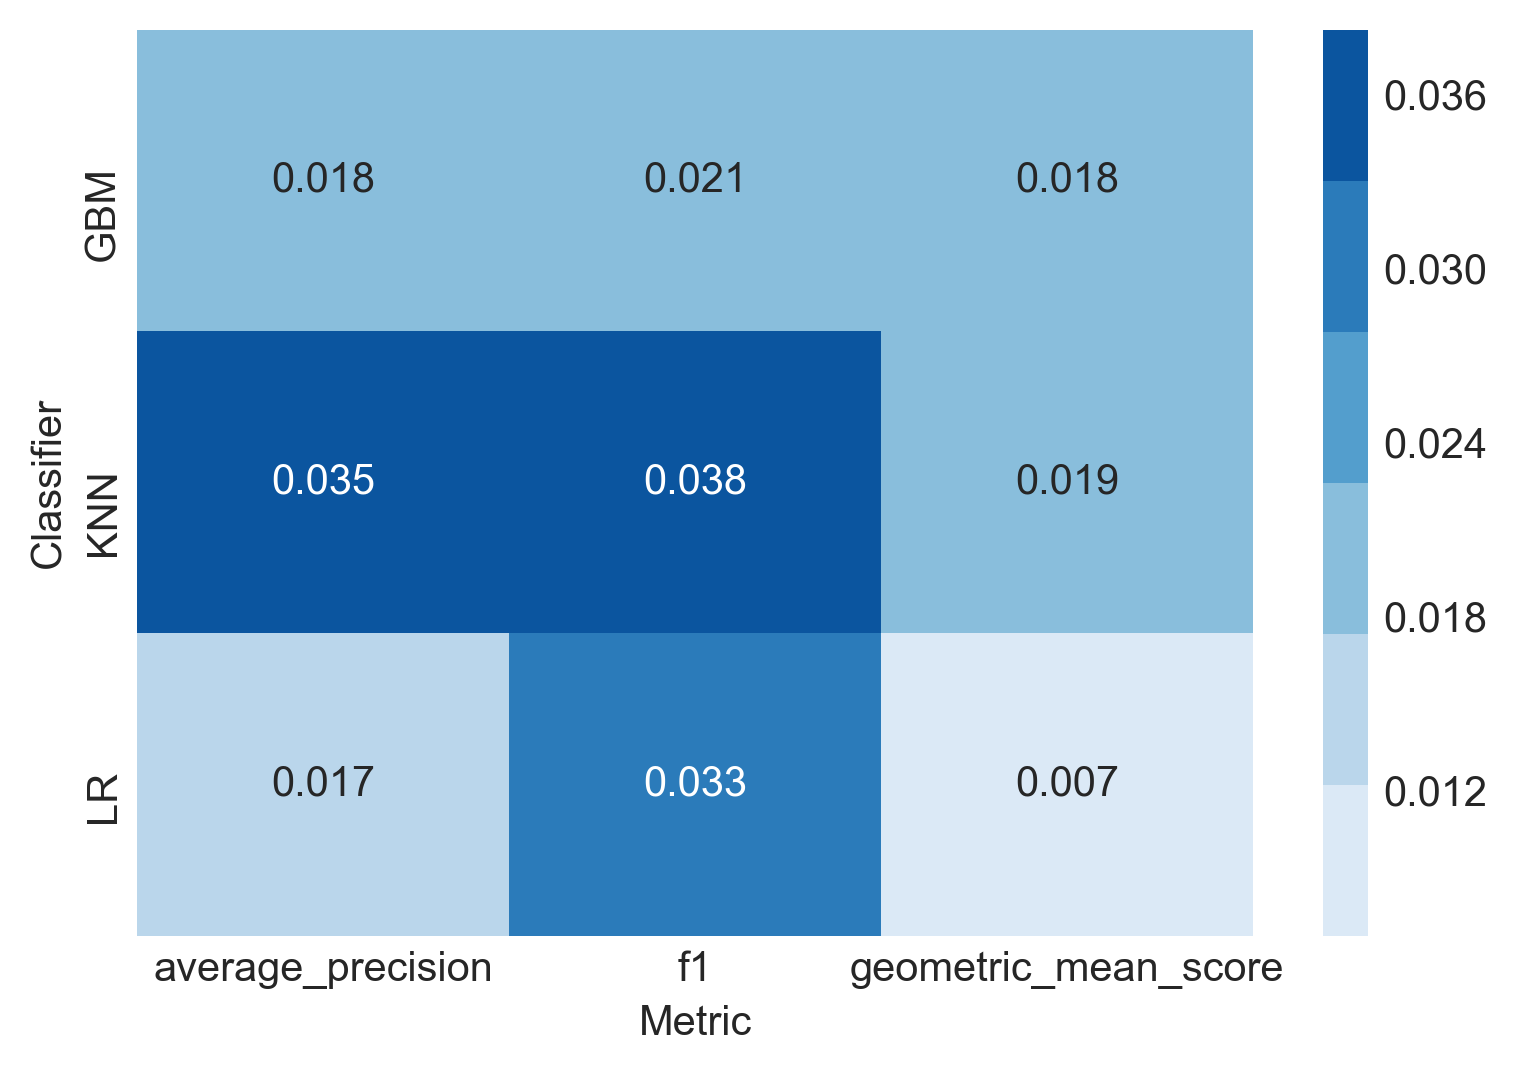
\includegraphics[width=1\linewidth]{../analysis/gains-versus-smote-avg.png}
		\captionof{figure}{Mean score improvement of the proposed method versus \acs{SMOTE} across datasets}
		\label{fig:avg_gains}
	\end{minipage}%
	\hfill
	\begin{minipage}{.48\textwidth}
		\centering
		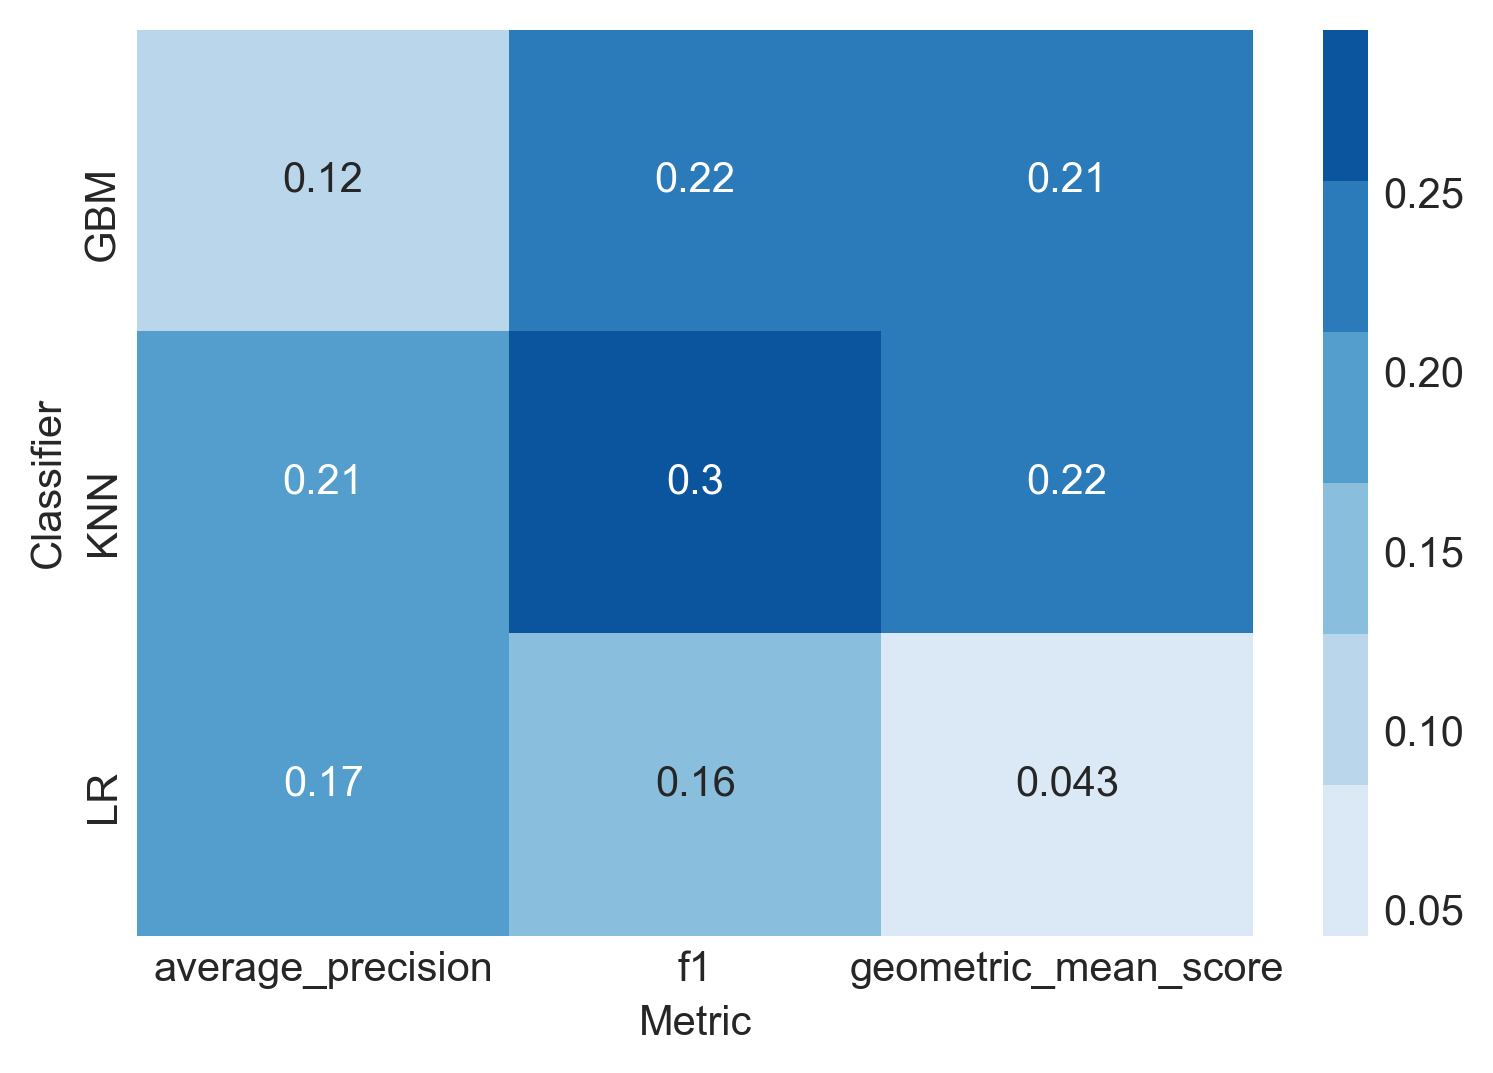
\includegraphics[width=1\linewidth]{../analysis/gains-versus-smote-max.png}
		\captionof{figure}{Maximum score improvement of the proposed method versus \acs{SMOTE}}
		\label{fig:max_gains}
	\end{minipage}
\end{figure}

The \ac{KNN} classifier appears to profit most from the application of k-means
\ac{SMOTE}, where maximum score improvements of more than 0.2 are observed
across all metrics. The biggest mean score improvements are also achieved using
\ac{KNN}, with average gains ranging from 0.019 to 0.035. It can further be
observed that all classifiers benefit from the suggested oversampling procedure.
With only one exception, maximum score improvements of more than 0.1 are found
for all classifiers and metrics.

Taking a closer look at one of the combinations of classifier and metric which,
on average, benefit most from the application of the proposed method,
\cref{fig:comparison} shows the \ac{AUPRC} achieved per dataset by each of the
two oversamplers in conjunction with the \ac{KNN} classifier. Although absolute
scores and score differences between the two methods are dependent on the choice
of metric and classifier, the general trend shown in the figure is observed for
all other metrics and classifiers, which are omitted for clarity.

\begin{figure}[ht]
	\centering
	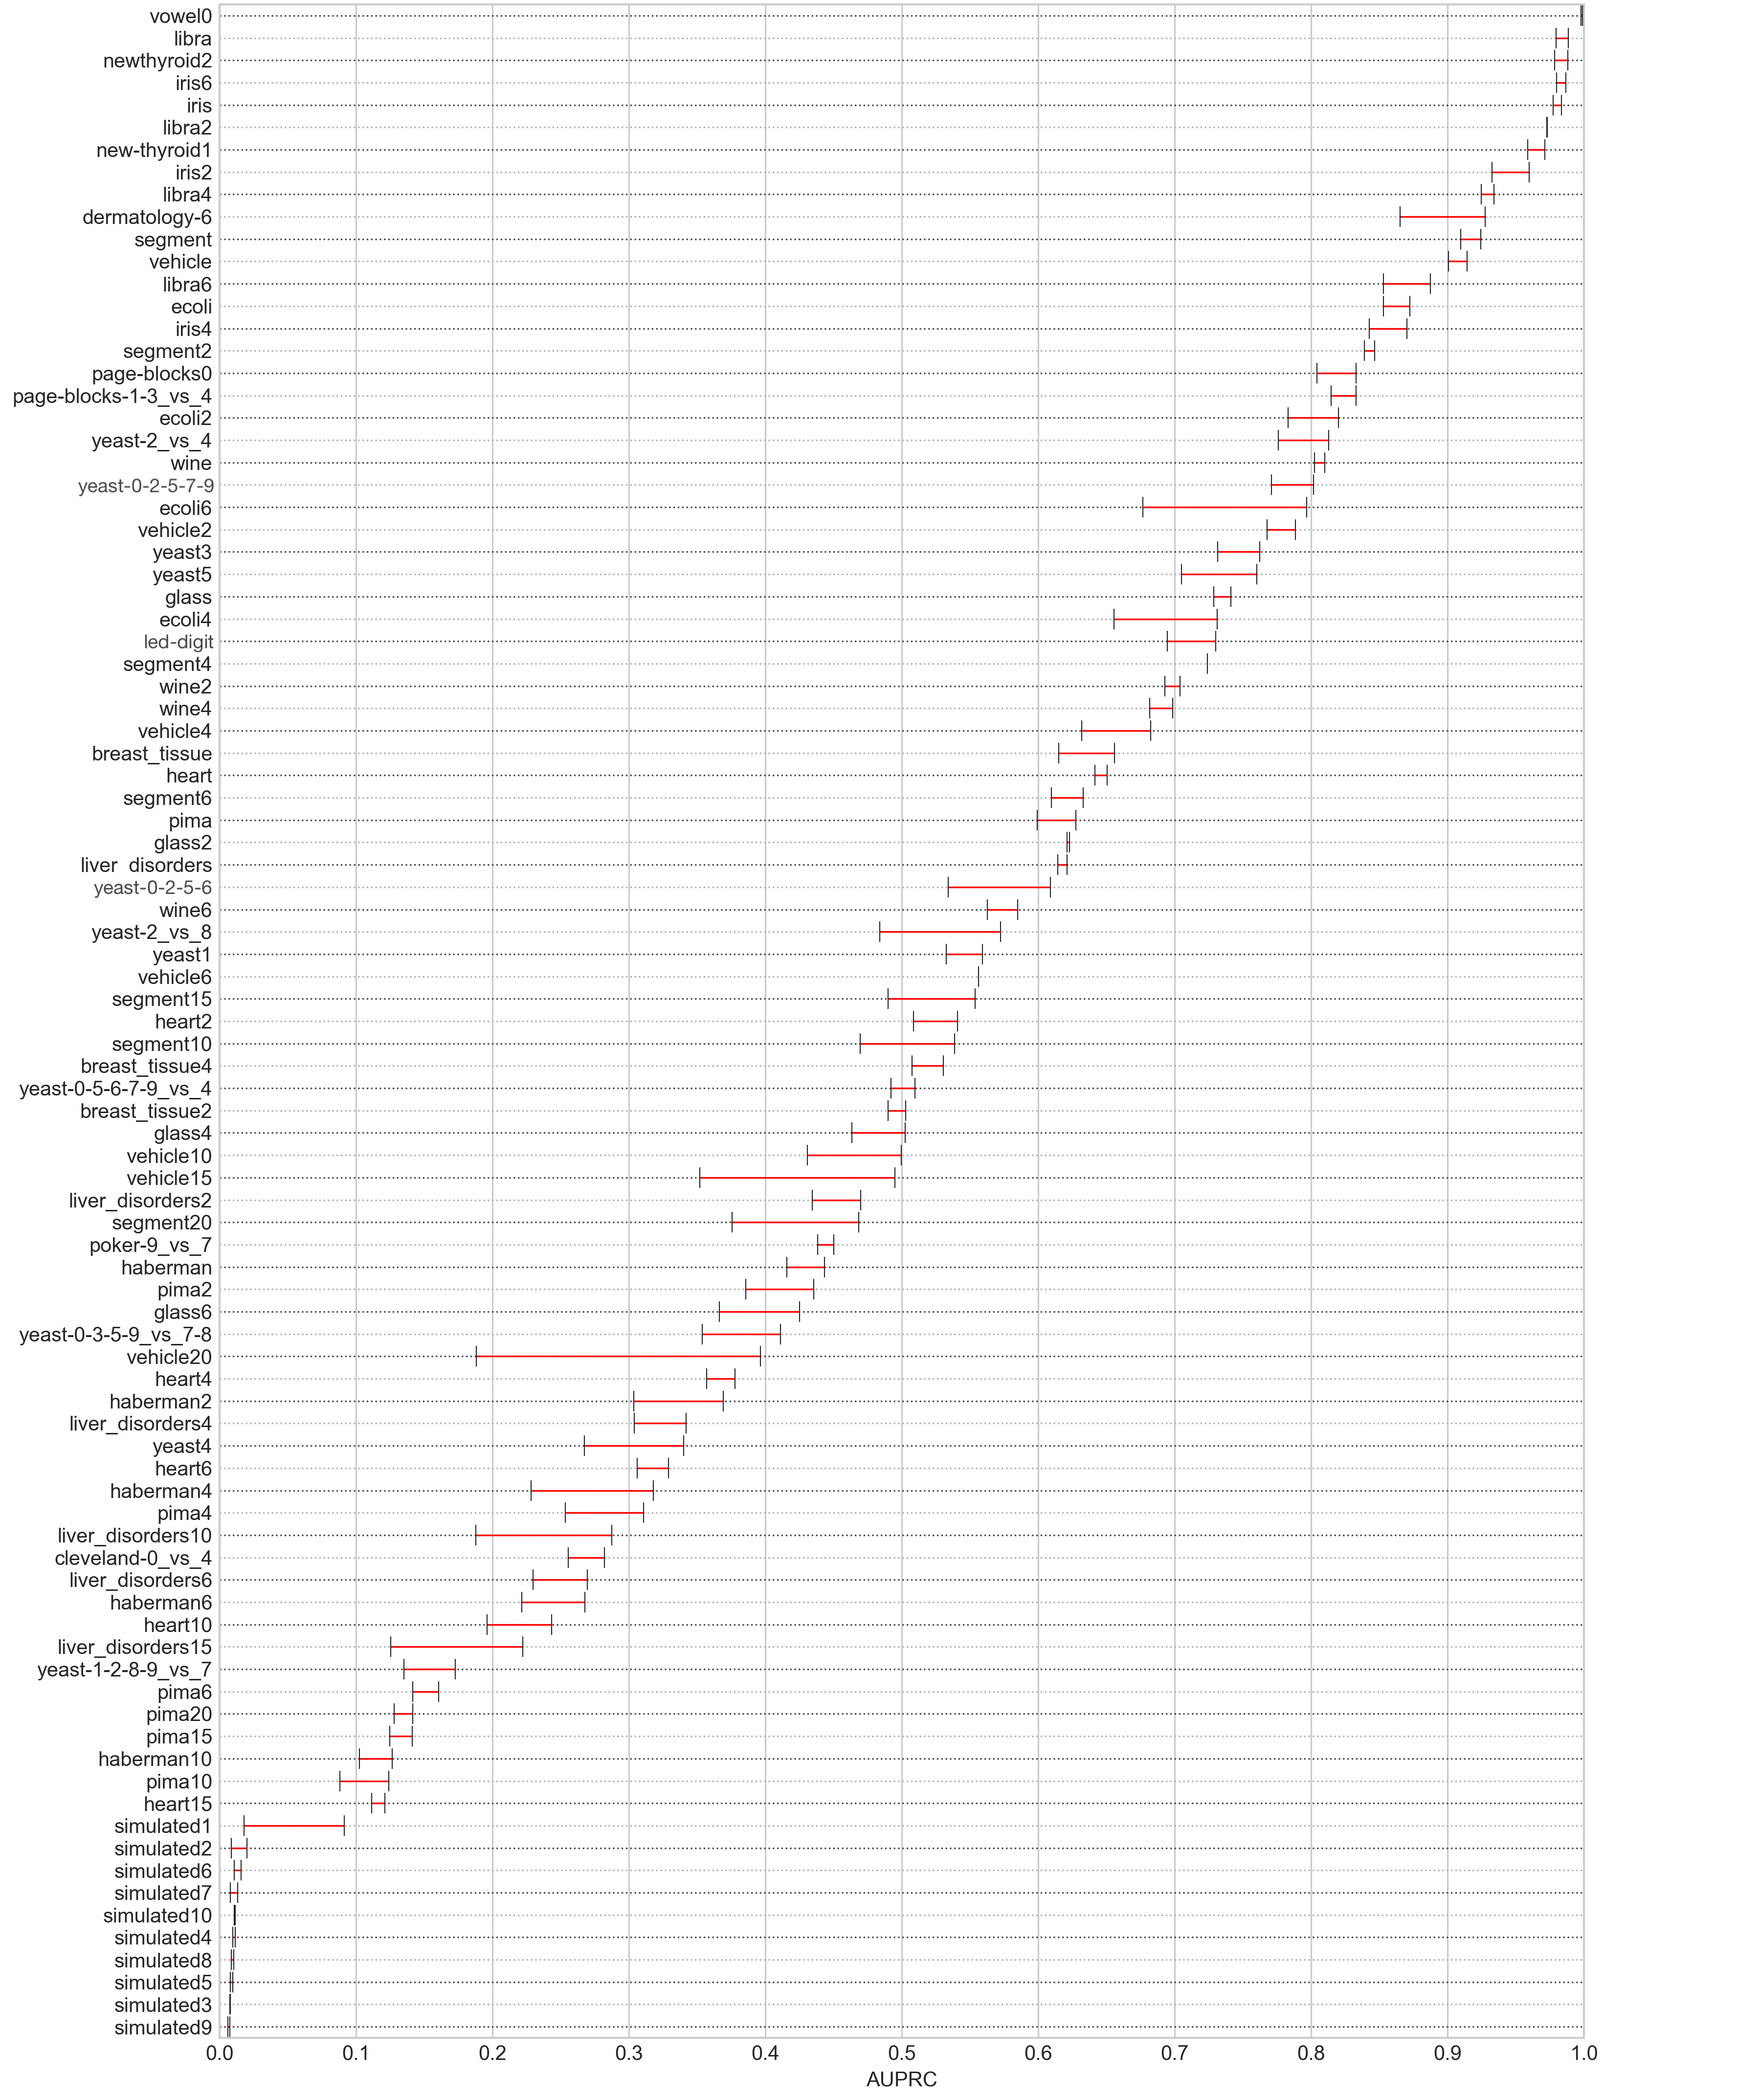
\includegraphics[width=0.87\textwidth]{../analysis/comparison.png}
	\caption[Performance of \acs{KNN} classifier trained on data oversampled with \acs{SMOTE} (left) 
	and k-means \acs{SMOTE} (right)]
	{Performance of \acs{KNN} classifier trained on different datasets
	oversampled with \acs{SMOTE} (left) and k-means \acs{SMOTE} (right) ordered
	by \acs{AUPRC}}
	\label{fig:comparison}
\end{figure}

In the large majority of cases, k-means \ac{SMOTE} outperforms \ac{SMOTE},
proving the relevance of the clustering procedure. Only in 6 out of 90 datasets
tested there were no improvements through the use of k-means \ac{SMOTE}. On
average, k-means \ac{SMOTE} achieves an \ac{AUPRC} improvement of 0.035. The
biggest gains of the proposed method appear to be occurring in the score range
of 0.2 to 0.8. The biggest gain of approximately 0.2 is achieved for dataset
``vehicle20''. The score difference among oversamplers is smaller at the extreme
ends of the scale. For nine of the simulated datasets, \ac{KNN} attains a score
very close to zero independently of the choice of the oversampler. Similarly,
for the datasets where an exceptionally high \ac{AUPRC} is attained (``vowel0'',
``libra'', ``newthyroid2'', ``iris6'', ``iris'', ``libra2''), gains of k-means
\ac{SMOTE} are less than 0.03.

As described in \cref{sec:related-work,,sec:proposed-method}, a core goal of the
applied clustering approach is to avoid the generation of noise, which
\ac{SMOTE} is predisposed to amplify. Since minority samples generated in
majority class regions may contribute to an increase in false positives, the
false positive count can be regarded as an indicator of the level of noise
generation. As a basis to analyze whether the proposed oversampler successfully
reduces the generation of noise, \cref{fig:false_positives_reduction} visualizes
the number of false positives after the application of k-means \ac{SMOTE} as a
percentage of the number of false positives observed using \ac{SMOTE}. The false
positive counts used in the chart are averages across experiment repetitions,
choosing the hyperparameter configuration which attains the lowest number for
each technique.

\begin{figure}[ht]
	\centering
	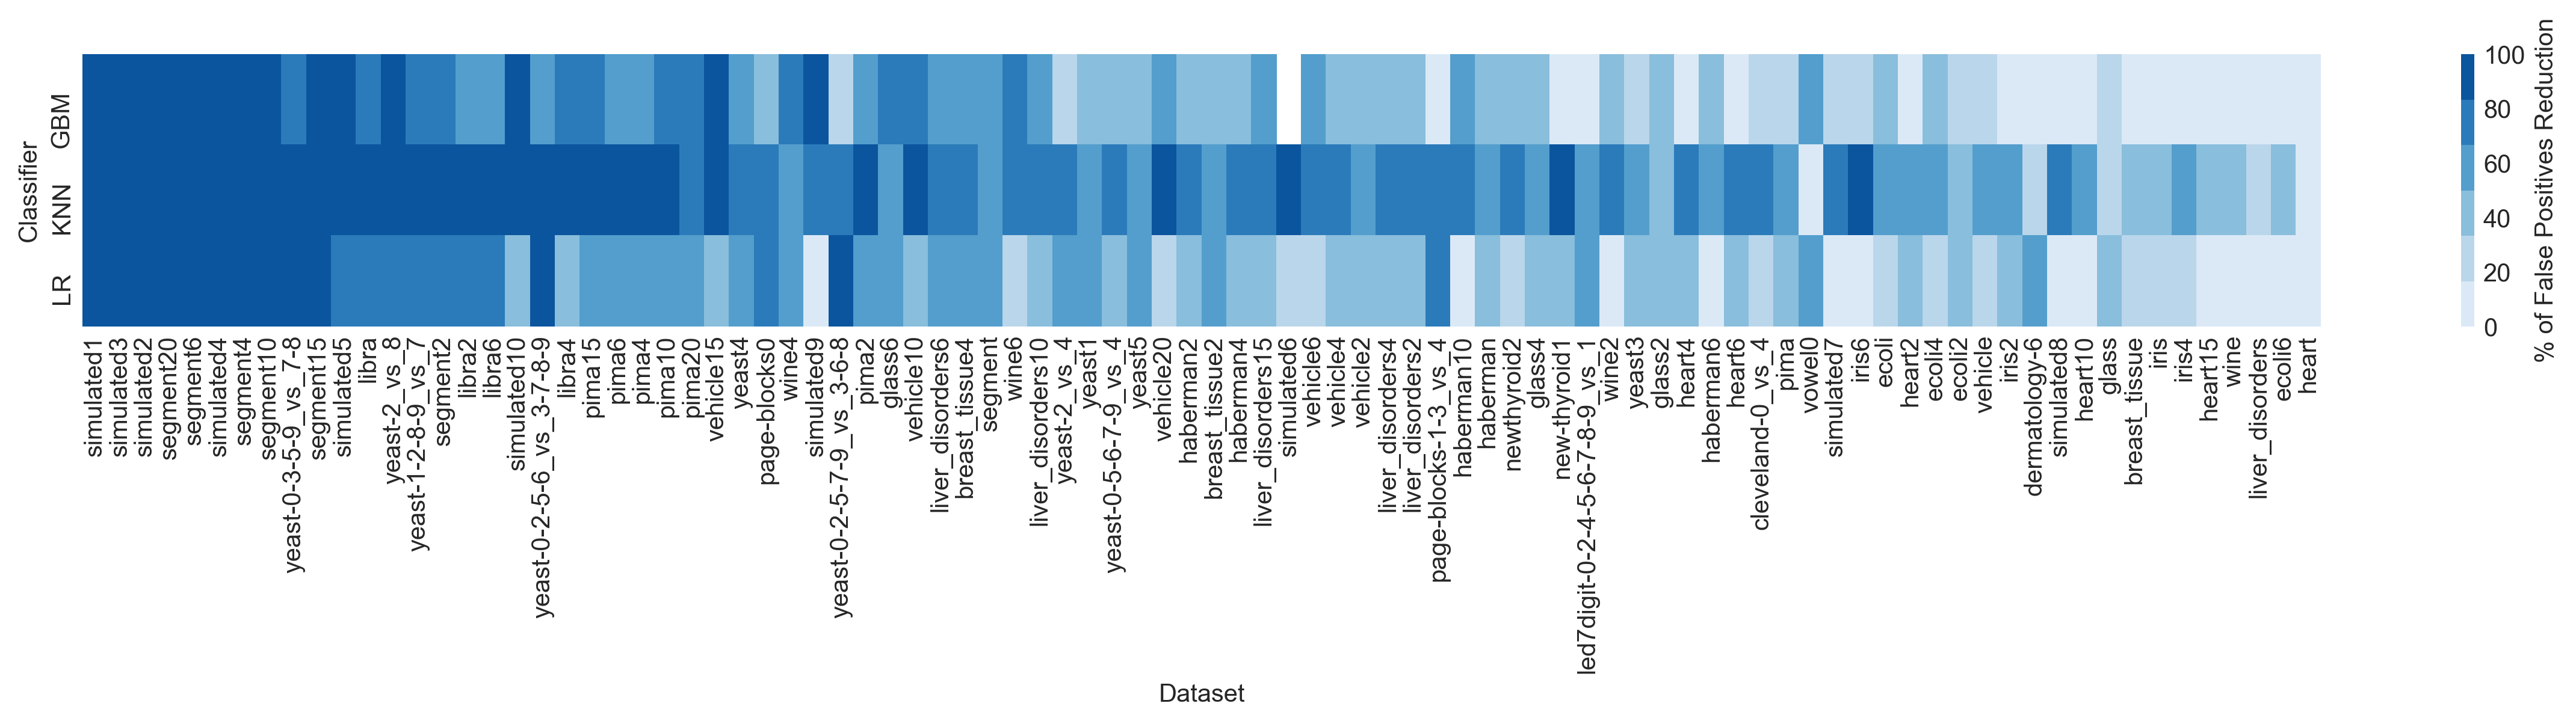
\includegraphics[width=\textwidth]{../analysis/false-positives-reduction-vs-smote.png}
	\caption[Relative reduction of false positives compared to \acs{SMOTE}]
	{Relative reduction of false positives compared to \acs{SMOTE} ordered from
	highest to lowest average reduction. A high percentage indicates that the
	proposed method generates fewer minority samples in majority regions than
	the baseline method.}
	\label{fig:false_positives_reduction}
\end{figure}

The figure illustrates that k-means \ac{SMOTE} is able to reduce the number of
false positives compared to \ac{SMOTE} in every dataset and independently of the
classifier (with a single exception). In many cases, k-means \ac{SMOTE}
eliminates more than 90\% of false positives in comparison to the baseline
method. On average, a 55\% reduction of false positives compared to \ac{SMOTE}
is found, the biggest improvements being attained by the \ac{KNN} classifier.
Among the datasets where over 80\% of false positives could be avoided are the
artificial datasets as well as variations of the datasets ``segment'', ``yeast''
and ``libra''.

Using two-dimensional toy datasets, it is possible to illustrate how k-means
\ac{SMOTE} may improve the results attained by plain \ac{SMOTE}.
\Cref{fig:toy-a,fig:toy-b,fig:toy-c,fig:toy-circles,fig:toy-moons} show the
result of applying both methods to simple binary datasets with two to three
distinct, albeit slightly noisy, clusters. For all datasets, we observe that
\ac{SMOTE} generates minority samples within majority clusters or directly on
the class border. In contrast, the proposed method avoids data generation
outside of minority clusters. Particularly \cref{fig:toy-circles,fig:toy-moons}
exemplify how overlapping class areas are not subject to data generation as they
are deemed unsafe. Illustrating the suggested technique's ability to rebalance
within classes, \cref{fig:toy-b} shows that \ac{SMOTE} is inclined to generate
most samples in the already dense cluster on the bottom right. In contrast,
k-means \ac{SMOTE} recognizes that the cluster on the top left is sparsely
populated and focuses data generation there. Overall, the toy datasets
demonstrate that the proposed method is apt to achieve balance between and
within classes, while at the same time avoiding noise generation.

\begin{figure}[ht]
	\centering
	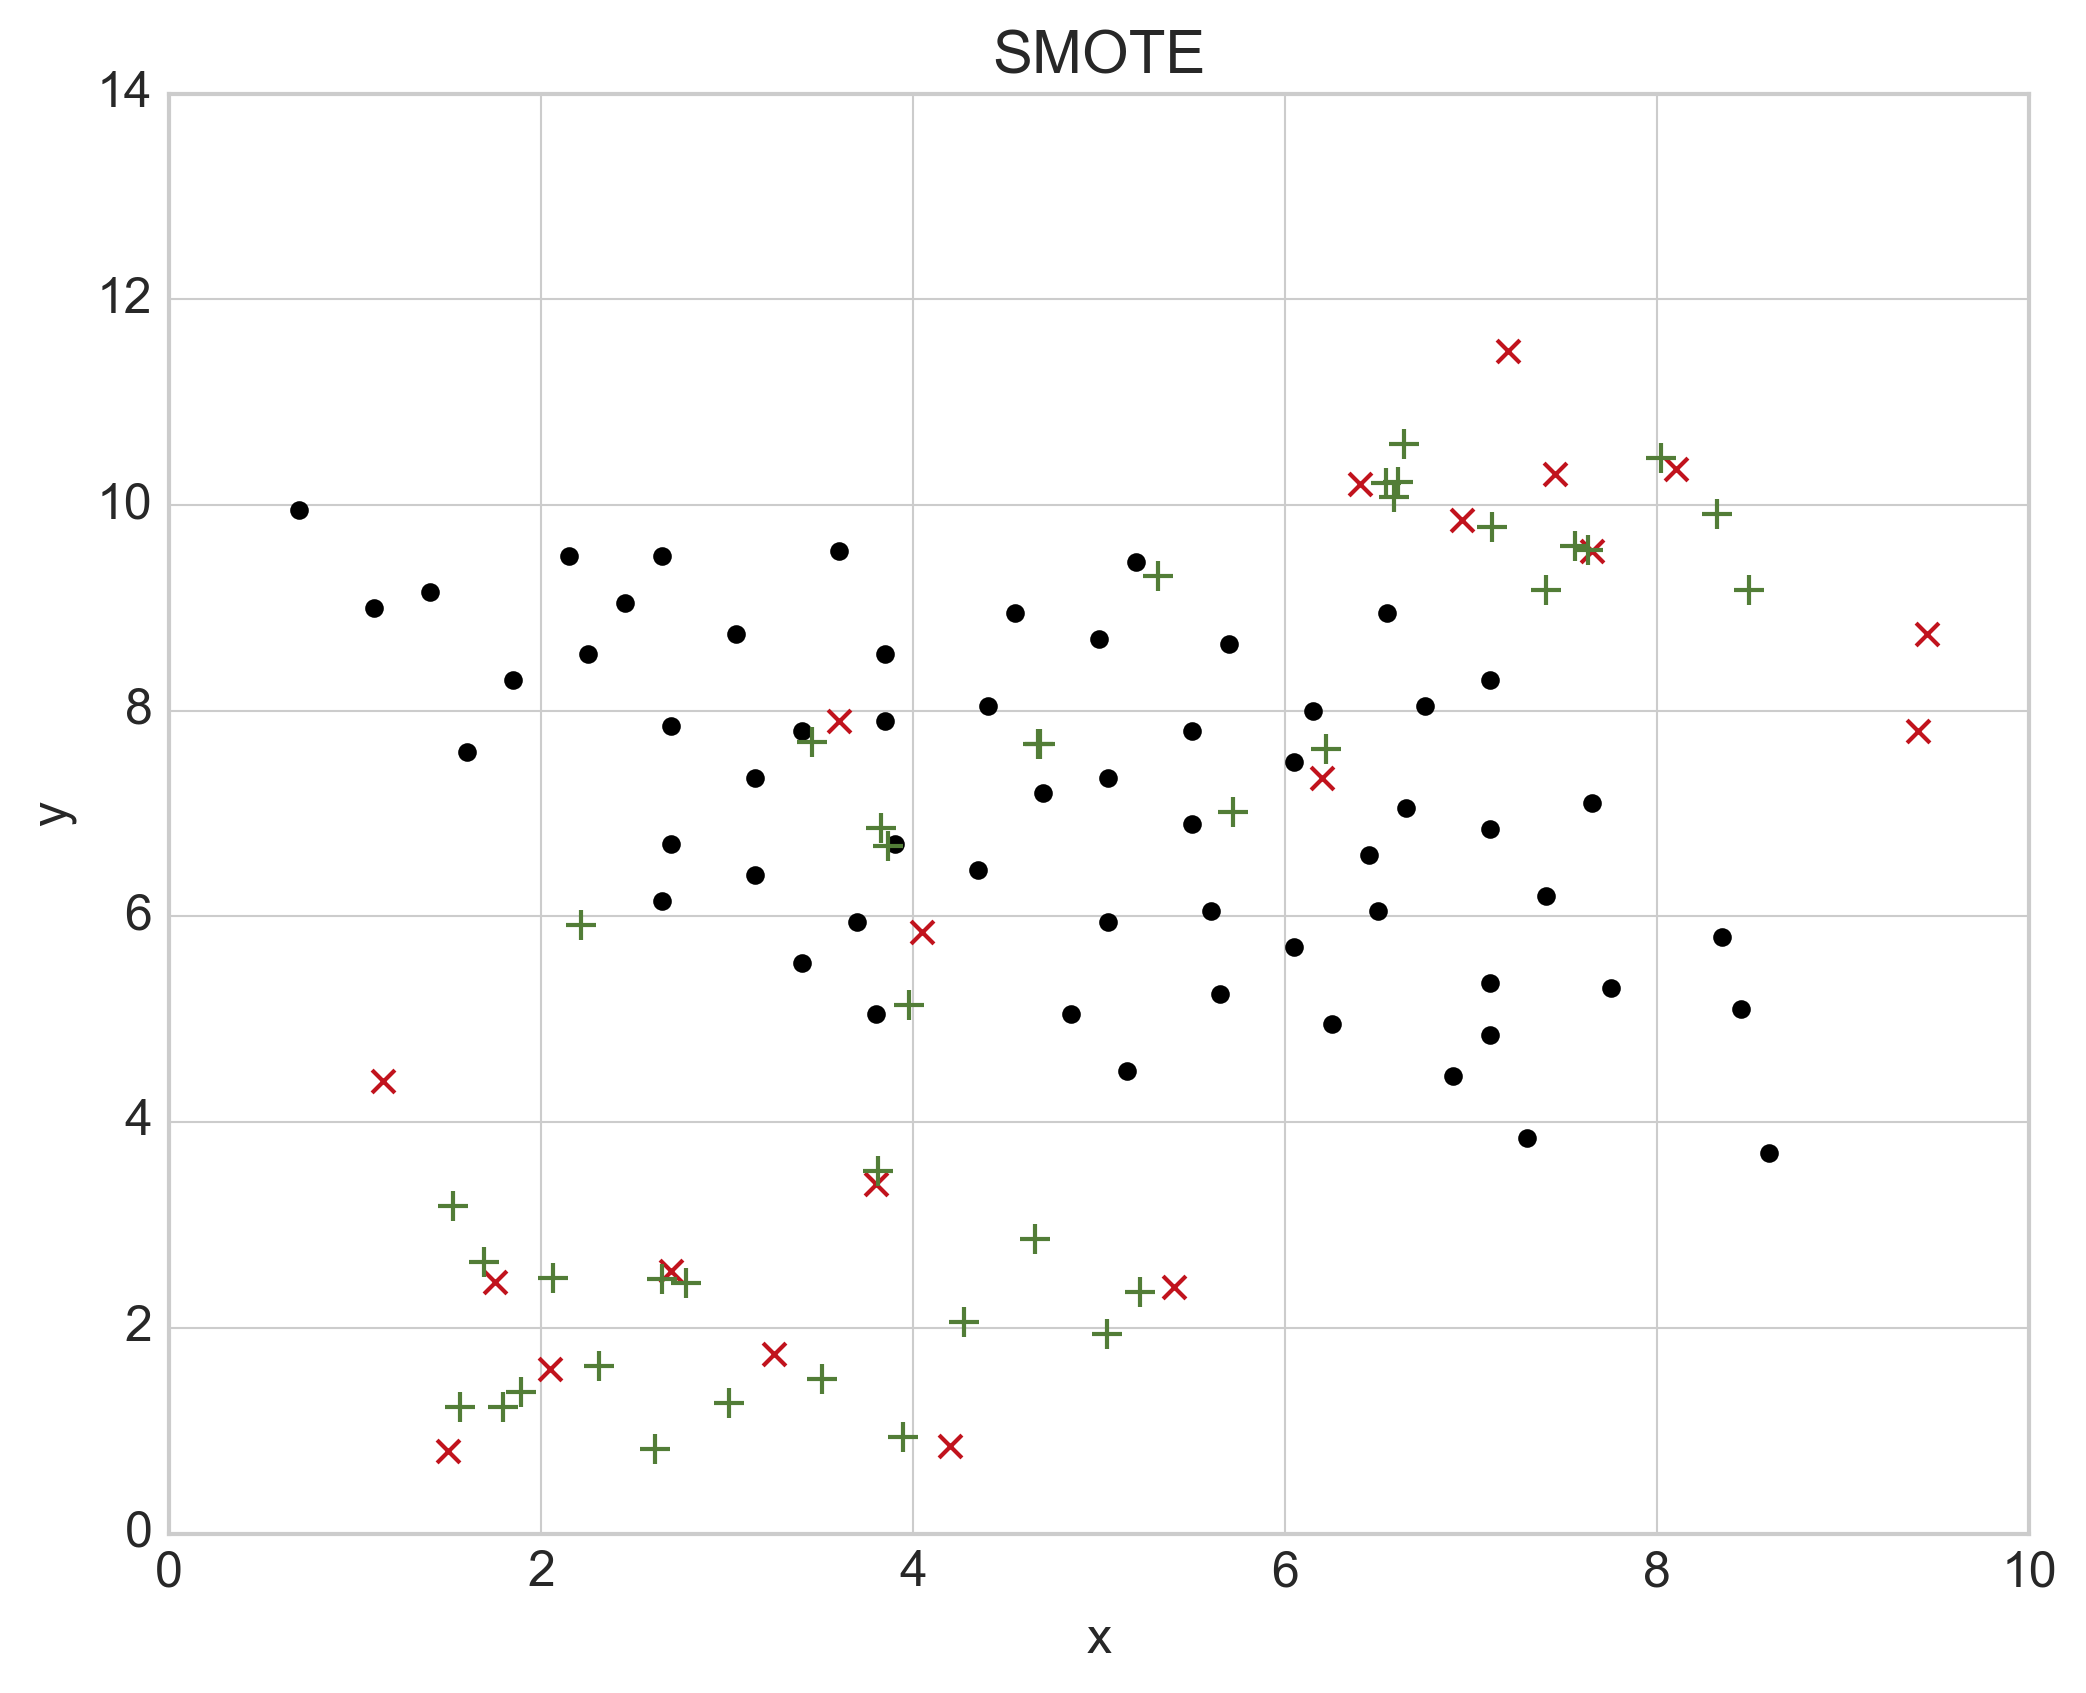
\includegraphics[width=.48\linewidth]{../analysis/A_SMOTE.png}
	\hfill
	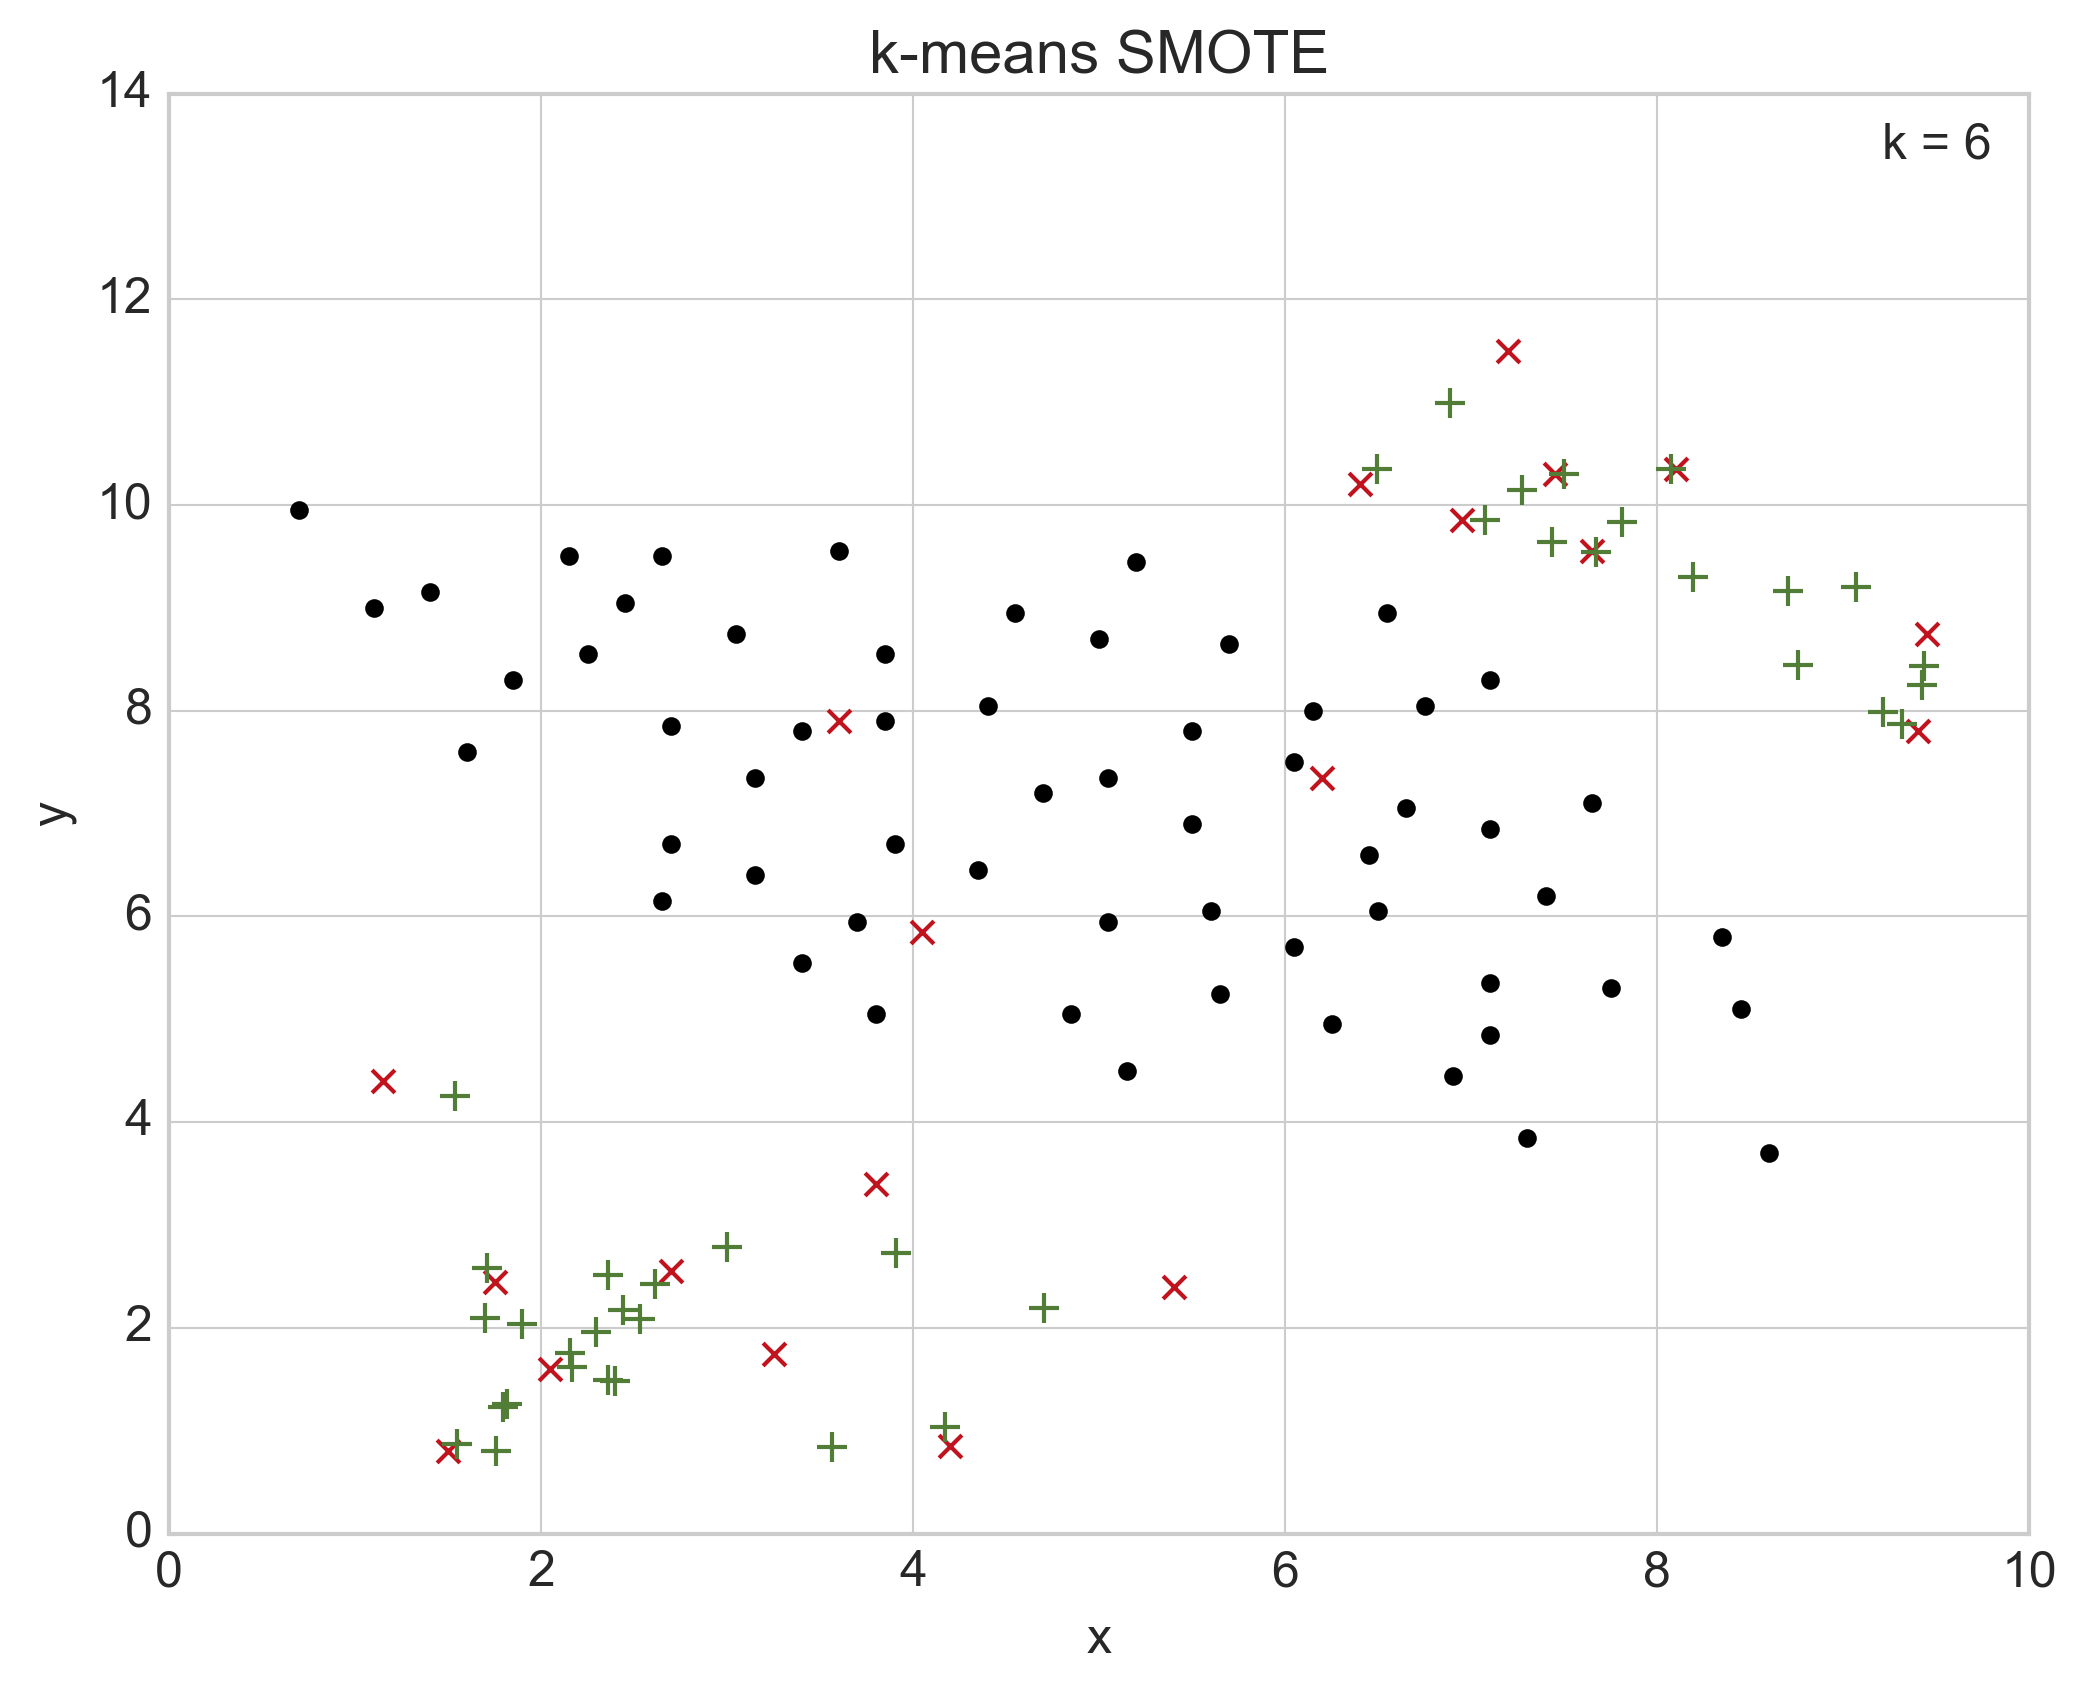
\includegraphics[width=.48\linewidth]{../analysis/A_k-means_SMOTE.png}
	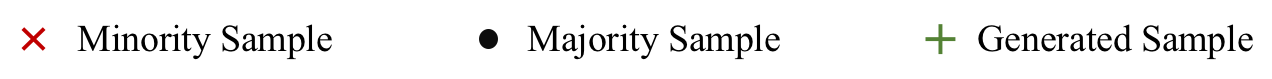
\includegraphics[width=.6\linewidth]{../analysis/legend.png}
	\captionof{figure}[Demonstration of oversampling toy dataset A with \acs{SMOTE} and k-means \acs{SMOTE}]
	{Samples generated through oversampling toy dataset A with \acs{SMOTE} (left) and k-means \acs{SMOTE} (right)}
	\label{fig:toy-a}
 \end{figure}

 \begin{figure}[ht]
	\centering
	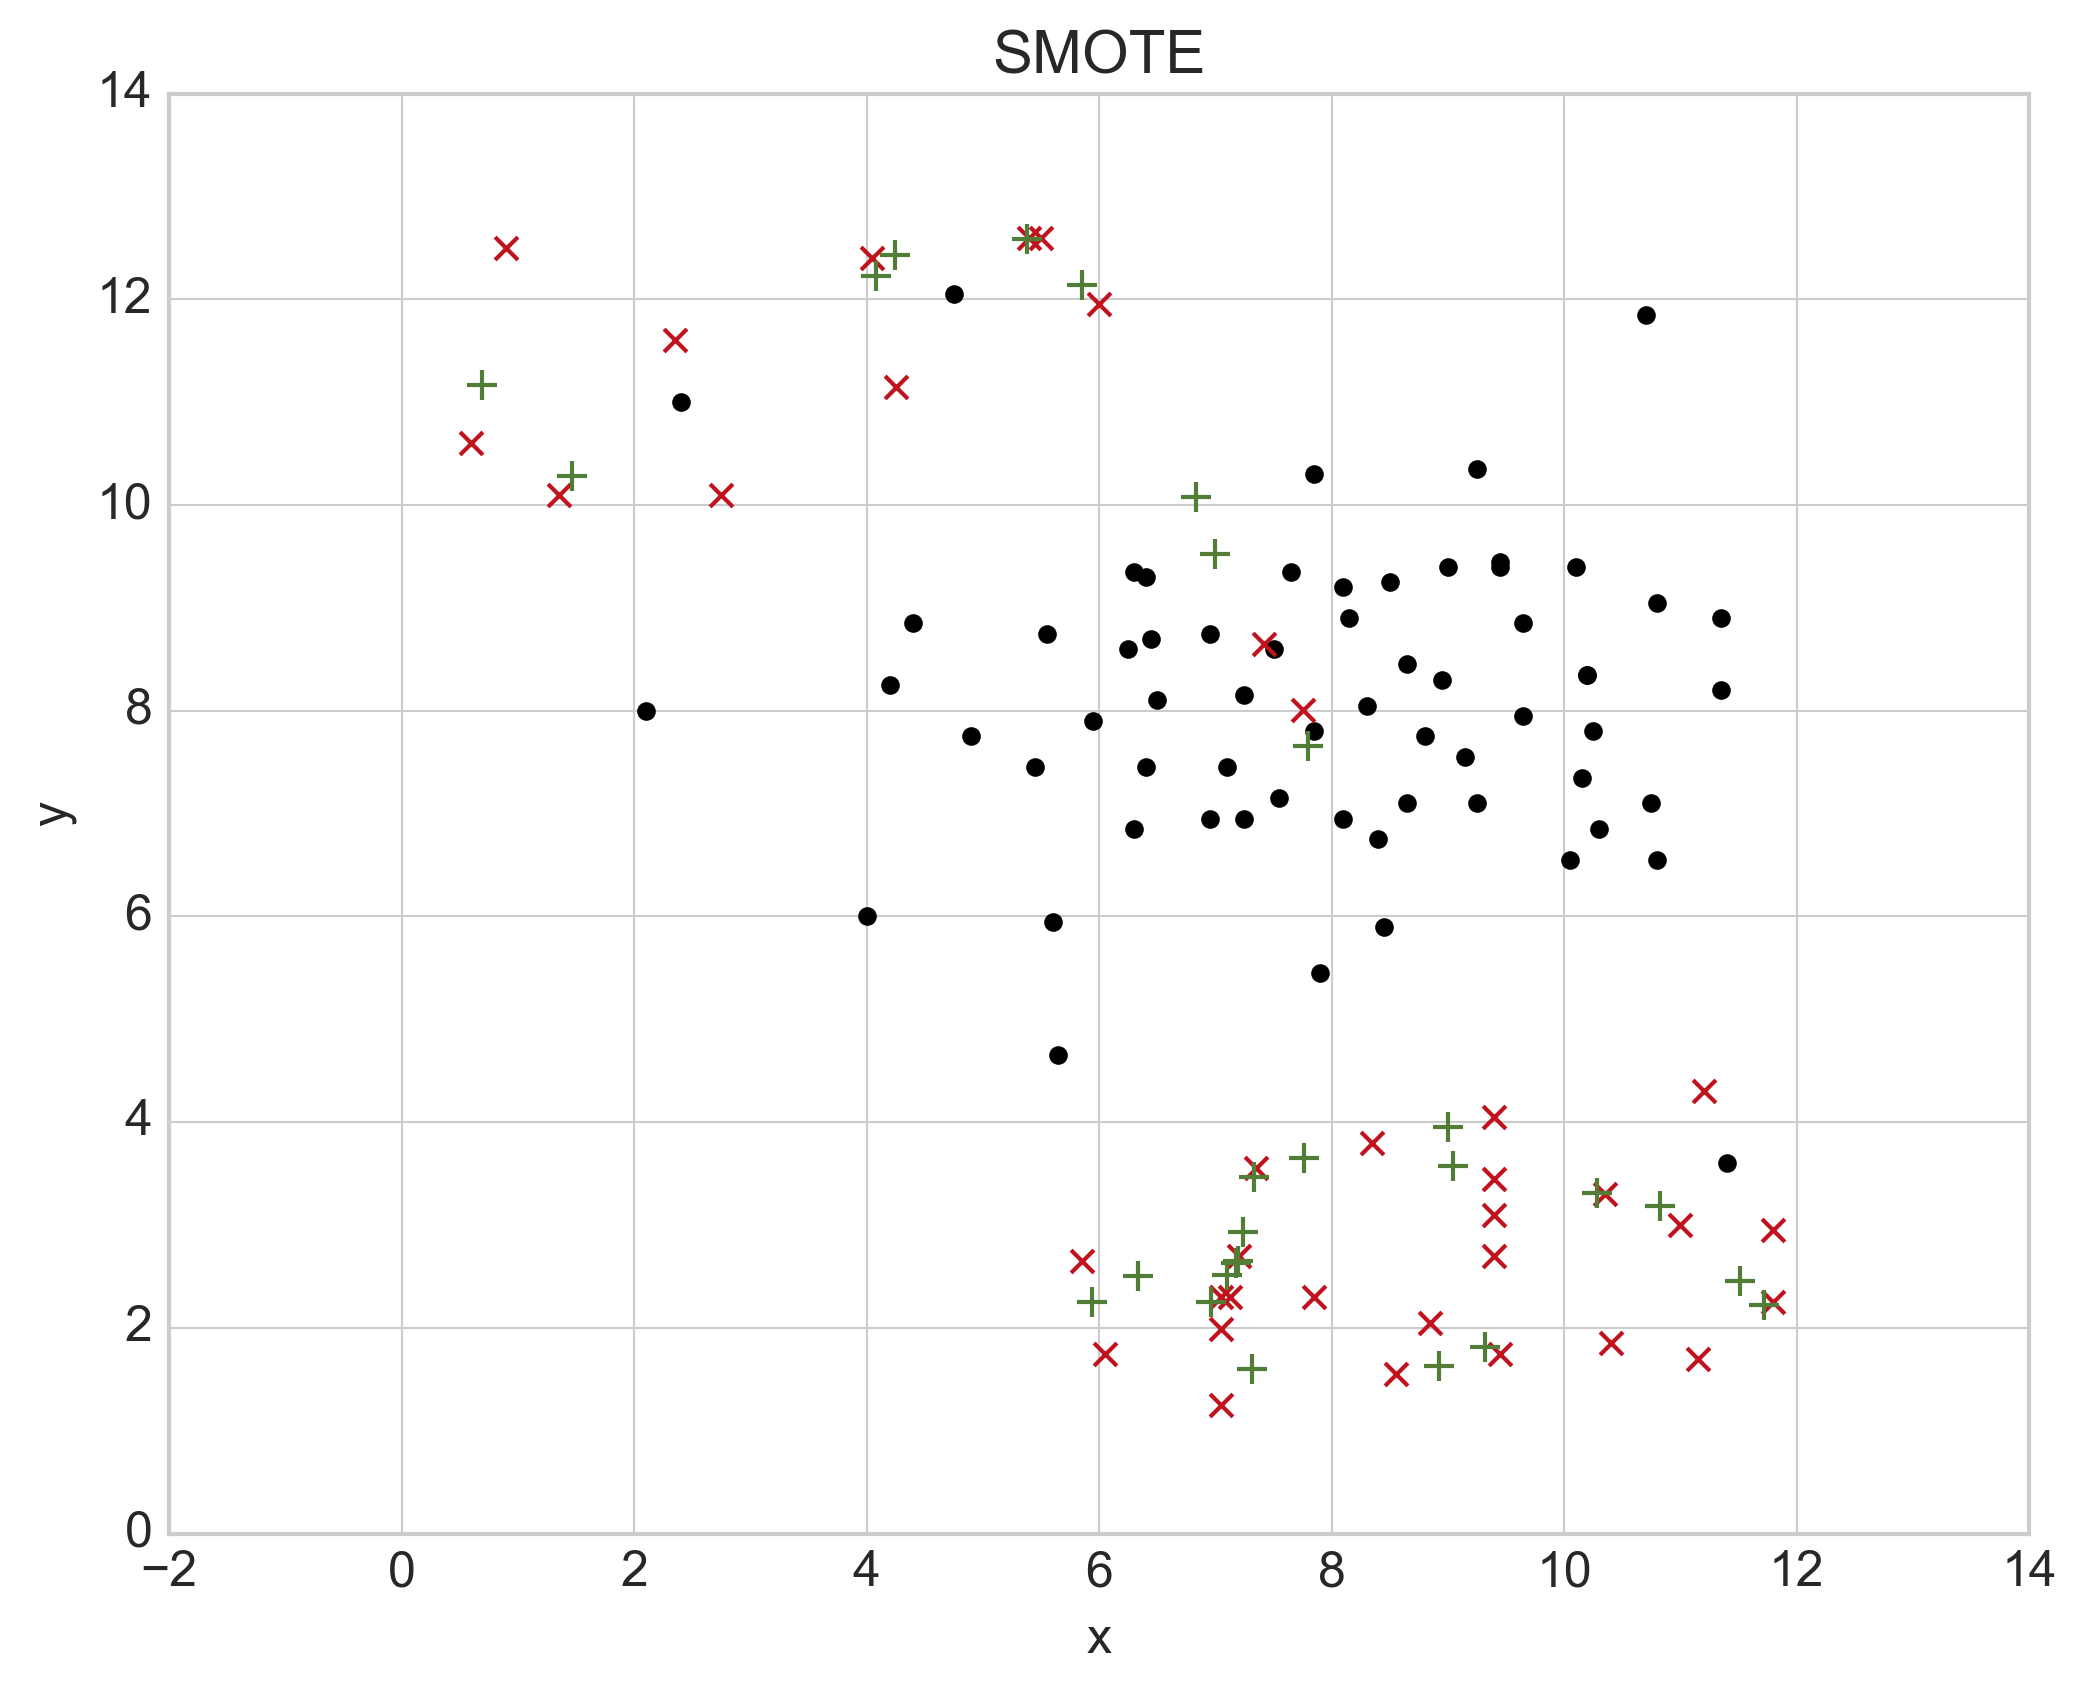
\includegraphics[width=.48\linewidth]{../analysis/B_SMOTE.png}
	\hfill
	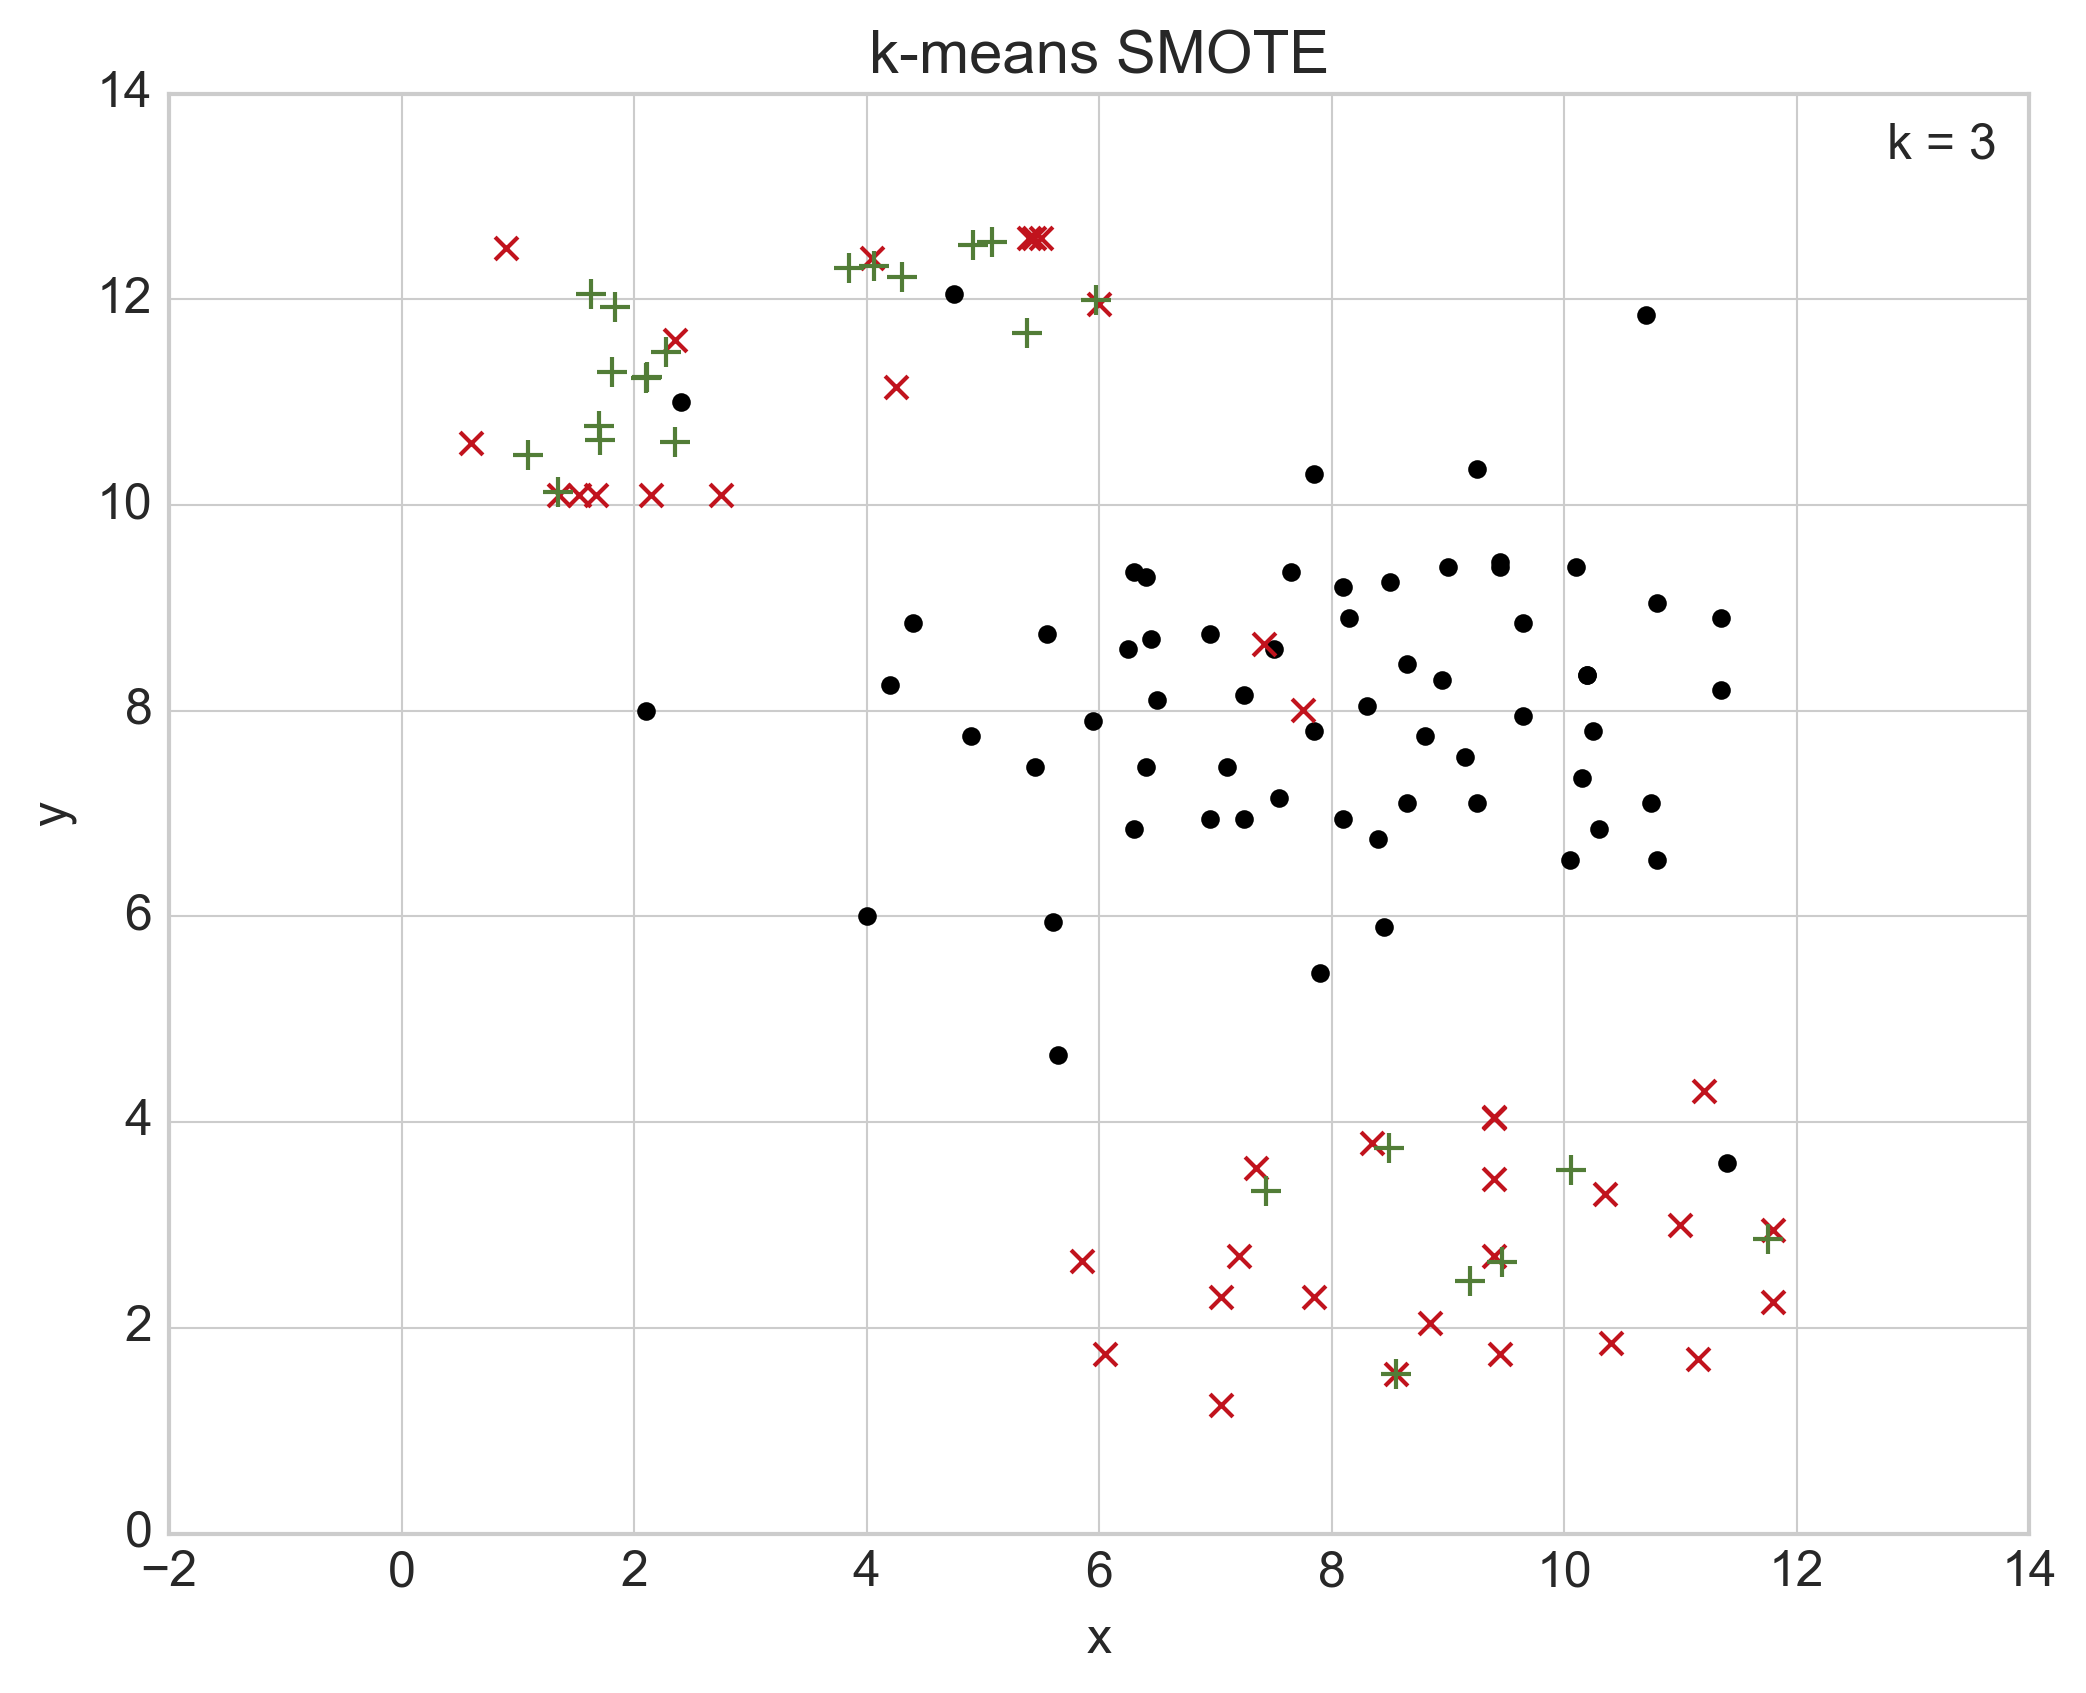
\includegraphics[width=.48\linewidth]{../analysis/B_k-means_SMOTE.png}
	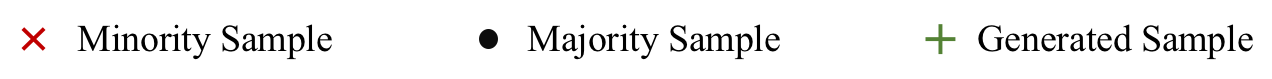
\includegraphics[width=.6\linewidth]{../analysis/legend.png}
	\captionof{figure}{Samples generated through oversampling toy dataset B with \acs{SMOTE} and k-means \acs{SMOTE}}
	\label{fig:toy-b}
 \end{figure}

 \begin{figure}[ht]
	\centering
	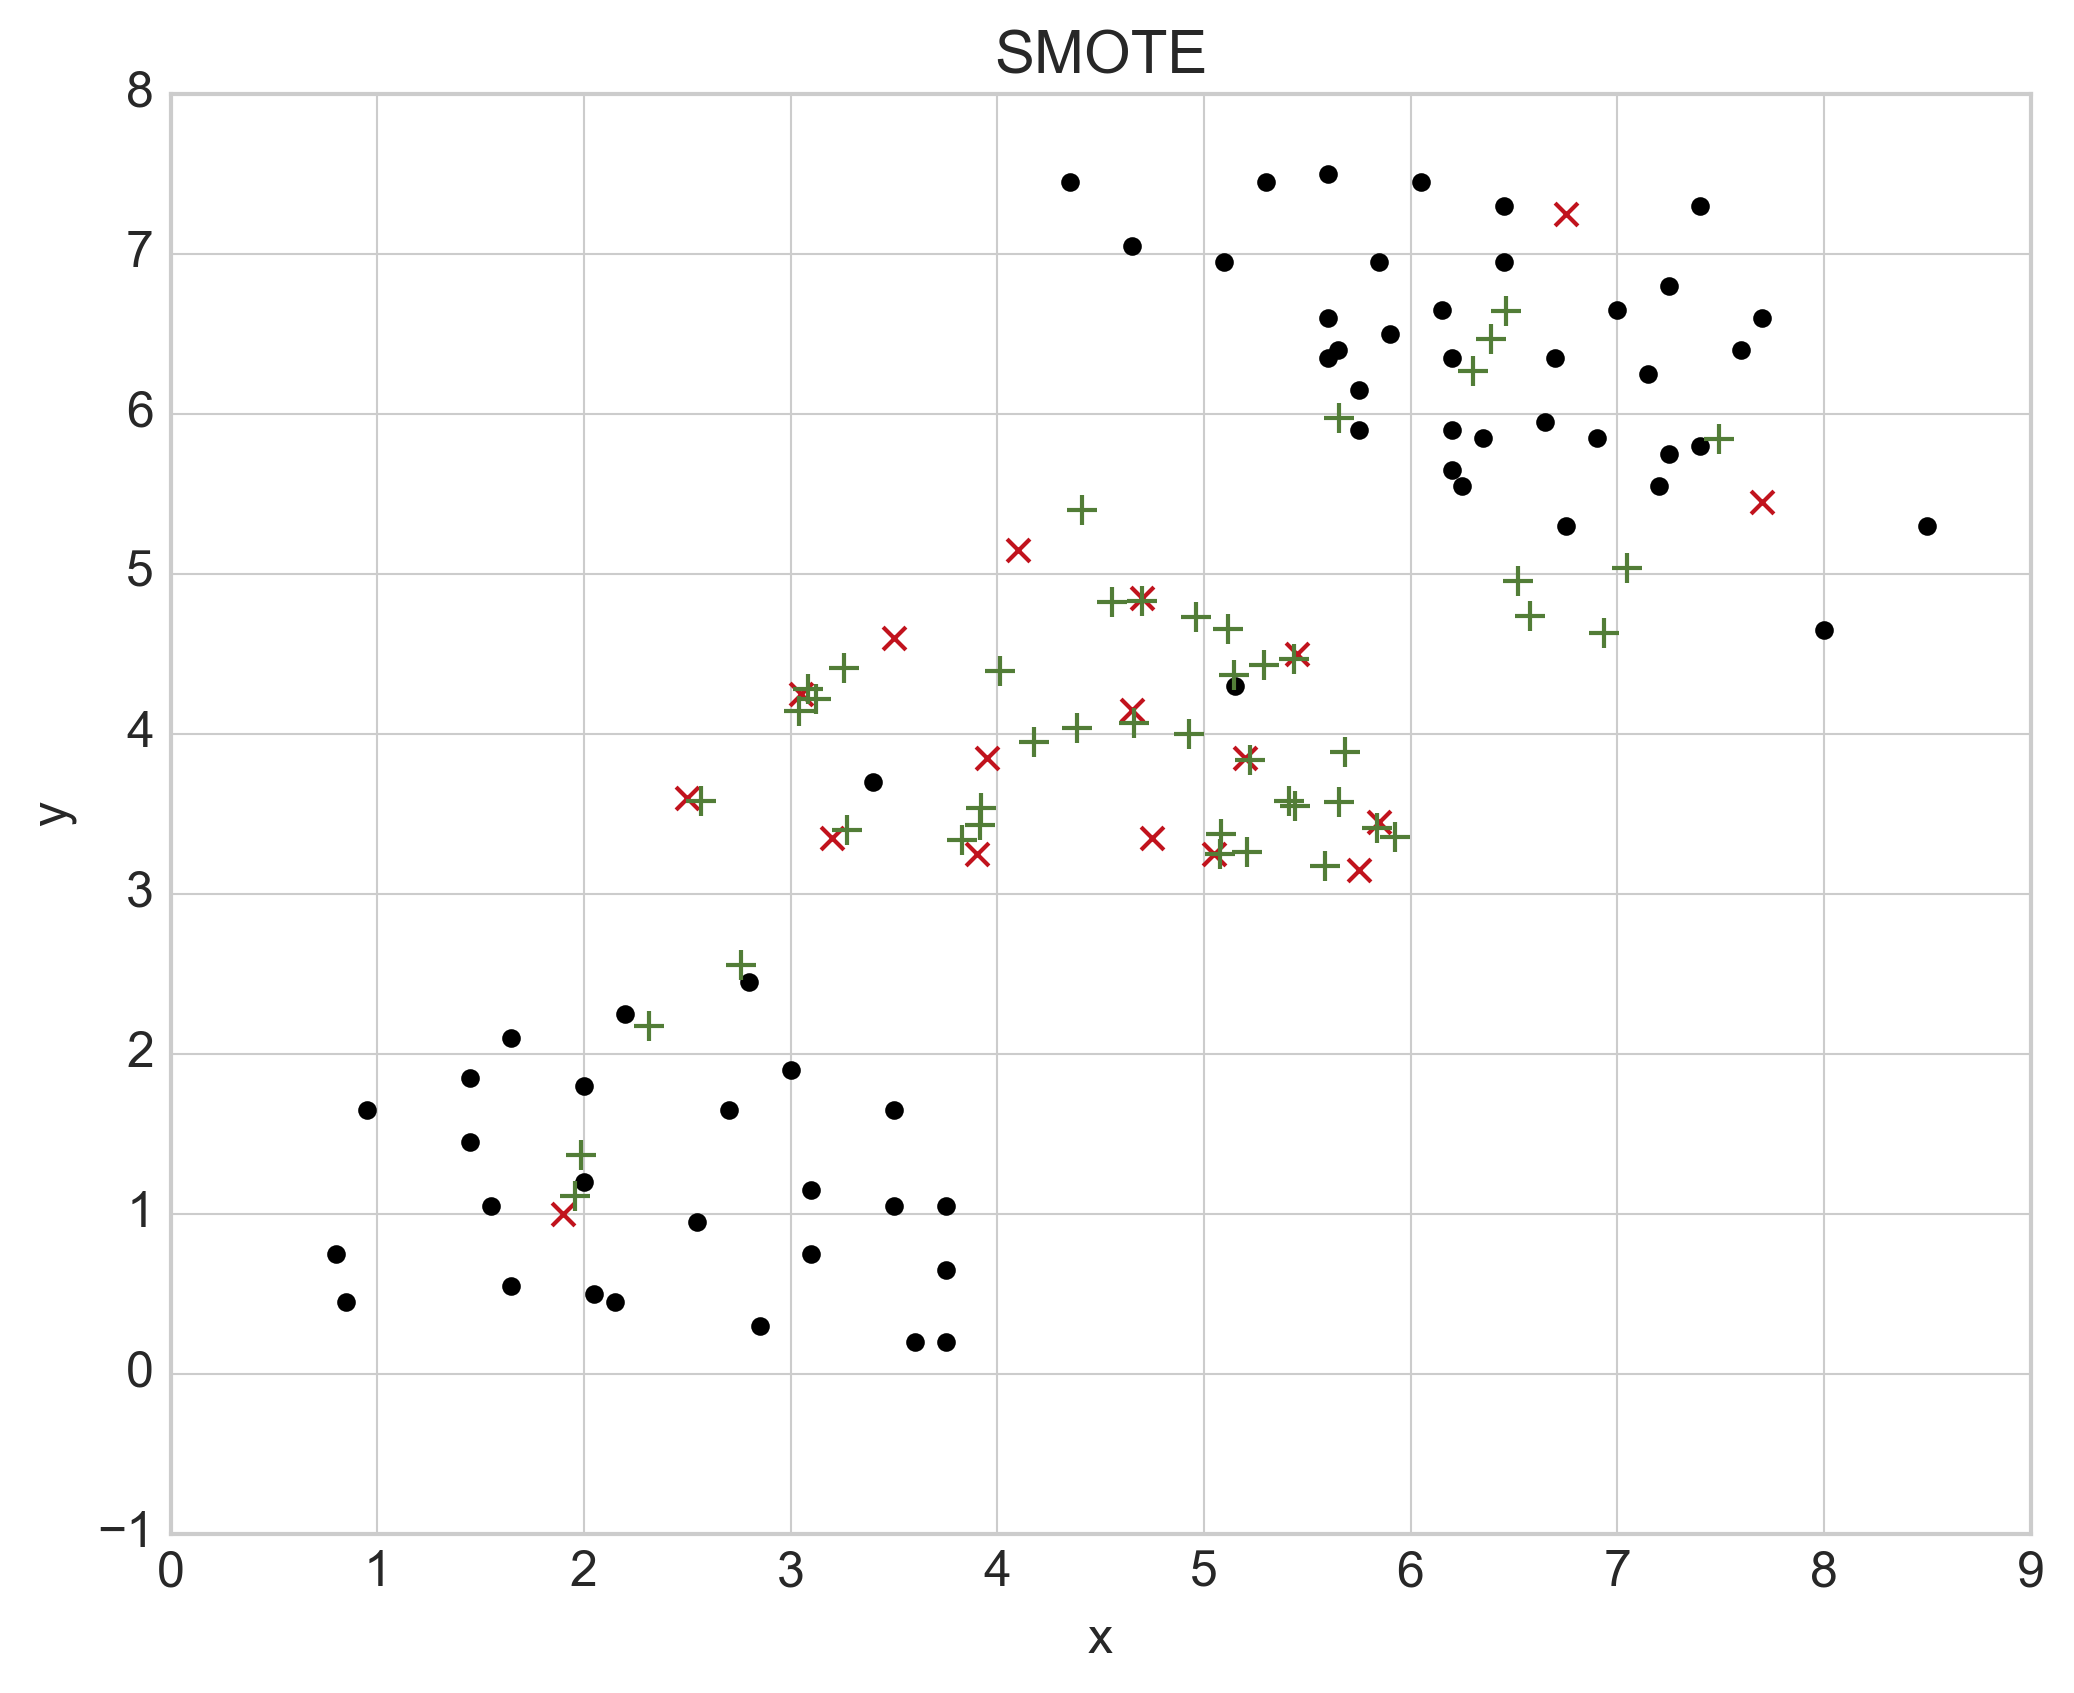
\includegraphics[width=.48\linewidth]{../analysis/C_SMOTE.png}
	\hfill
	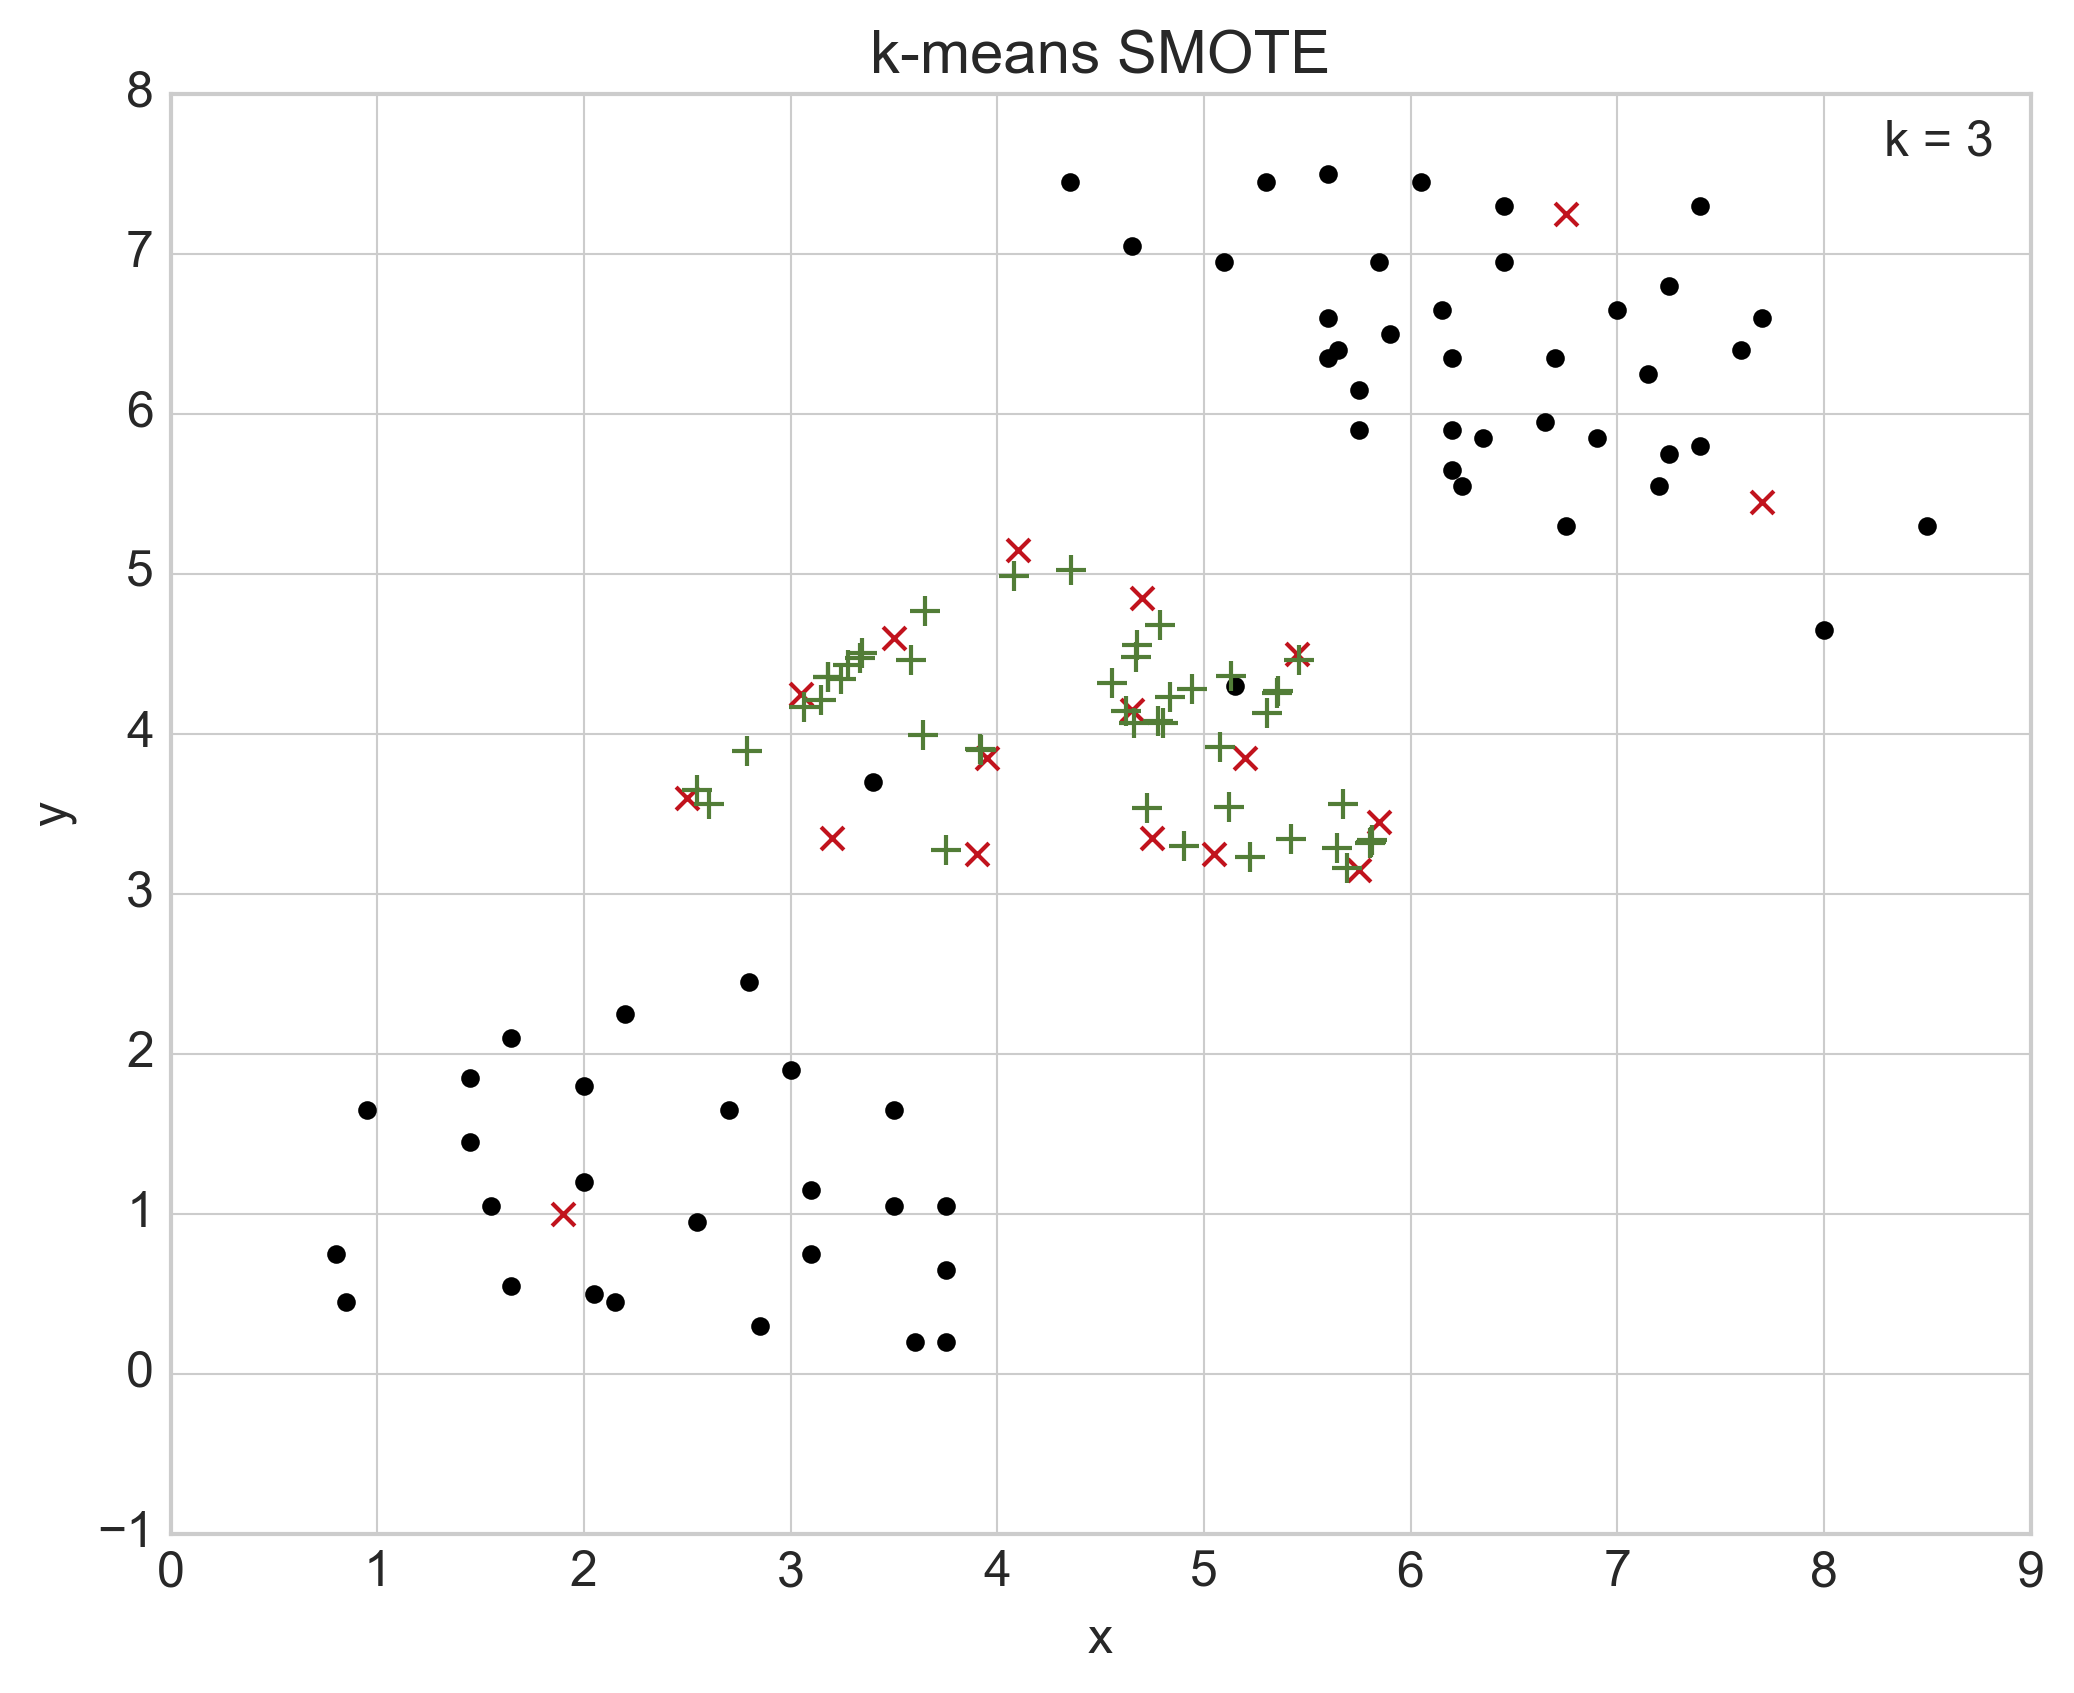
\includegraphics[width=.48\linewidth]{../analysis/C_k-means_SMOTE.png}
	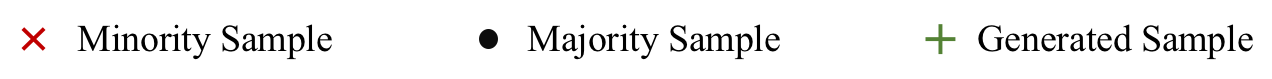
\includegraphics[width=.6\linewidth]{../analysis/legend.png}
	\captionof{figure}{Samples generated through oversampling toy dataset C with \acs{SMOTE} and k-means \acs{SMOTE}}
	\label{fig:toy-c}
 \end{figure}

  \begin{figure}[ht]
	\centering
	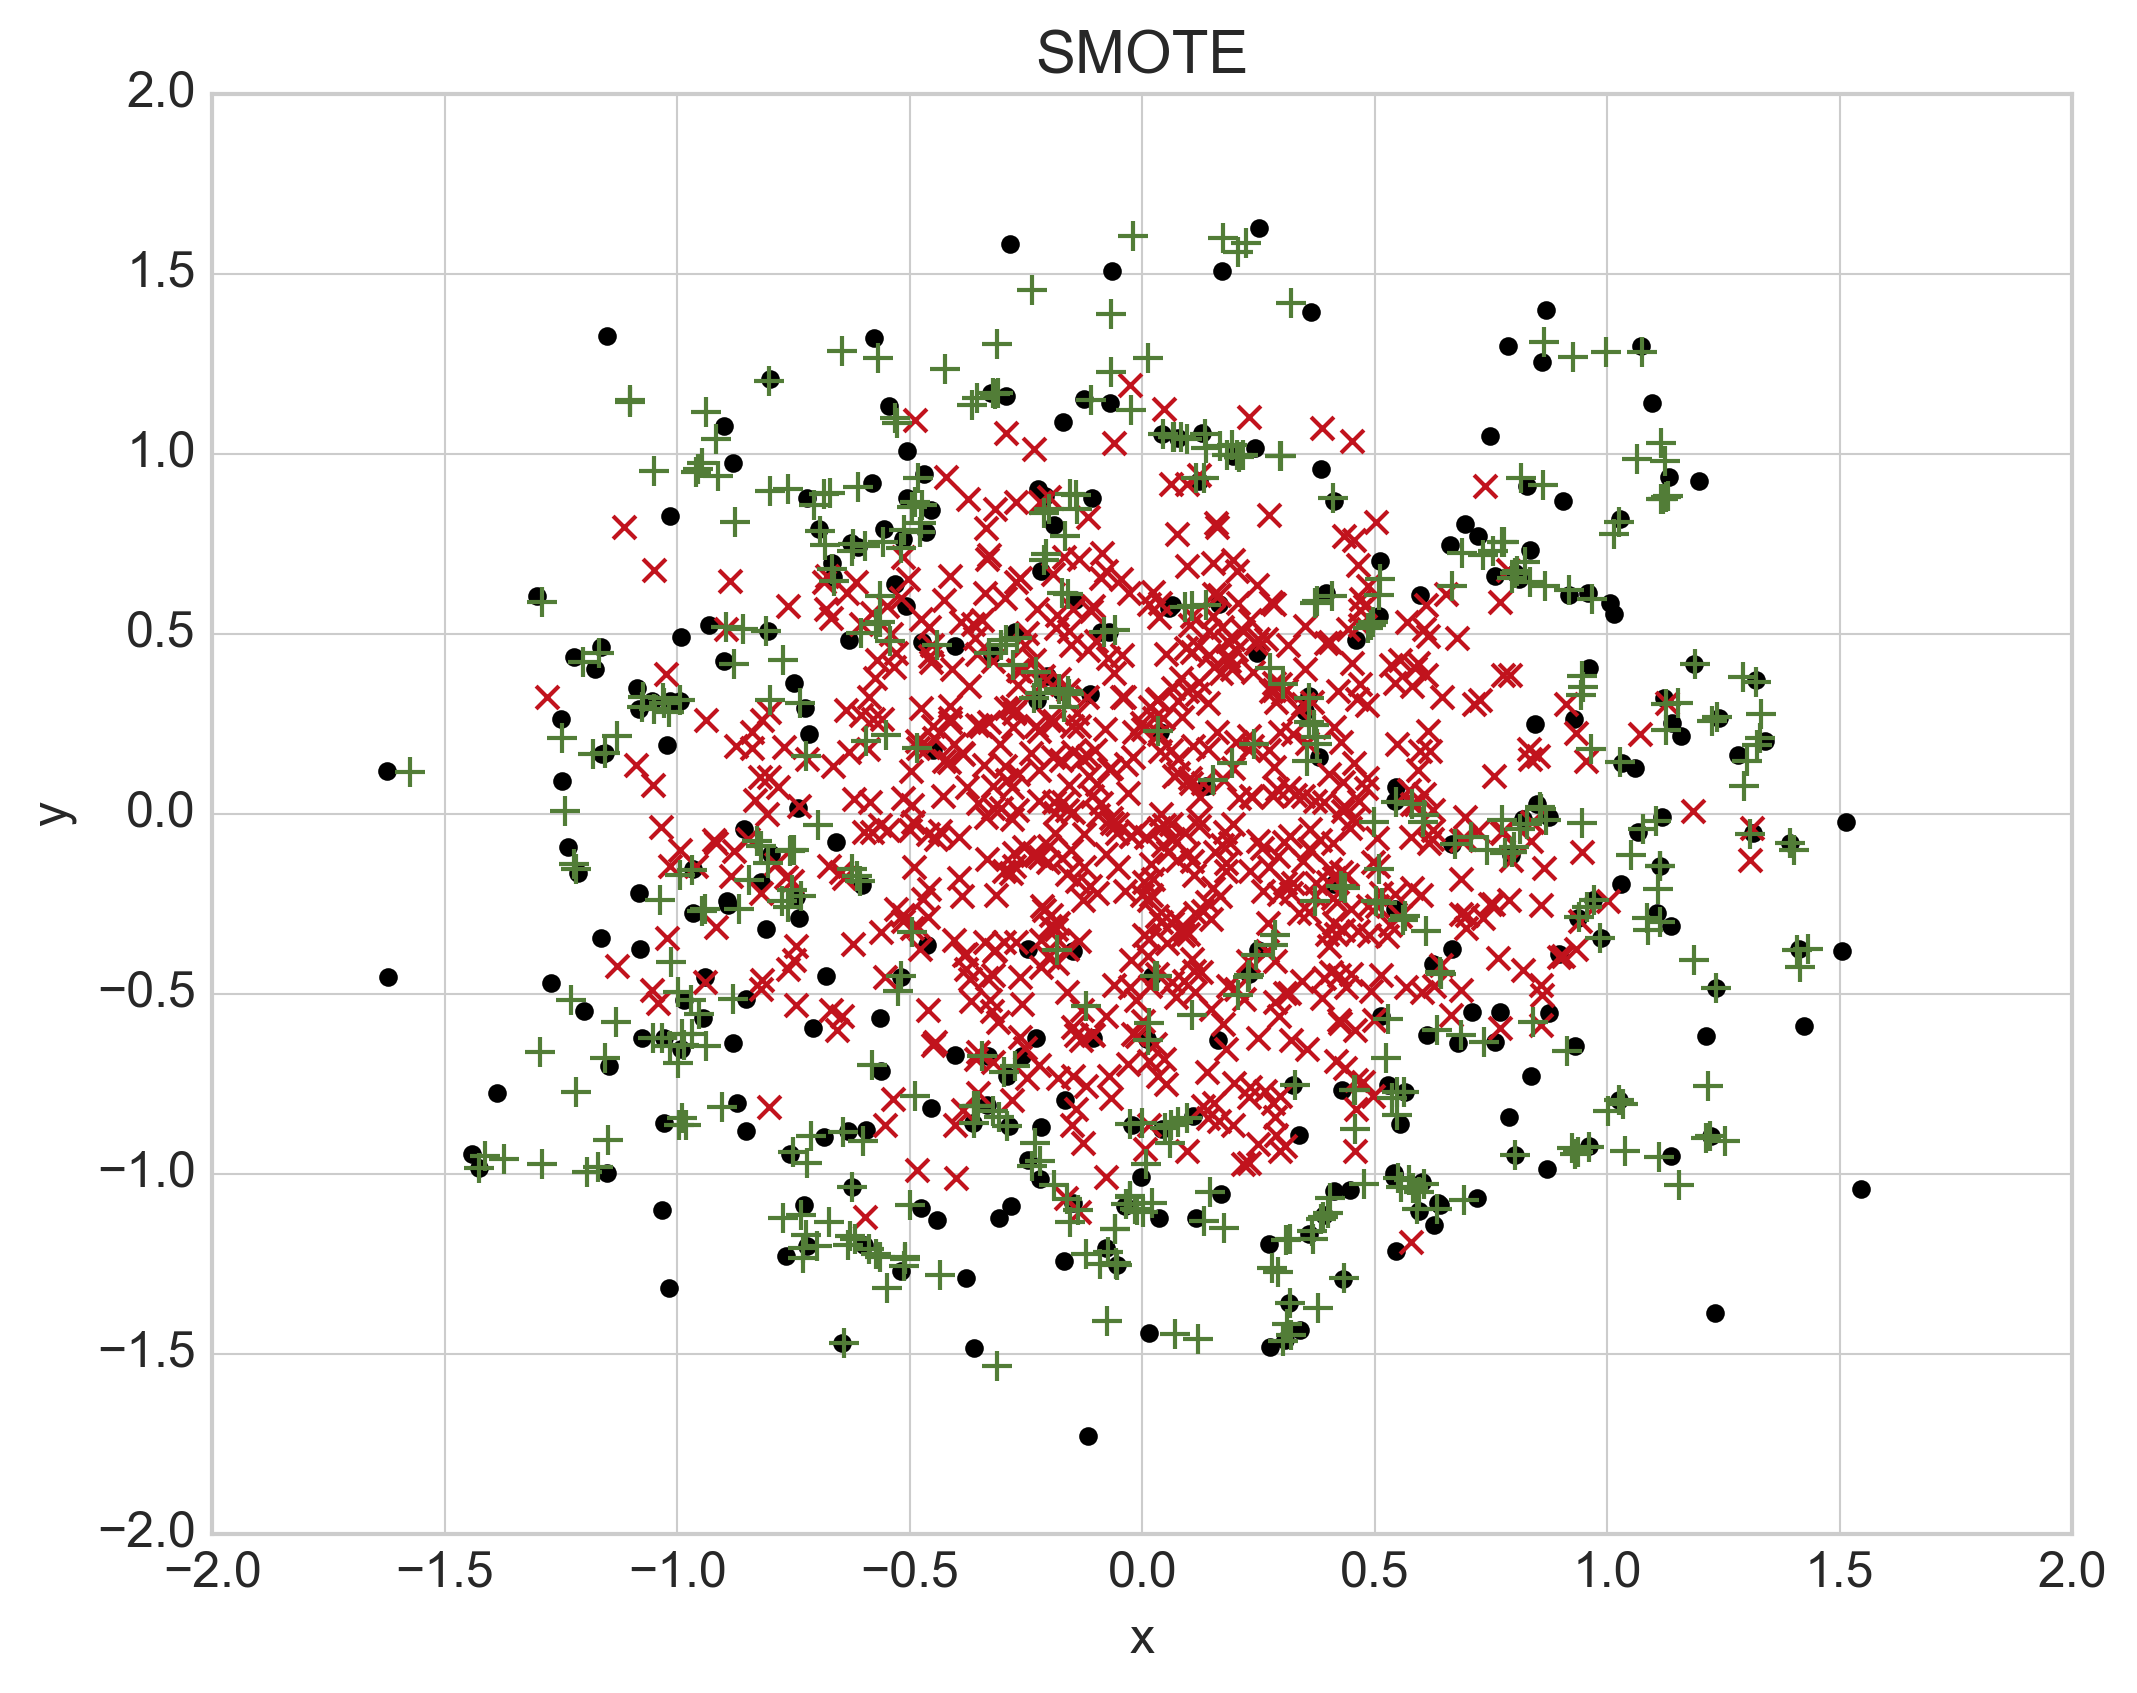
\includegraphics[width=.48\linewidth]{../analysis/Circles_SMOTE.png}
	\hfill
	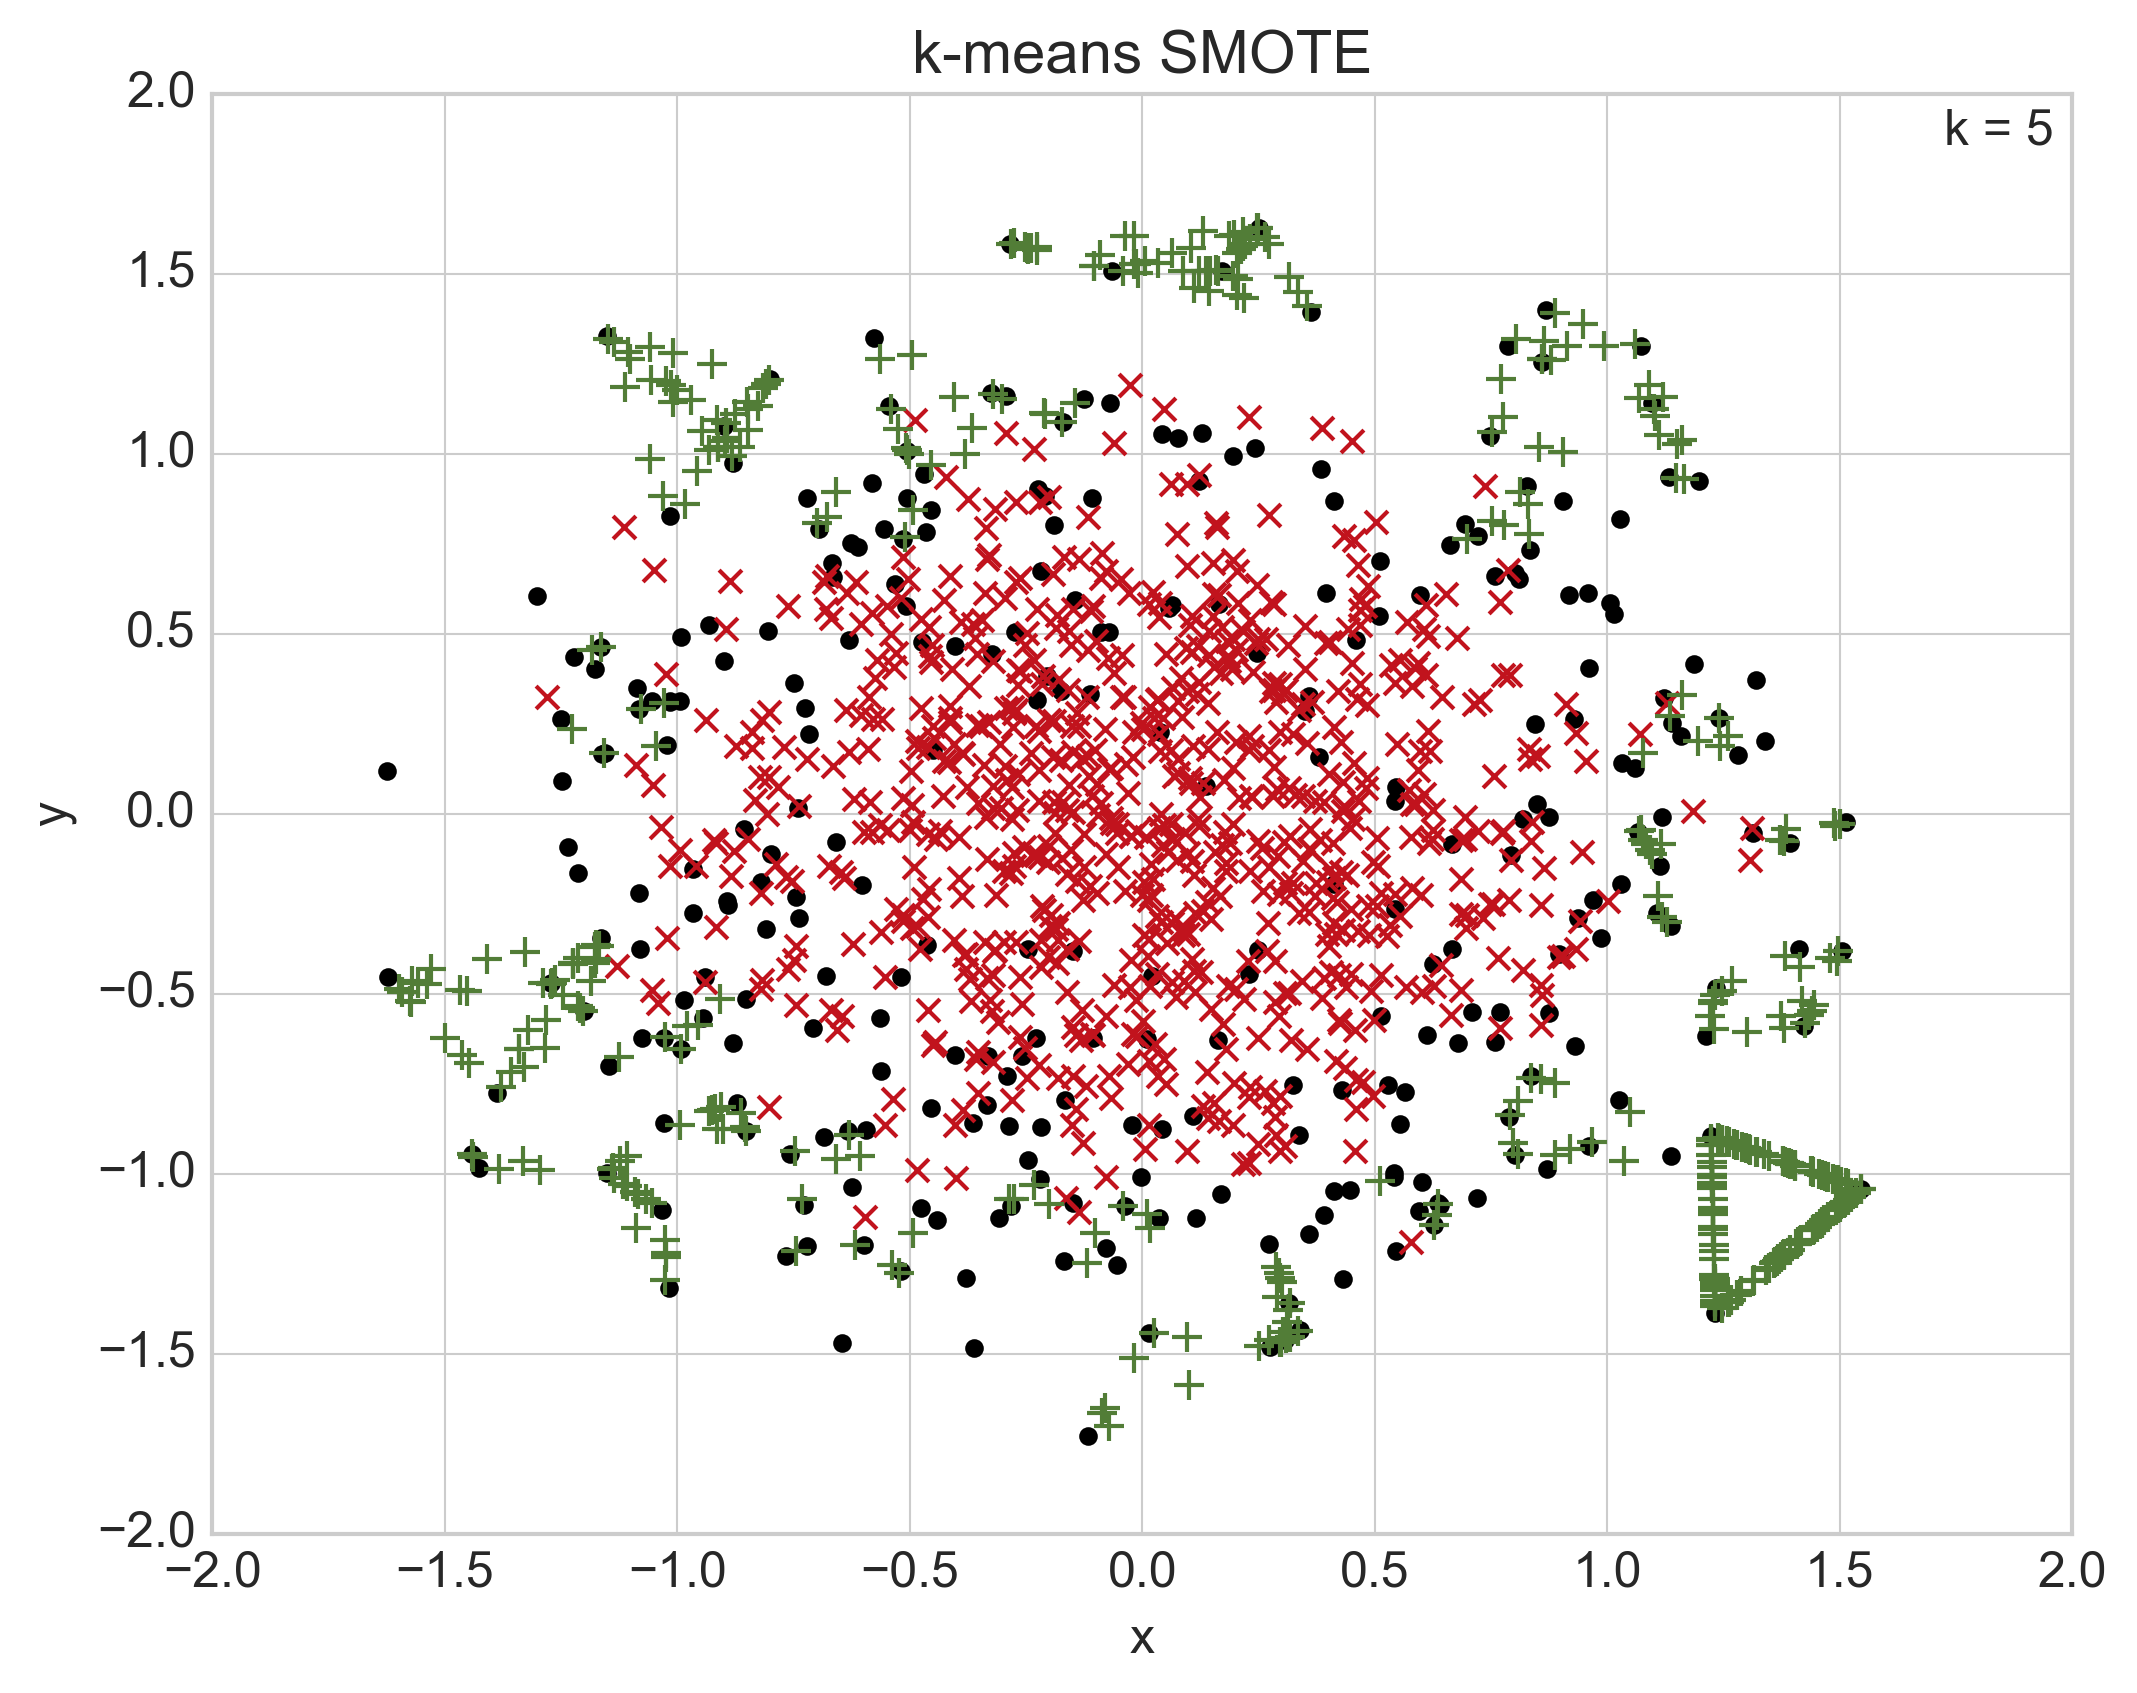
\includegraphics[width=.48\linewidth]{../analysis/Circles_k-means_SMOTE.png}
	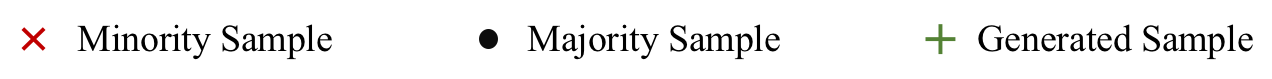
\includegraphics[width=.6\linewidth]{../analysis/legend.png}
	\captionof{figure}{Samples generated through oversampling circles toy dataset with \acs{SMOTE} and k-means \acs{SMOTE}}
	\label{fig:toy-circles}
 \end{figure}

 \begin{figure}[ht]
	\centering
	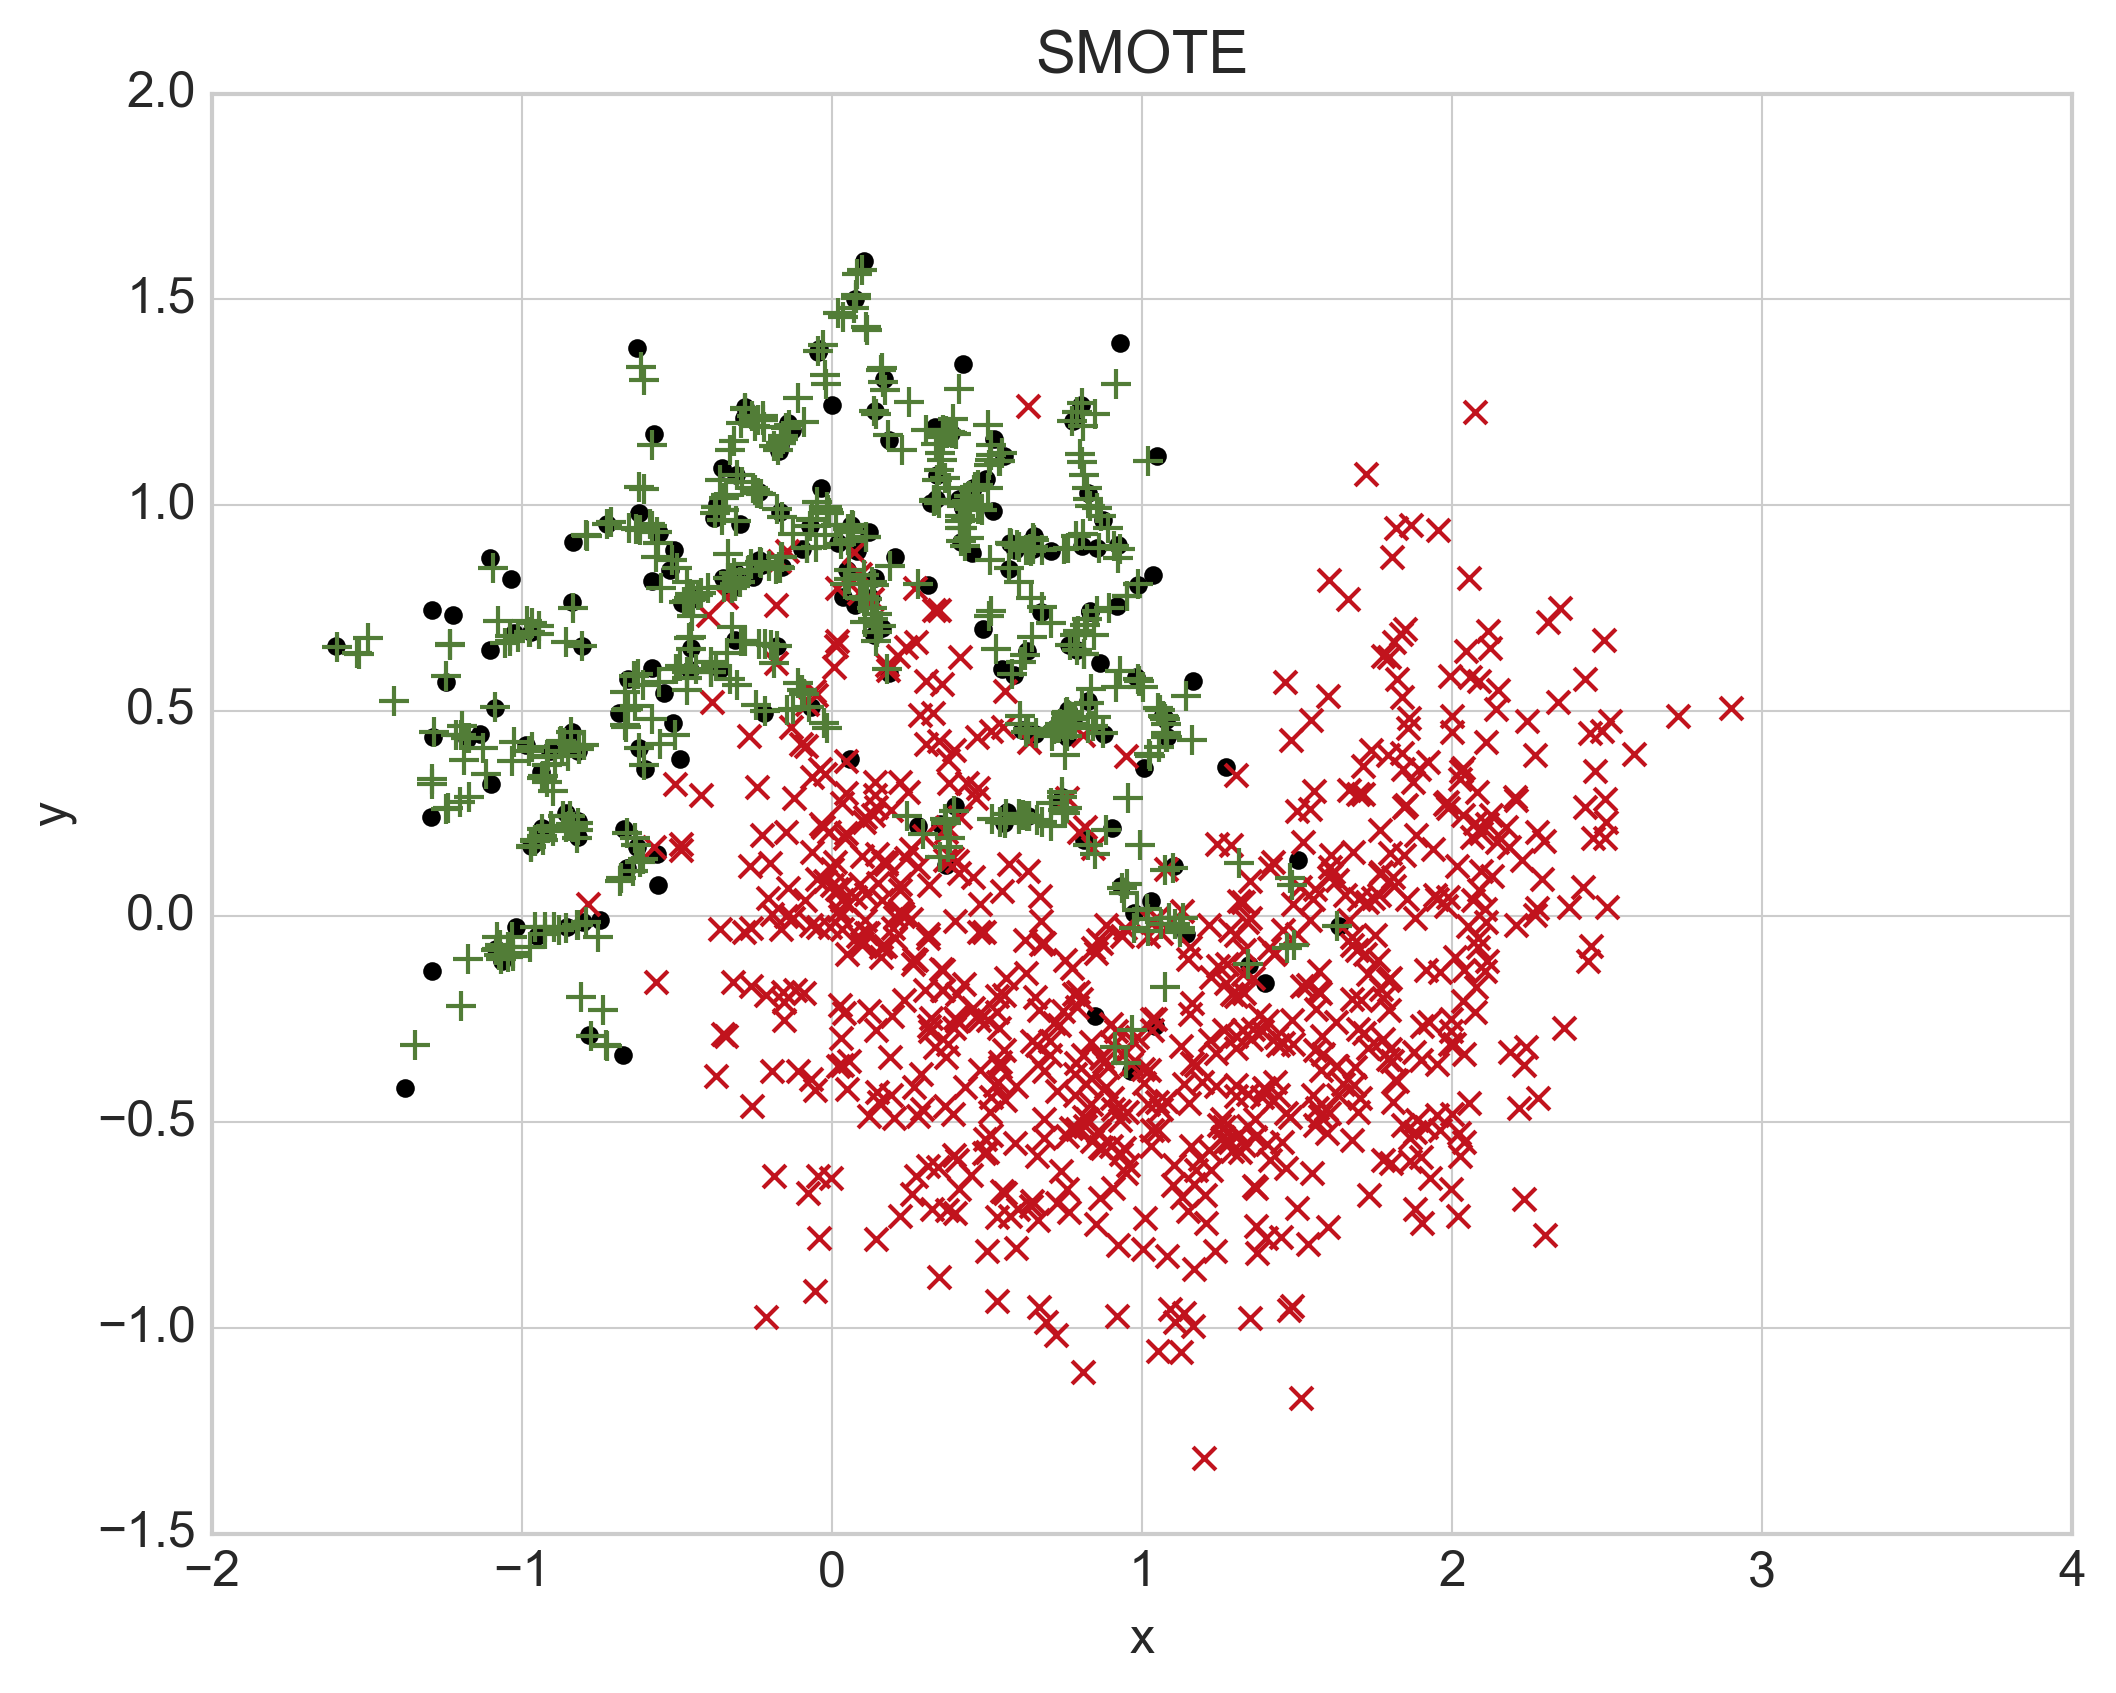
\includegraphics[width=.48\linewidth]{../analysis/Moons_SMOTE.png}
	\hfill
	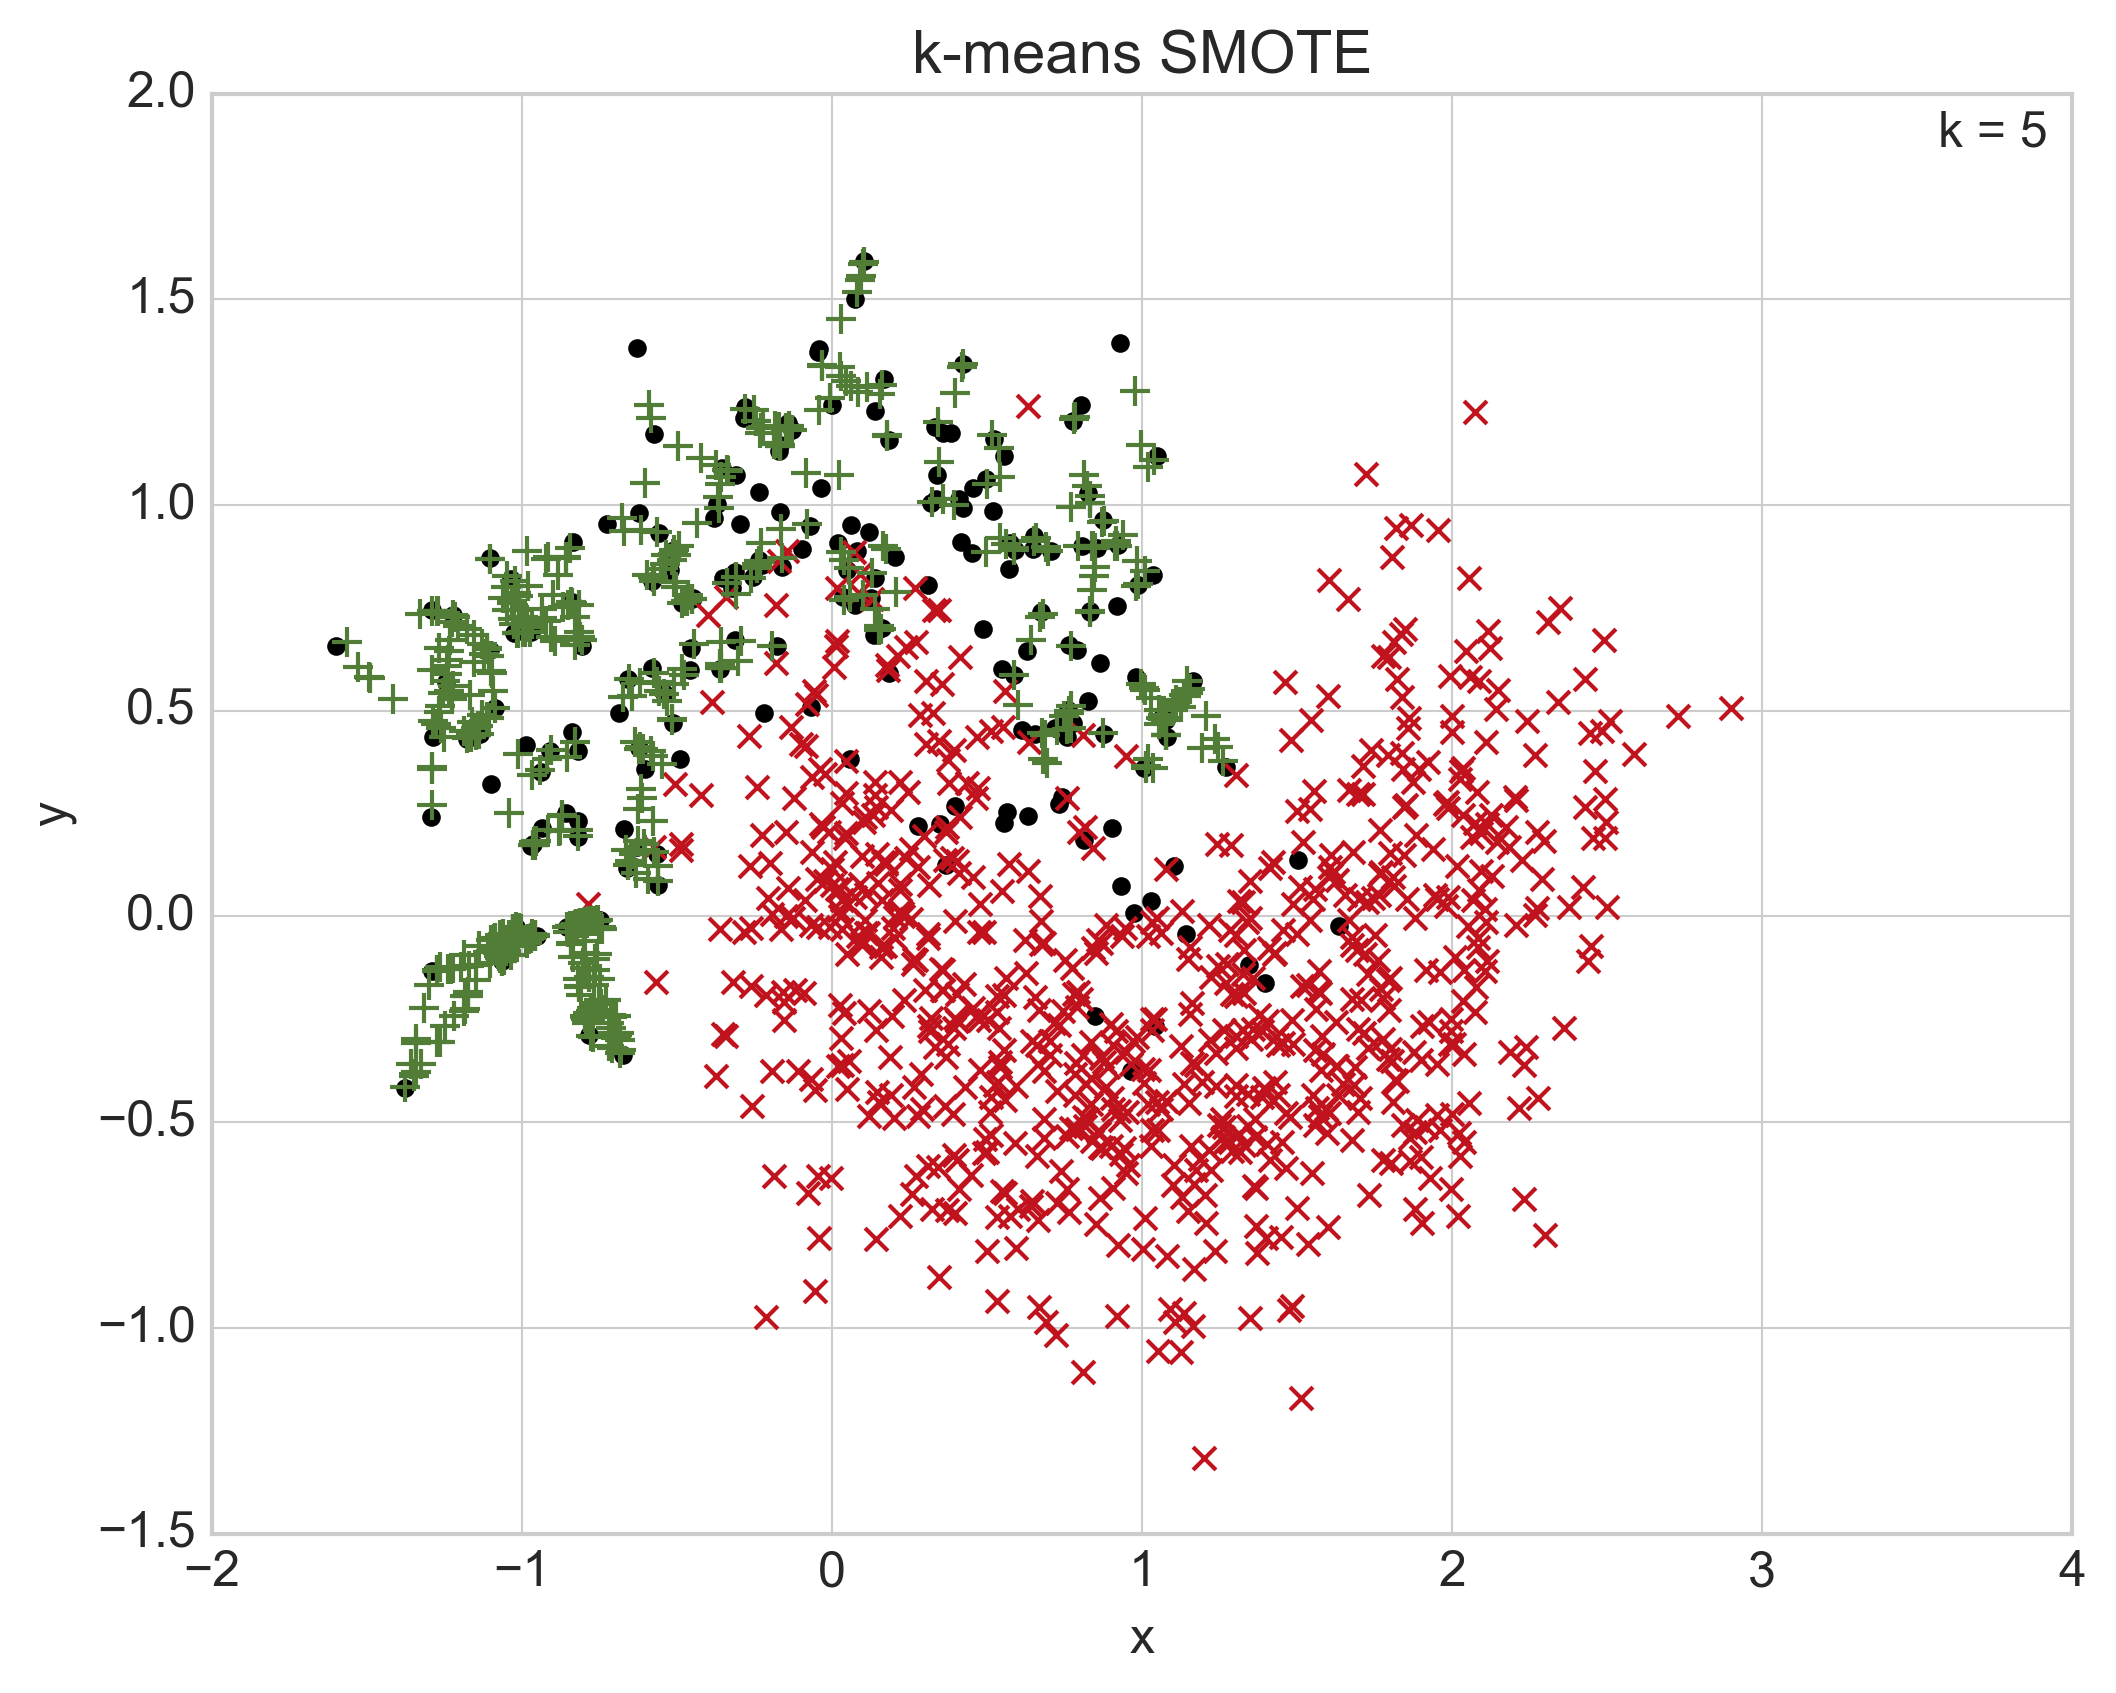
\includegraphics[width=.48\linewidth]{../analysis/Moons_k-means_SMOTE.png}
	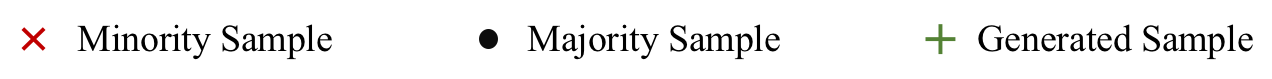
\includegraphics[width=.6\linewidth]{../analysis/legend.png}
	\captionof{figure}{Samples generated through oversampling moons toy dataset with \acs{SMOTE} and k-means \acs{SMOTE}}
	\label{fig:toy-moons}
 \end{figure}

The discussed results are based on 5-fold cross-validation with five
repetitions, using tests to assure statistical significance. Mean ranking
results show that oversampling using k-means \ac{SMOTE} improves the performance
of different evaluated classifiers on imbalanced data. In addition, the proposed
oversampler dominates all evaluated oversampling methods in mean rankings
regardless of the classifier. Studying absolute gains of the proposed algorithm
compared to the baseline method, it is found that all classifiers used in the
study benefit from the clustering and sample distribution procedure of k-means
\ac{SMOTE}. Additionally, results of classifying almost any evaluated dataset
could be improved by applying the proposed method. Generally, classification
problems which are neither very easy nor very difficult profit most, allowing
significant score increases of up to 0.3. Lastly, it is found that the number of
false positives, which are regarded as an indicator of noise generation, can be
effectively reduced by the suggested oversampling technique. Overall it is
concluded that k-means \ac{SMOTE} is effective in generating samples which aid
classifiers in the presence of imbalance.

\section{Conclusion}
\label{sec:conclusion}
Imbalanced data poses a difficult task for many classification algorithms.
Resampling training data toward a more balanced distribution is an effective way
to combat this issue independently of the choice of the classifier. However,
balancing classes by merely duplicating minority class instances encourages
overfitting, which in turn degrades the model's performance on unseen data.
Techniques which generate artificial samples, on the other hand, often suffer
from a tendency to generate noisy samples, impeding the inference of class
boundaries. Moreover, most existing oversamplers do not counteract imbalances
within the minority class, which is often a major issue when classifying
class-imbalanced datasets. For oversampling to effectively aid classifiers, the
amplification of noise should be avoided by detecting safe areas of the input
space where class regions do not overlap. Additionally, any imbalance within the
minority class should be identified and samples are to be generated as to level
the distribution.

The proposed method achieves these properties by clustering the data using
k-means, allowing to focus data generation on crucial areas of the input space.
A high ratio of minority observations is used as an indicator that a cluster is
a safe area. Oversampling only safe clusters enables k-means \ac{SMOTE} to avoid
noise generation. Furthermore, the average distance among a cluster's minority
samples is used to discover sparse areas. Sparse minority clusters are assigned
more synthetic samples, which alleviates within-class imbalance. Finally,
overfitting is discouraged by generating genuinely new observations using
\ac{SMOTE} rather than replicating existing ones.

Empirical results show that training various types of classifiers using data
oversampled with k-means \ac{SMOTE} leads to better classification results than
training with unmodified, imbalanced data. More importantly, the proposed method
consistently outperforms the most widely available oversampling techniques such
as \ac{SMOTE}, borderline-\ac{SMOTE}, and random oversampling. The biggest gains
appear to be achieved in classification problems which are neither extremely
difficult nor extremely simple. Finally, the evaluation of the experiments
conducted shows that the proposed technique effectively reduces noise
generation, which is crucial in many applications. The results are statistically
robust and apply to various metrics suited for the evaluation of imbalanced data
classification.

The effectiveness of the algorithm is accomplished without high complexity. The
method's components, k-means clustering and \ac{SMOTE} oversampling, are simple
and readily available in many programming languages, so that practitioners and
researchers may easily implement and use the proposed method in their preferred
environment. Further facilitating practical use, an implementation of k-means
\ac{SMOTE} in the Python programming language is made available (see
\url{https://github.com/felix-last/kmeans_smote}) based on the imbalanced-learn
framework \citep{Lemaitre.2017}.

A prevalent issue in classification tasks, data imbalance is exhibited naturally
in many important real-world applications. As the proposed oversampler can be
applied to rebalance any dataset and independently of the chosen classifier, its
potential impact is substantial. Among others, k-means \ac{SMOTE} may,
therefore, contribute to the prevention of credit card fraud, the diagnosis of
diseases, as well as the detection of abnormalities in environmental
observations.

Future work may consequently focus on applying k-means \ac{SMOTE} to various
other real-world problems. Additionally, finding optimal values of $k$ and other
hyperparameters is yet to be guided by rules of thumb, which could be deducted
from further analyses of the relationship between optimal hyperparameters for a
given dataset and the dataset's properties.

\bibliographystyle{./elsarticle-num-names-alphsort.bst}
\bibliography{references}

\end{document}
